% !TeX program = lualatex
% !TeX encoding = utf8

\documentclass[aspectratio=169, 10pt]{beamer}

\usepackage{amsmath}
\usepackage[T1]{fontenc}

\usepackage{lhcb_presentation/package}

\usepackage{units}
\usepackage{graphicx}
\usepackage{booktabs}
\usepackage{ulem}
\usepackage{bm}
\usepackage{comment}
\usepackage{tikz}
\definecolor{brickred}{rgb}{0.85, 0, 0.05}
\errorcontextlines 10000

\title[PV finding with CNNs: LHCb Computing Workshop 2018]{PV finding with CNNs\\{\small LHCb Computing Workshop 2018}}

\author[Fang, Schreiner, Sokoloff]{Rui Fang \and Henry Schreiner \and Mike Sokoloff}
\institute{The University of Cincinnati}
\date{September 26, 2018}


\begin{document}

\begin{frame}
\titlepage
\end{frame}

\section{Introduction}
% Part 1: HENRY
\subsection{Objectives}
\begin{frame}{Objectives}
\begin{columns}[c]
    \column{.5\textwidth}
    \begin{block}{Physics}
    \begin{itemize}
        \item Iterative tracking and vertexing may allow high efficiency, high speed, highly parallel algorithms:
        \begin{itemize}
            \item {\bf Use proto-tracks to find primary vertex (PV) candidates}
            \item Use PV candidates to augment more complete tracking
            \item Find more PVs plus secondary vertices
        \end{itemize}
        \item PVs available quickly
    \end{itemize}
    \end{block}
    \column{.5\textwidth}
    \begin{block}{Machine learning}
    \begin{itemize}
        \item Sparse 3D data (41M pixels) $\to$ rich 1D dataset
        \item 1D convolutional neural net
        \item Great opportunities to visualize learning process
    \end{itemize}
    \end{block}

    \begin{block}{Computation}
    \begin{itemize}
        \item Highly parallelizable
        \item Well suited to GPUs
    \end{itemize}
    \end{block}
\end{columns}


\end{frame}

\subsection{Tracking in the LHCb upgrade}
\begin{frame}{Tracking in the LHCb upgrade}
  \begin{columns}[c]
    \column{.5\textwidth}
    \begin{block}{The changes}
      \begin{itemize}
          \item 30 MHz software trigger
          \item 7.6 PVs per event (Poisson distribution)
      \end{itemize}
    \end{block}
    \begin{block}{The problem}
    \begin{itemize}
    	\item Much higher pileup
    	\item Very little time to do the tracking
    	\item Current algorithms too slow
    \end{itemize}
    \end{block}
    \column{.5\textwidth}
      \begin{center}
    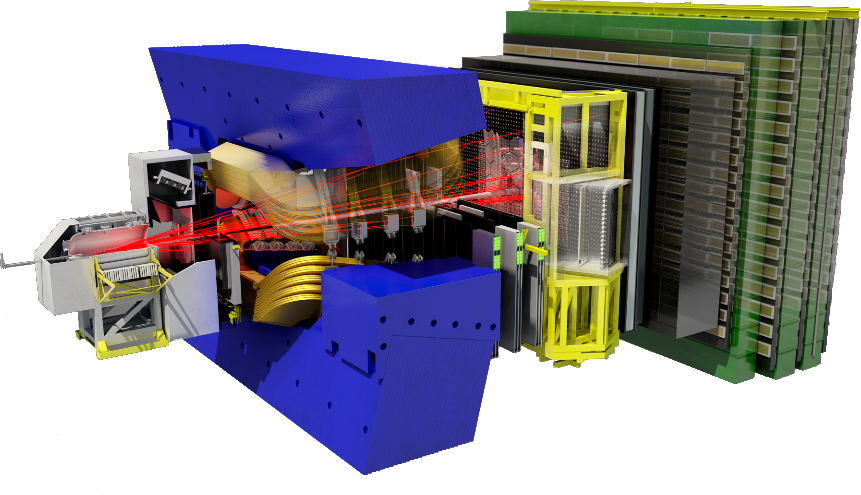
\includegraphics[width=\textwidth, trim=18 0 18 0]{images/LHCbDet.png}
  \end{center}
  \end{columns}

  \vspace{1em}
  \begin{center}
    \textbf{We need to rethink our algorithms from the ground up...}
  \end{center}
\end{frame}

\subsection{A hybrid ML approach}
\begin{frame}{A hybrid ML approach}
\begin{center}
Prototracking $\rightarrow$ Kernel generation $\rightarrow$ CNN to find PVs $\rightarrow$ Informed tracking
\end{center}

\begin{columns}[b]
    \column{.28\textwidth}
    \begin{block}{Prototracking}
    \begin{itemize}
        \item Ultra-simple/fast
        \item Triplets only
        \item Used for kernel only
        \end{itemize}
    \end{block}
    \column{.30\textwidth}
    \begin{block}{Vertexing}
    \begin{itemize}
        \item High efficiency
        \item Low false positive rate
        \item Useful for other reasons
        \end{itemize}
    \end{block}
    \column{.28\textwidth}
    \begin{block}{Tracking}
    \begin{itemize}
        \item Faster (effect TBD)
        \item Uses search windows
        \item Higher efficiency
    \end{itemize}
    \end{block}
\end{columns}
    \begin{block}{Machine learning features (so far)}
        \begin{itemize}
            \item Prototracking converts sparse 3D dataset to feature-rich 1D dataset
            \item Easy and effective visualization due to 1D nature
            \item Can see results with simple unoptimized 2-layer CNN + 1-layer linear
        \end{itemize}
    \end{block}

\vspace{.3em}
\begin{center}
What follows is a proof of principle implementation for finding PVs.
\end{center}
\end{frame}

\subsection{Vertices and tracks}
\begin{frame}{Vertices and tracks}
\begin{columns}[c]
    \column{.5\textwidth}
    \begin{block}{Vertices}
      \begin{itemize}
          \item Events contain $\approx 7$ Primary Vertices (PVs)
          \begin{itemize}
            \item A PV should contain 5+ long tracks
          \end{itemize}
          \item Multiple Secondary Vertices (SVs) per event as well
          \begin{itemize}
            \item A SV should contain 2+ tracks
          \end{itemize}
      \end{itemize}
    \end{block}

    \column{.5\textwidth}
    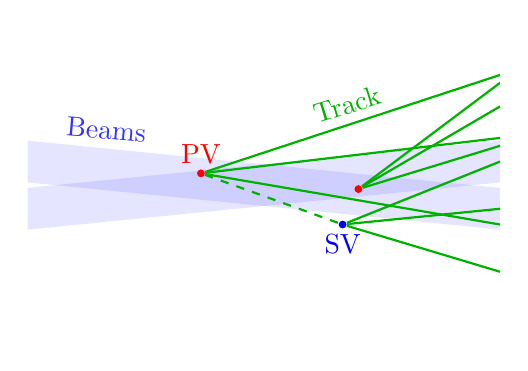
\begin{tikzpicture}
        [beam/.style={line width = 15, opacity=.1, blue, shorten >= -.2cm, shorten <= -.2cm},
        PV/.style={red, circle, fill, inner sep=1pt},
        SV/.style={blue, circle, fill, inner sep=1pt},
        track/.style={green!70!black, thick}]

        \clip [use as bounding box] (-3,-2) rectangle (3,2);
        \clip (-3,-2) rectangle (3,2);

        \node [blue!80!white, rotate=-5] at (-2, .7) {Beams};
        \draw [beam] (-3,.3) -- (3,-.3);
        \draw [beam] (-3,-.3) -- (3,.3);

        \node [PV] (A) at (1.2, -.05) {};
        \node [PV] (B) at (-.8, .15) {};
        \node [red, above] at (B) {PV};

        \draw [track] (A) -- (3,1.3);
        \draw [track] (A) -- (3,1);
        \draw [track] (A) -- (3,.5);

        \draw [track] (B) -- (3,1.4) node [midway, above, rotate=17] {Track};
        \draw [track] (B) -- (3,.6);
        \draw [track] (B) -- (3,-.5);
        \draw [track, dashed] (B) -- (1,-.5);

        \node [SV] (C) at (1,-.5) {};
        \node [blue, below] at (C) {SV};
        \draw [track] (C) -- (3, -.3);
        \draw [track] (C) -- (3, .3);
        \draw [track] (C) -- (3, -1.1);
    \end{tikzpicture}
  \end{columns}

  \begin{block}{}
  \begin{itemize}
      \item We are developing a way to find PVs and SVs using hit triplets
      \item This will enable an iterative tracking algorithm
  \end{itemize}
  \end{block}
\end{frame}


\section{Design}

\subsection{Kernel Generation}
\begin{frame}{Kernel Generation}
  \begin{columns}[c]
    \column{.54\textwidth}
    \only<1>{%
        \begin{block}{Hits}
        \begin{itemize}
            \item Hits lie on the 26 planes
            \item Tracks come from PVs and SVs
            \item For simplicity, only 3 tracks shown
            \item Hits are sorted in $r$ (distance from LHC beam)
        \end{itemize}
        \end{block}
    }
    \only<2>{%
        \begin{block}{Grid}
        \begin{itemize}
            \item Make a 3D grid of voxels (2D shown)
            \item \textcolor{brickred}{Note: only $z$ will be fully calculated and stored}
        \end{itemize}
        \end{block}
    }
    \only<3-5>{%
        \begin{block}{Prototrack}
        \begin{itemize}
            \item Start with maximum $r$
            \item Find triplet with $\chi^2<10$
            \item Mark ``used'' all other hits within $\chi^2<9$
            \item \textcolor{brickred}{Note: triplet is stored}
        \end{itemize}
        \end{block}
        
        \begin{block}{Kernel}
        \begin{itemize}
            \item Fill in each voxel center with gaussian PDF
            \item PDF is combined for each prototrack
        \end{itemize}
        \end{block}
        
    }
    \only<6>{%
        \begin{block}{Kernel}
        \begin{itemize}
            \item Highest PDF density at vertices
            \item Stores $z$ histogram with maximum PDF values
        \end{itemize}
        \end{block}
        
        \begin{block}{Details}
        \begin{itemize} \color{brickred}
            \item $x$-$y$ grid initially very coarse
            \item Search performed on maximum $x$-$y$ grid cell using stored triplets to recalculate PDF
        \end{itemize}
        \end{block}
    }
    
    \column{.46\textwidth}
    \begin{tikzpicture}
        [hit/.style={inner sep=2pt, fill, circle, black!80!red},
        simitrack/.style={shorten >= -6cm, shorten <= -6cm, opacity=.2, line width=.1cm,
            preaction={draw, line width=.3cm, opacity=.2},
            preaction={draw, line width=.5cm, opacity=.2}},
        bluesimitrack/.style={thick, blue,
            preaction={shorten >= -6cm, shorten <= -6cm, draw, opacity=.2, line width=.1cm,
                preaction={draw, blue, line width=.3cm, opacity=.2},
                preaction={draw, blue, line width=.5cm, opacity=.2}}}
        ]
        
        \node at (2,-3) [below] {$z$ axis (along the beam)};
        \node at (-1, 0) [left] {$x$};
        
        \clip (-1,-3) rectangle (5,3);
        
        \begin{scope}[xscale=.65, xshift=-.6cm]
        
        % def f(name, slope, factor):
        %     v = np.arange(1,9)
        %     vv = (v-.5)*slope + .05*np.sin(v*factor)
        %     q = np.linspace(.5, 8, 400)
        %     qq = (q-.5)*slope + .05*np.sin(q*factor)
        %     print(f'% {name} slope={slope} factor={factor}')
        %     for a,b in zip(v,vv):
        %         print(f'\coordinate ({name}{a}) at ({a}, {b:.3});')
        %     print()
        %     return q, qq, v, vv

        
        % (v-.5)*slope + .05*np.sin(v*factor)
        % A slope=0.4 factor=-5
        \coordinate (A1) at (1, 0.248);
        \coordinate (A2) at (2, 0.627);
        \coordinate (A3) at (3, 0.967);
        \coordinate (A4) at (4, 1.35);
        \coordinate (A5) at (5, 1.81);
        \coordinate (A6) at (6, 2.25);
        \coordinate (A7) at (7, 2.62);
        
        % B slope=0.06 factor=6
        \coordinate (B1) at (1, 0.016);
        \coordinate (B2) at (2, 0.0632);
        \coordinate (B3) at (3, 0.112);
        \coordinate (B4) at (4, 0.165);
        \coordinate (B5) at (5, 0.221);
        \coordinate (B6) at (6, 0.28);
        \coordinate (B7) at (7, 0.344);
        \coordinate (B8) at (8, 0.412);
        
        % C slope=-0.35 factor=7
        \coordinate (C1) at (1, -0.142);
        \coordinate (C2) at (2, -0.475);
        \coordinate (C3) at (3, -0.833);
        \coordinate (C4) at (4, -1.21);
        \coordinate (C5) at (5, -1.6);
        \coordinate (C6) at (6, -1.97);
        \coordinate (C7) at (7, -2.32);
        
        \only<1>{%
        \foreach \x in {0,...,9}{%
            \draw [ultra thick, yellow!80!black] (\x, -3) -- (\x,3);
        }
        }
        \end{scope}
        
        \only<2->{%
        \draw[step=.5, gray, very thin, use as bounding box] (-1,-3) grid (5,3);
        }
        
        \only<3>{%
            \draw [bluesimitrack] (A5) -- (A7) ;
        } \only<4->{%
            \draw [simitrack] (A5) -- (A7) ;
        }
        
        \only<4>{%
            \draw [bluesimitrack] (B6) -- (B8) ;
        } \only<5->{%
            \draw [simitrack] (B6) -- (B8) ;
        }
        
        \only<5>{%
            \draw [bluesimitrack] (C5) -- (C7) ;
        } \only<6->{%
            \draw [simitrack] (C5) -- (C7) ;
        }
        
        \draw [fill,green!60!black] (0,0) circle (.065) node [left] {PV};
        
        \only<0-2>{%
        \node [hit] at (A1) {};
        \node [hit] at (A2) {};
        \node [hit] at (A3) {};
        \node [hit] at (A4) {};
        }\only<3->{%
        \node [hit, red] at (A1) {};
        \node [hit, red] at (A2) {};
        \node [hit, red] at (A3) {};
        \node [hit, red] at (A4) {};
        }
        
        \only<0-2>{%
        \node [hit] at (A5) {};
        \node [hit] at (A6) {};
        \node [hit] at (A7) {};
        } \only<3>{%
        \node [hit, blue] at (A5) {};
        \node [hit, blue] at (A6) {};
        \node [hit, blue] at (A7) {};
        } \only<4->{%
        \node [hit, red] at (A5) {};
        \node [hit, red] at (A6) {};
        \node [hit, red] at (A7) {};
        }
        
        \only<0-3>{%
        \node [hit] at (B1) {};
        \node [hit] at (B2) {};
        \node [hit] at (B3) {};
        \node [hit] at (B4) {};
        \node [hit] at (B5) {};
        \node [hit] at (C1) {};
        } \only<4->{%
        \node [hit, red] at (B1) {};
        \node [hit, red] at (B2) {};
        \node [hit, red] at (B3) {};
        \node [hit, red] at (B4) {};
        \node [hit, red] at (B5) {};
        \node [hit, red] at (C1) {};
        }
        
        \only<0-3>{%
        \node [hit] at (B6) {};
        \node [hit] at (B7) {};
        \node [hit] at (B8) {};
        } \only<4>{%
        \node [hit, blue] at (B6) {};
        \node [hit, blue] at (B7) {};
        \node [hit, blue] at (B8) {};
        }\only<5->{%
        \node [hit, red] at (B6) {};
        \node [hit, red] at (B7) {};
        \node [hit, red] at (B8) {};
        }
        
        \only<0-4>{%
        \node [hit] at (C2) {};
        \node [hit] at (C3) {};
        \node [hit] at (C4) {};
        } \only<5->{%
        \node [hit, red] at (C2) {};
        \node [hit, red] at (C3) {};
        \node [hit, red] at (C4) {};
        }
        
        \only<0-4>{%
        \node [hit] at (C5) {};
        \node [hit] at (C6) {};
        \node [hit] at (C7) {};
        } \only<5>{%
        \node [hit, blue] at (C5) {};
        \node [hit, blue] at (C6) {};
        \node [hit, blue] at (C7) {};
        } \only<6->{%
        \node [hit, red] at (C5) {};
        \node [hit, red] at (C6) {};
        \node [hit, red] at (C7) {};
        }
        
    \end{tikzpicture}

    \end{columns}
\end{frame}


% Part 3: HENRY
\subsection{Example of z KDE histogram}
\begin{frame}{Example of z KDE histogram}
\begin{center}
    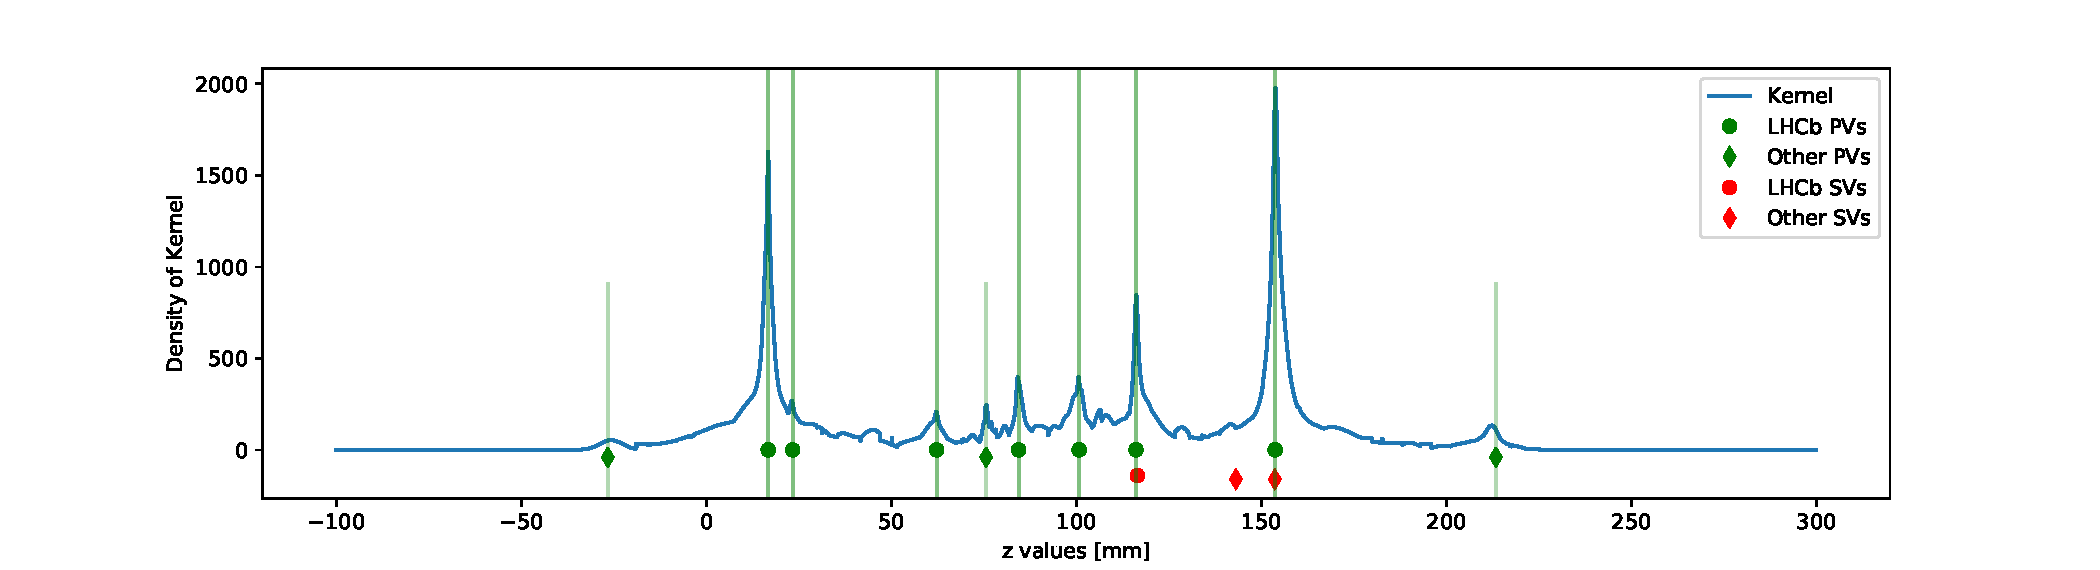
\includegraphics[width=\textwidth, trim=50 30 50 30]{images/kernel_and_pvs.pdf}
\end{center}
\begin{columns}[t]
    \column{.55\textwidth}
    \begin{block}{Human learning}
    \begin{itemize}
        \item Peaks generally correspond to PVs and SVs
    \end{itemize}
    \end{block}
    
    \column{.45\textwidth}
    \begin{block}{Challenges}
    \begin{itemize}
        \item Vertex may be offset from peak
        \item Vertices interact
    \end{itemize}
    \end{block}
\end{columns}
\end{frame}

% Zoom in

% rui add a target histogram
\subsection{Distribution of Target}
\begin{frame}{Target distribution}
\begin{columns}[c]
    \column{.5\textwidth}
    \begin{block}{Build target distribution}
      \begin{itemize}
          \item real PV position as the mean of Gaussian distribution 
          \item $\sigma $(standard deviation) is 100 $\mu$m
          \item calculate the cdf of each bin around of the mean, within $\pm$ 3 bins ($\pm$ 300 $\mu$m )
      \end{itemize}
    \end{block}
    \begin{center}
            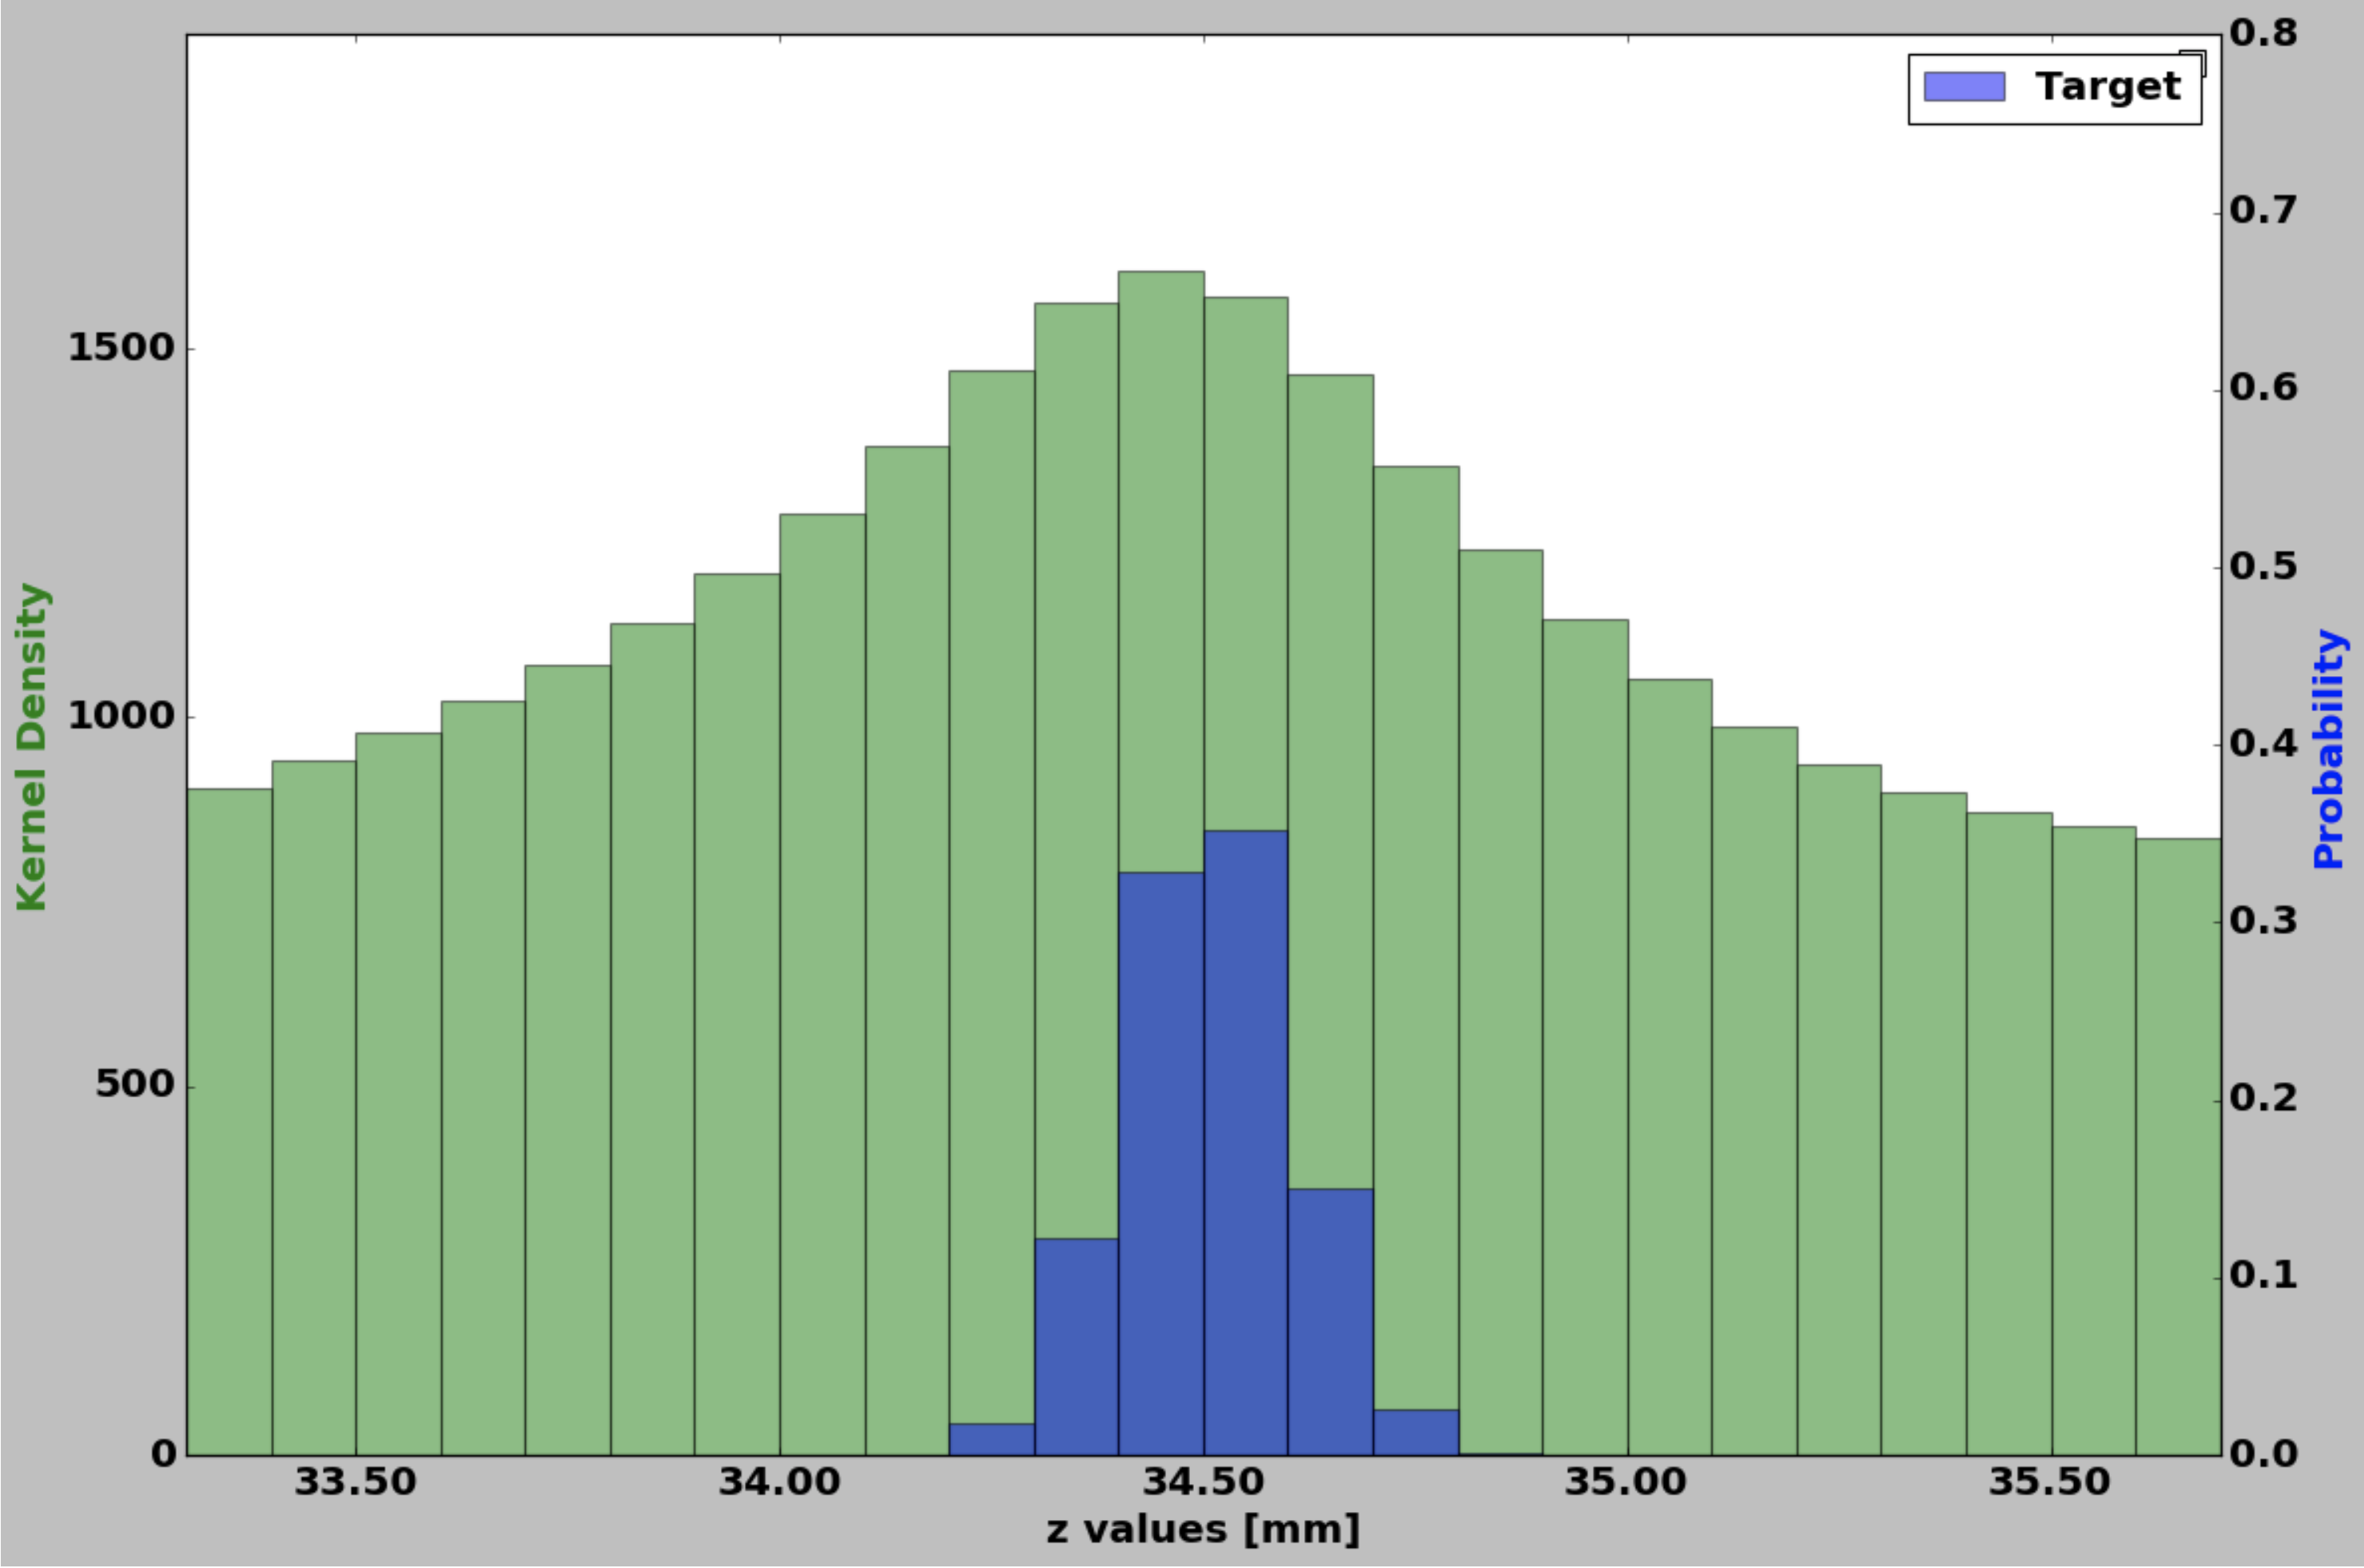
\includegraphics[width=1\textwidth,height=0.45\textwidth,trim=18 0 18 0]{images/T_1_12.png}
            
        \end{center}
    \column{.5\textwidth}
      \begin{center}
    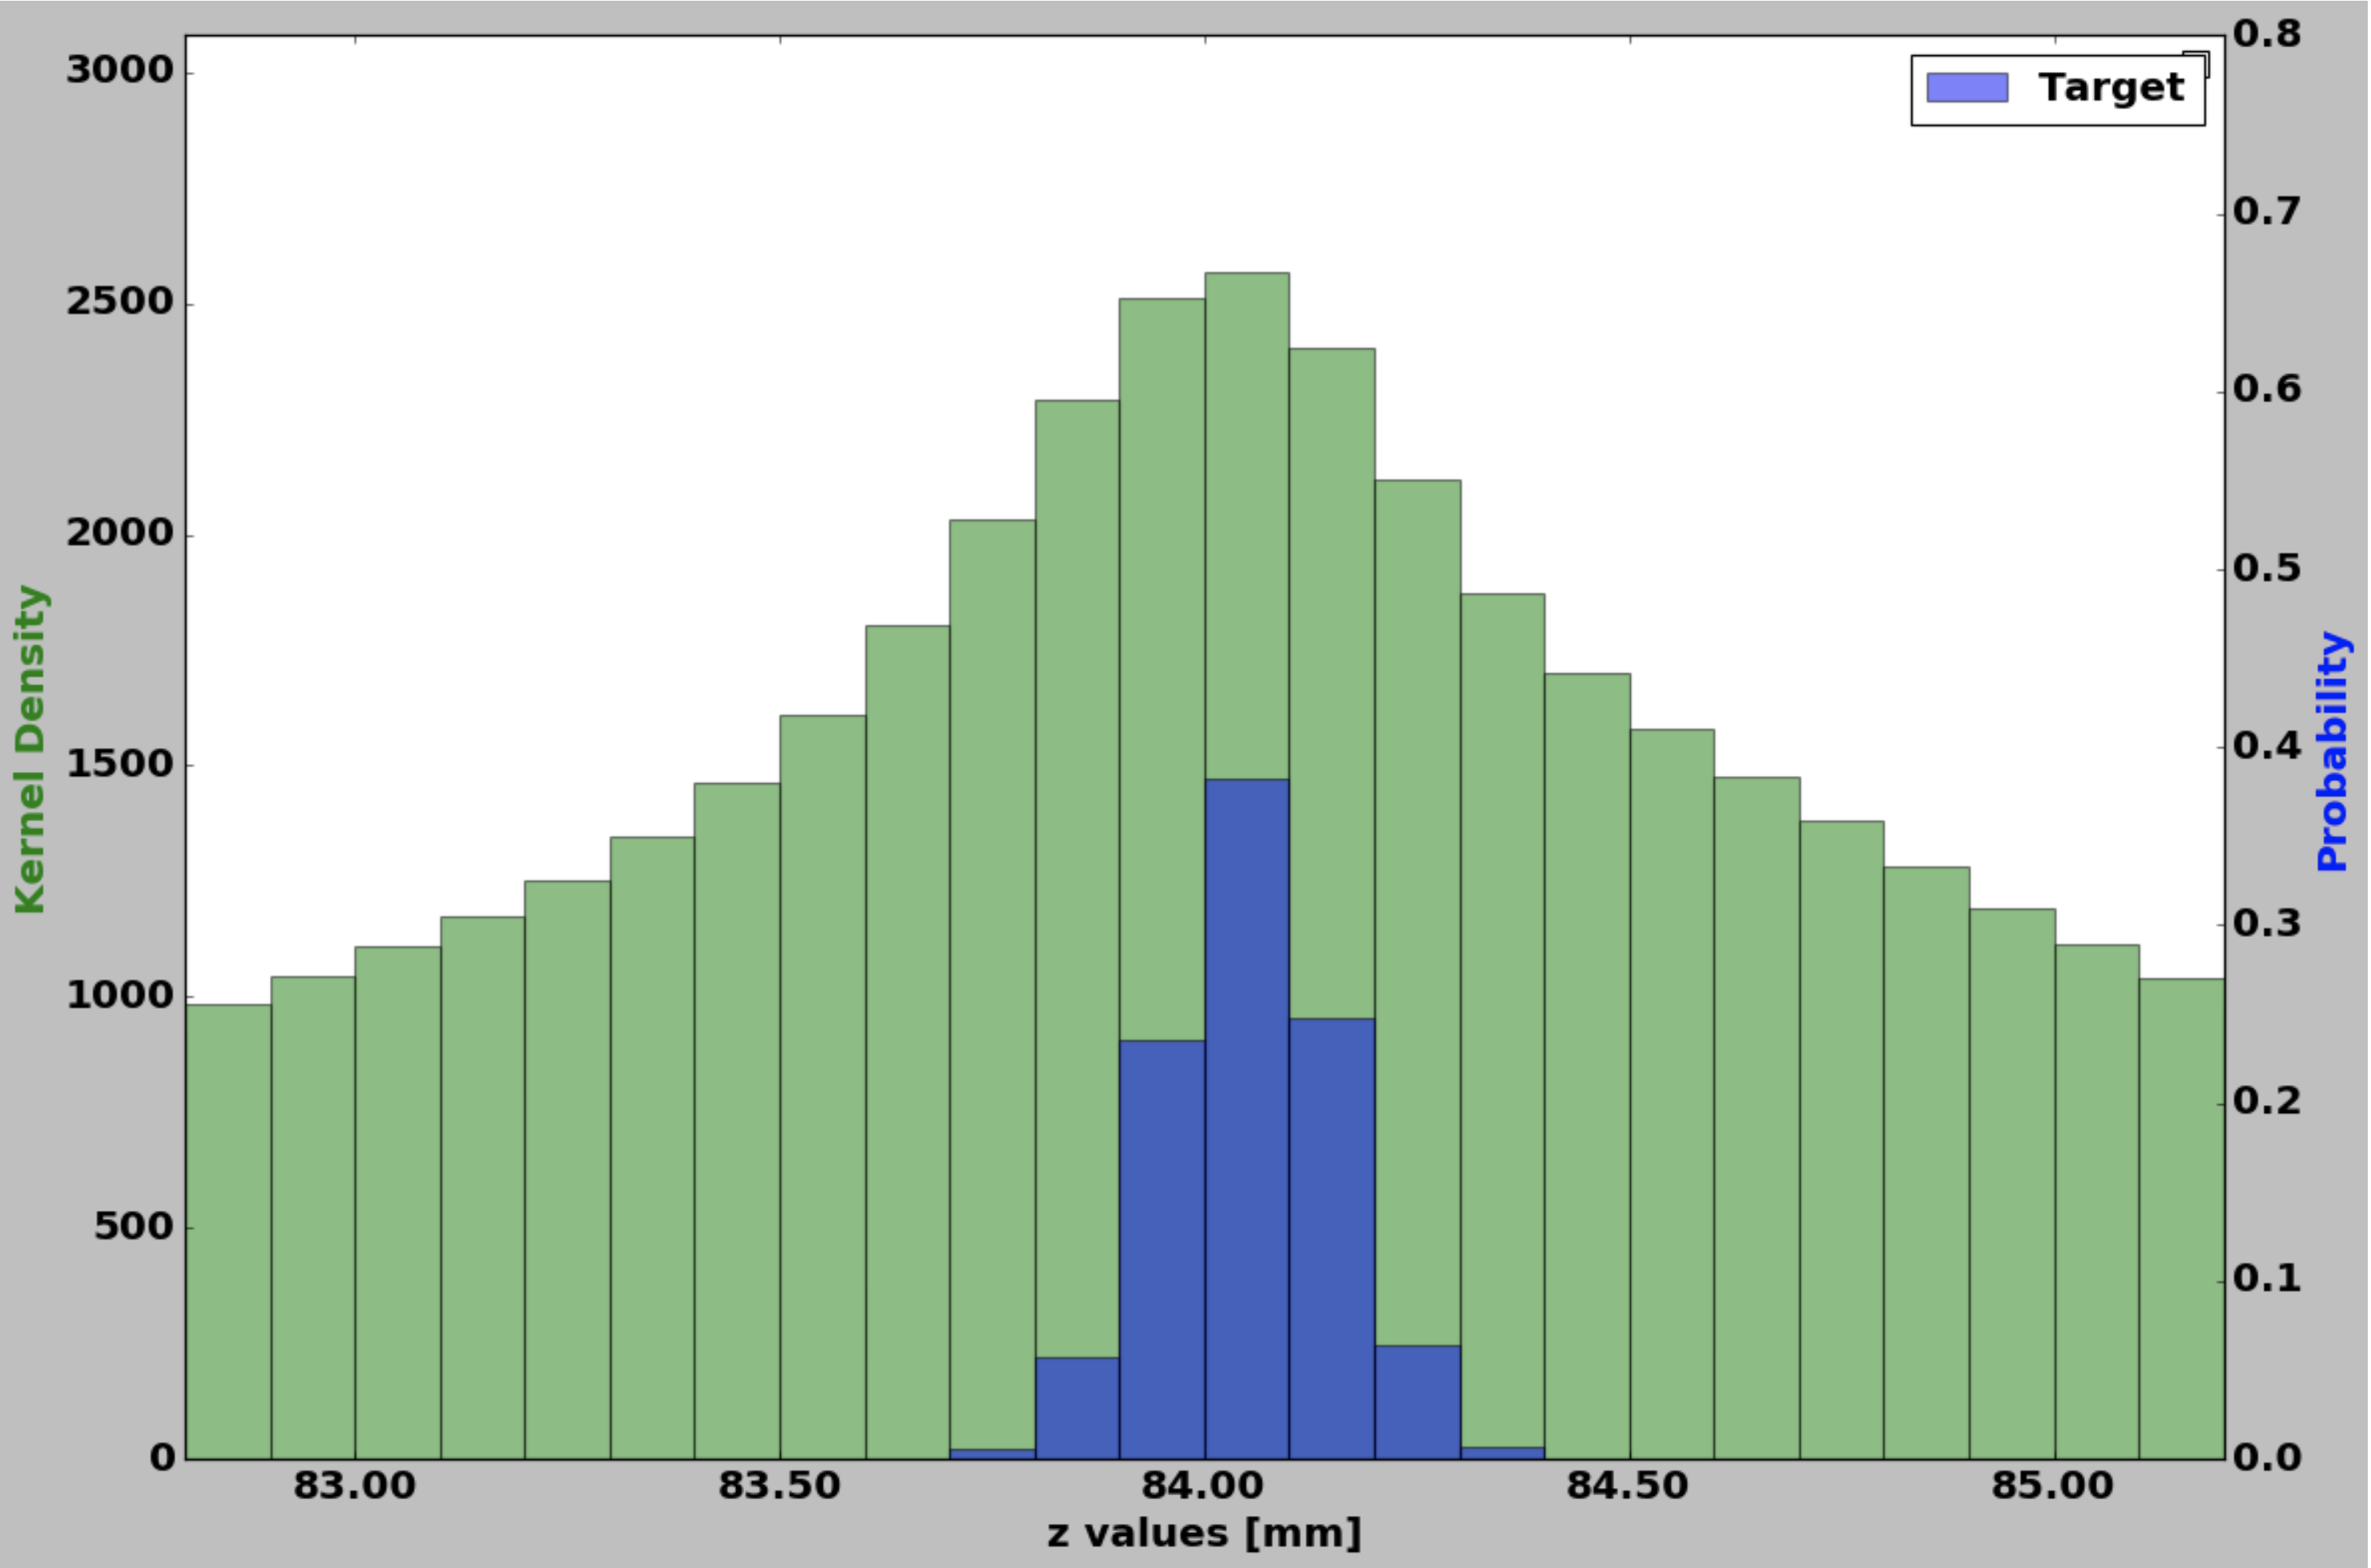
\includegraphics[width=1\textwidth,height=0.45\textwidth, trim=18 0 18 0]{images/T_2_12.png}
    
    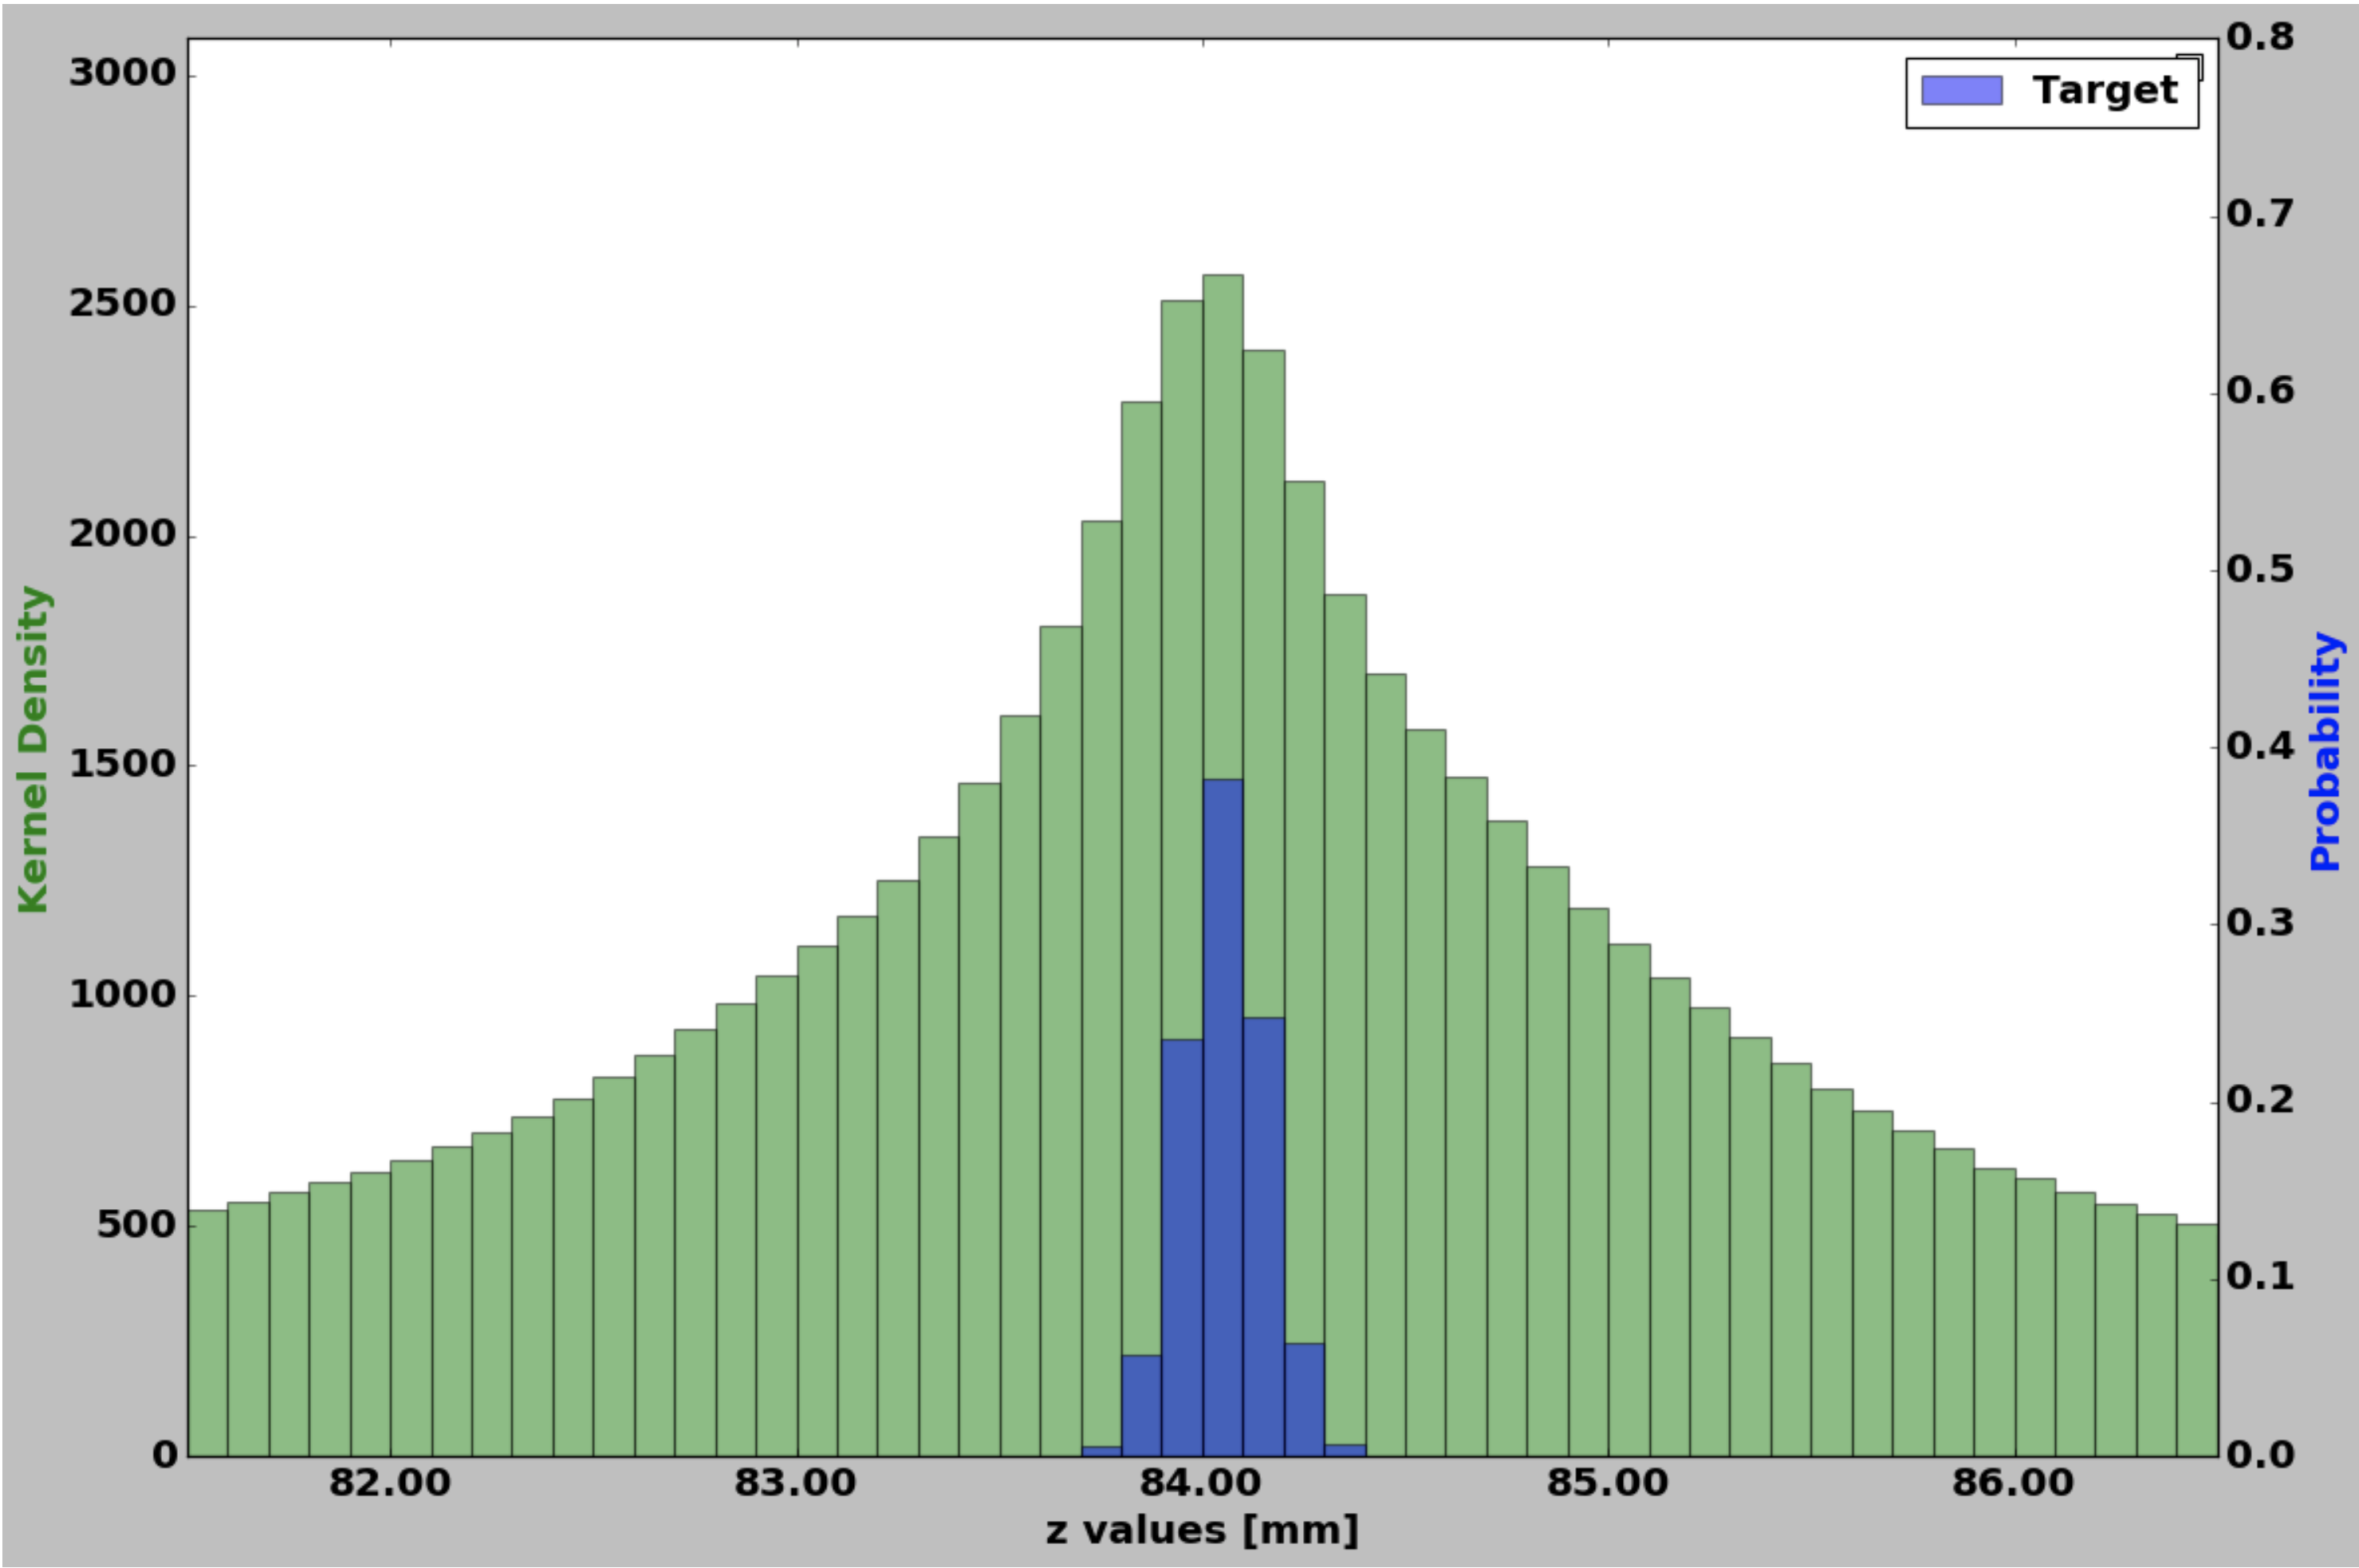
\includegraphics[width=1\textwidth,height=0.45\textwidth, trim=18 0 18 0]{images/T_2_25.png}
  \end{center}
  \end{columns}
\end{frame}
% Part 5: RUI
\subsection{Neural network architecture with two convolutional layers}
\begin{frame}{Neural network architecture}
    \begin{center}
      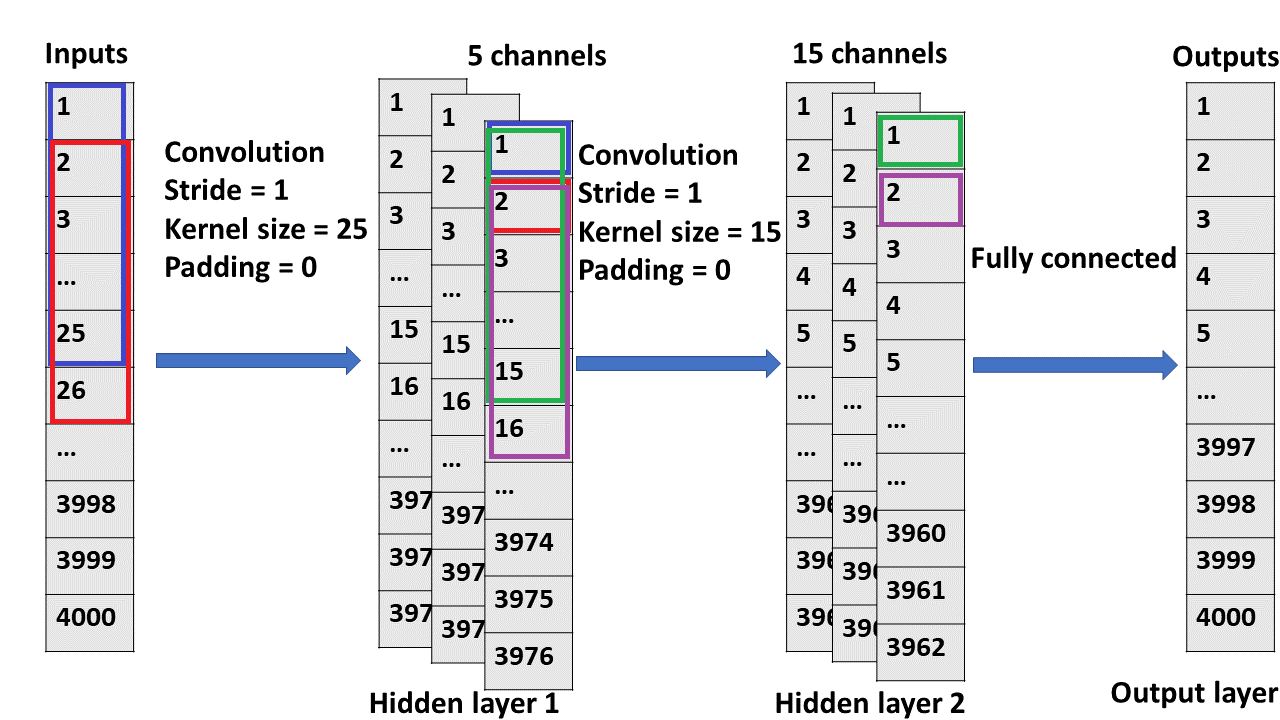
\includegraphics[width=0.75\linewidth, trim=0 30 0 0]{images/CNN_2.png}
   \end{center}
   \begin{itemize}
       \item Activation function for hidden layers: Leaky ReLu
       \item Activation function for output layer: Sigmoid
   \end{itemize}
\end{frame}
\begin{frame}{Activation function}
   \begin{columns}[c]
   % TODO: Swap
        \column{.5\textwidth}
        \begin{center}
            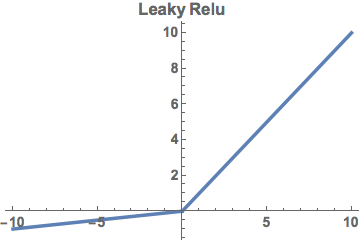
\includegraphics[width=0.8\textwidth]{images/LeakyRelu.png}
            
            Activation function for hidden layers
        \end{center}
    
        \column{.5\textwidth}
        \begin{center}
            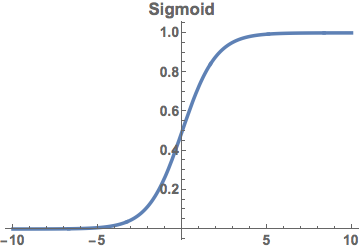
\includegraphics[width=0.8\textwidth]{images/Sigmoid.png}
            
            Activation function for output layer
        \end{center}
  \end{columns}
\end{frame}


% Part 4: MDS
\subsection{Cost Function}
\begin{frame}{Cost Function}
  \begin{columns}[c] 
    \column{0.45\textwidth}
    \begin{block}{Approach}
      \begin{itemize}
         \item 
           Cost function should be similar to Cross-Entropy for $ y \to 0 $,
           $ y \to 1 $;
             $ \color{brickred} \textrm{cost} = - \big (y \ln \hat{y} + (1-y) \ln (1 - \hat{y}) \big )  $
         \item
          Should be symmetric with respect to  $ r = ( \hat y/y  )$ \& $ 1/r $
     \end{itemize}
    \end{block}
    \begin{block}{Sum Over Bins}
      \begin{equation}
        \color{brickred}
        r_i \equiv (\hat{y_i} + \epsilon)/ (y_i + \epsilon)
      \end{equation}
      \vspace{-.9em}
      \begin{equation}
        \color{brickred}
        z_i \equiv \frac{2 \, r_i }{r_i + 1/r_i}
      \end{equation}
      \vspace{-.4em}
      \begin{equation}
        \color{brickred}
        \textrm{our cost} = \sum_{\textrm{bins}} {- \ln{z_i}}
      \end{equation}
      \vspace{-.7em}
    \end{block}
    \column{0.6\textwidth}
      \centering
      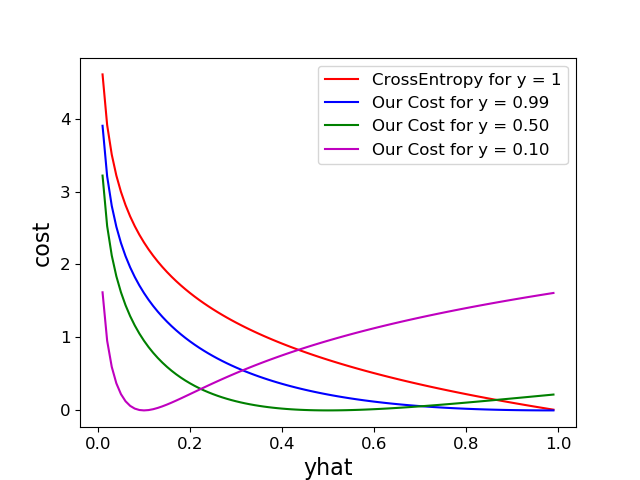
\includegraphics[width=1.0\linewidth]{images/CostPlot.png}
      \end{columns}
\end{frame}


\section{Results}
% Part 6: RUI
\subsection{Cost plot}
\begin{frame}{Cost, efficiency, and false positive rate: 2 convolutionial layers}
   \centering
   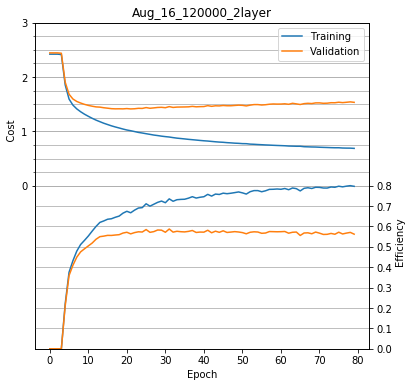
\includegraphics[width=0.45\linewidth]{images/CNN_2Layer_Cost.png}
   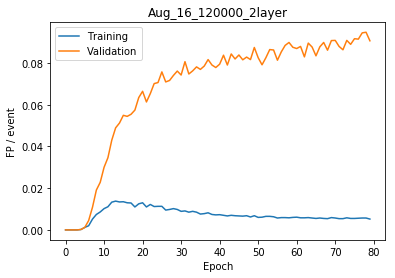
\includegraphics[width=0.45\linewidth]{images/CNN_2Layer_FalsePositive.png}

\end{frame}

\begin{frame}{Cost, efficiency, and false positive rate: 3 convolutionial layers}
   \centering
   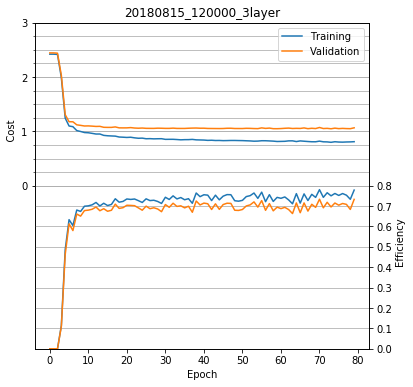
\includegraphics[width=0.45\linewidth]{images/CNN_3Layer_Cost.png}
   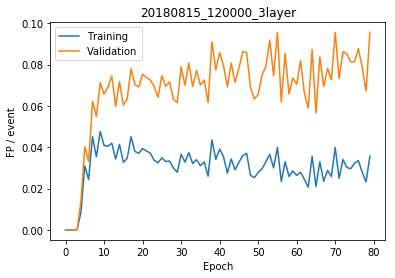
\includegraphics[width=0.45\linewidth]{images/CNN_3Layer_FalsePositive.png}

\end{frame}
\subsection{Prediction plots}

\begin{frame}{Compare Predictions with Targets (3 convolutional layers)}
  \begin{columns}[c]
    \column{.5\textwidth}
        \begin{center}
            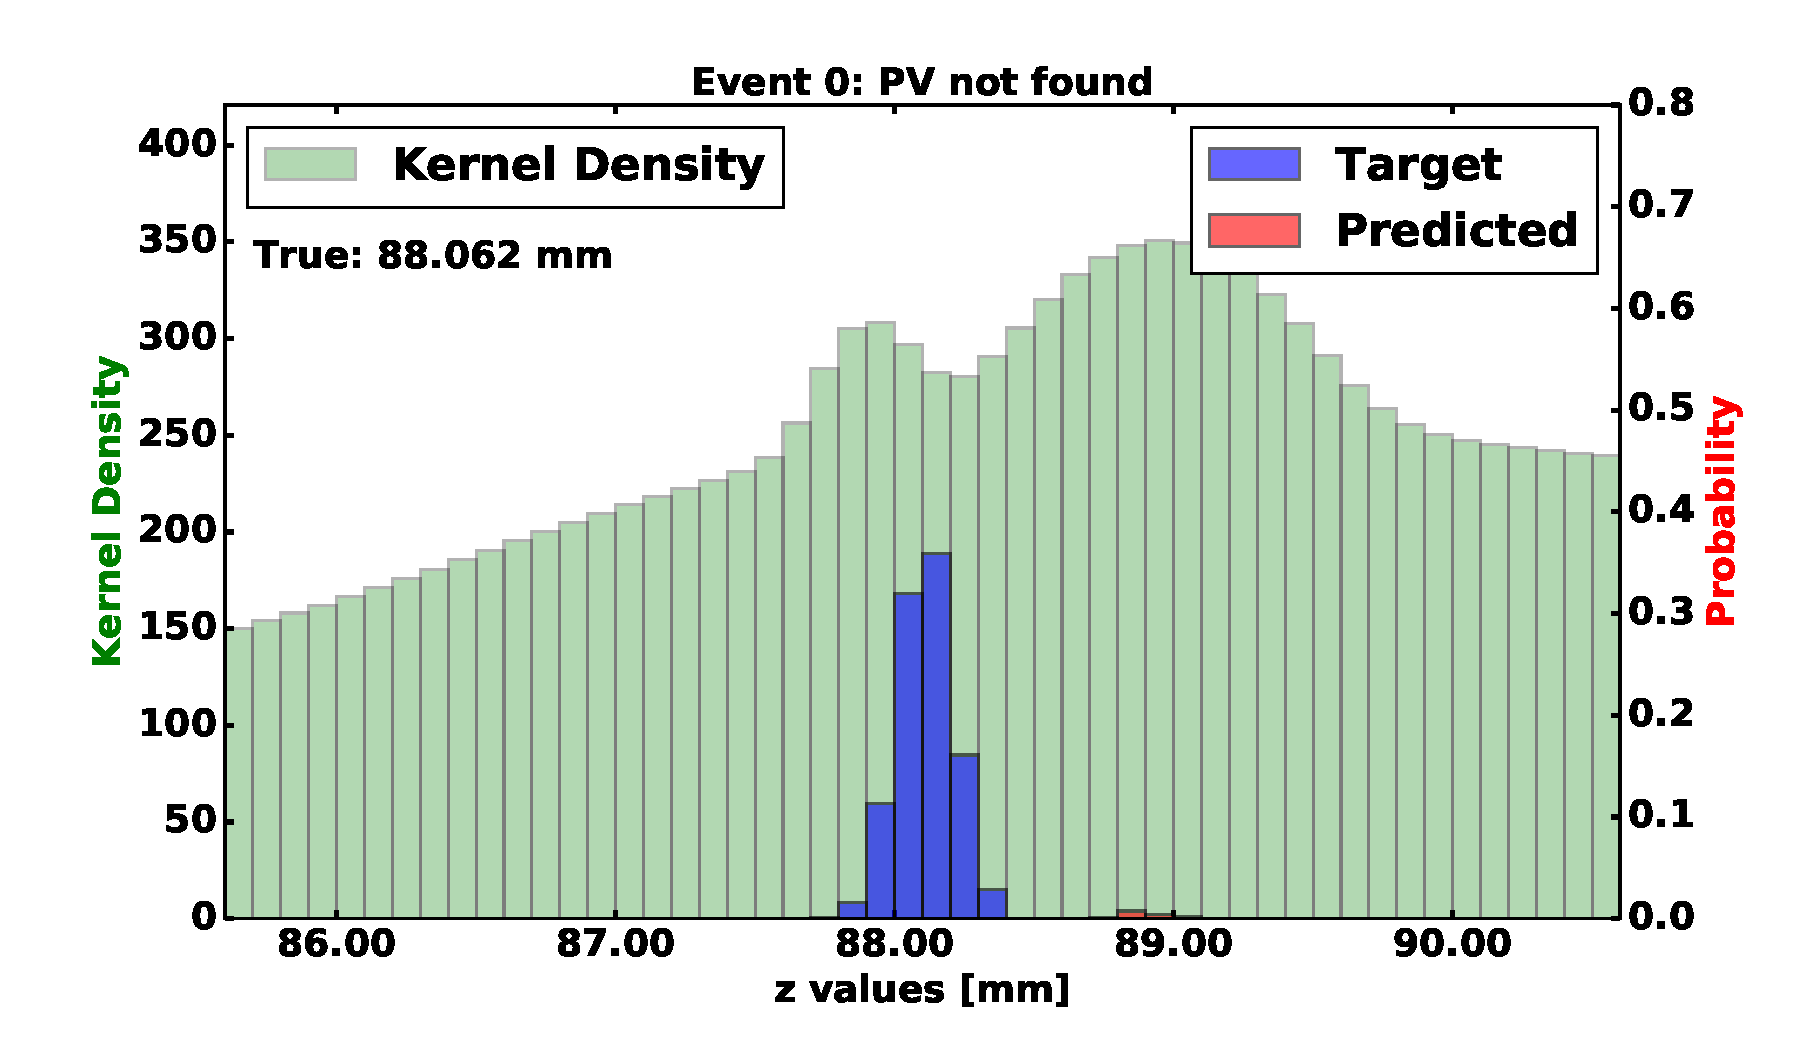
\includegraphics[width=1\textwidth,height=0.45\textwidth, trim=18 0 18 0]{images/120000_3layer_00.pdf}
    
            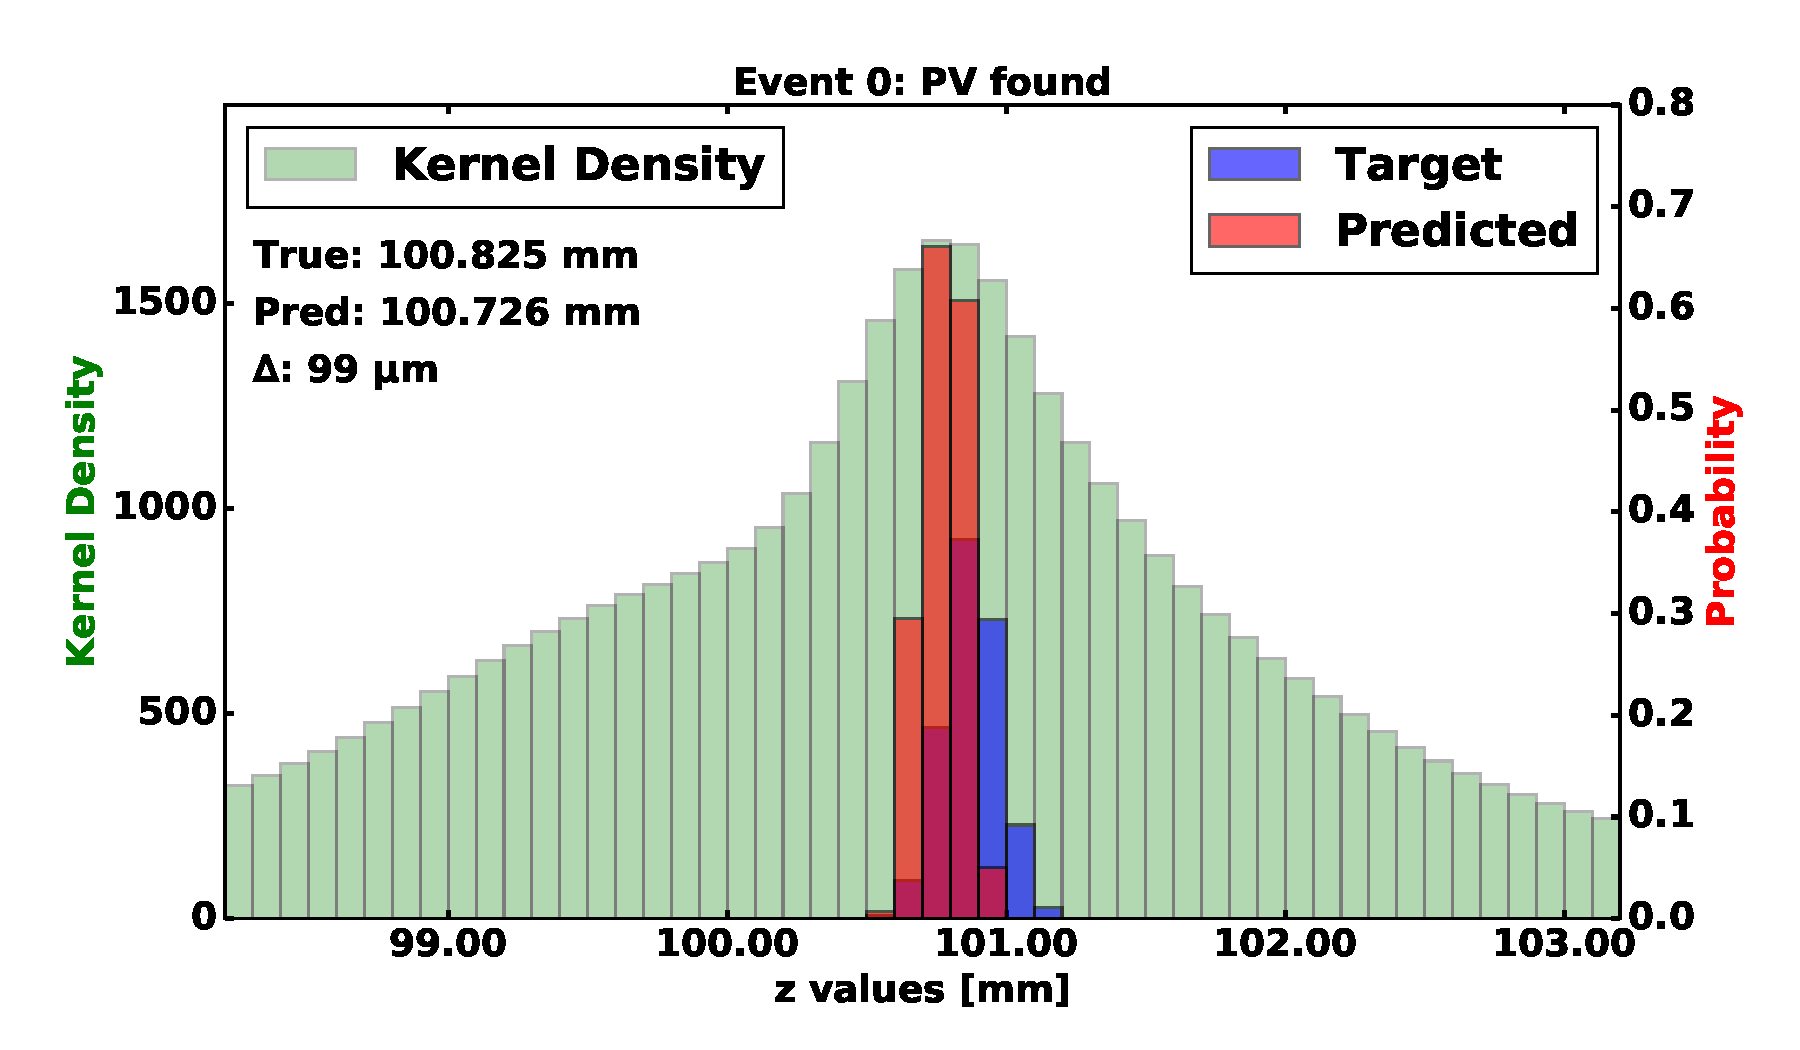
\includegraphics[width=1\textwidth, height=0.45\textwidth,trim=18 0 18 0]{images/120000_3layer_01.pdf}

        \end{center}
    \column{.5\textwidth}
        \begin{center}
           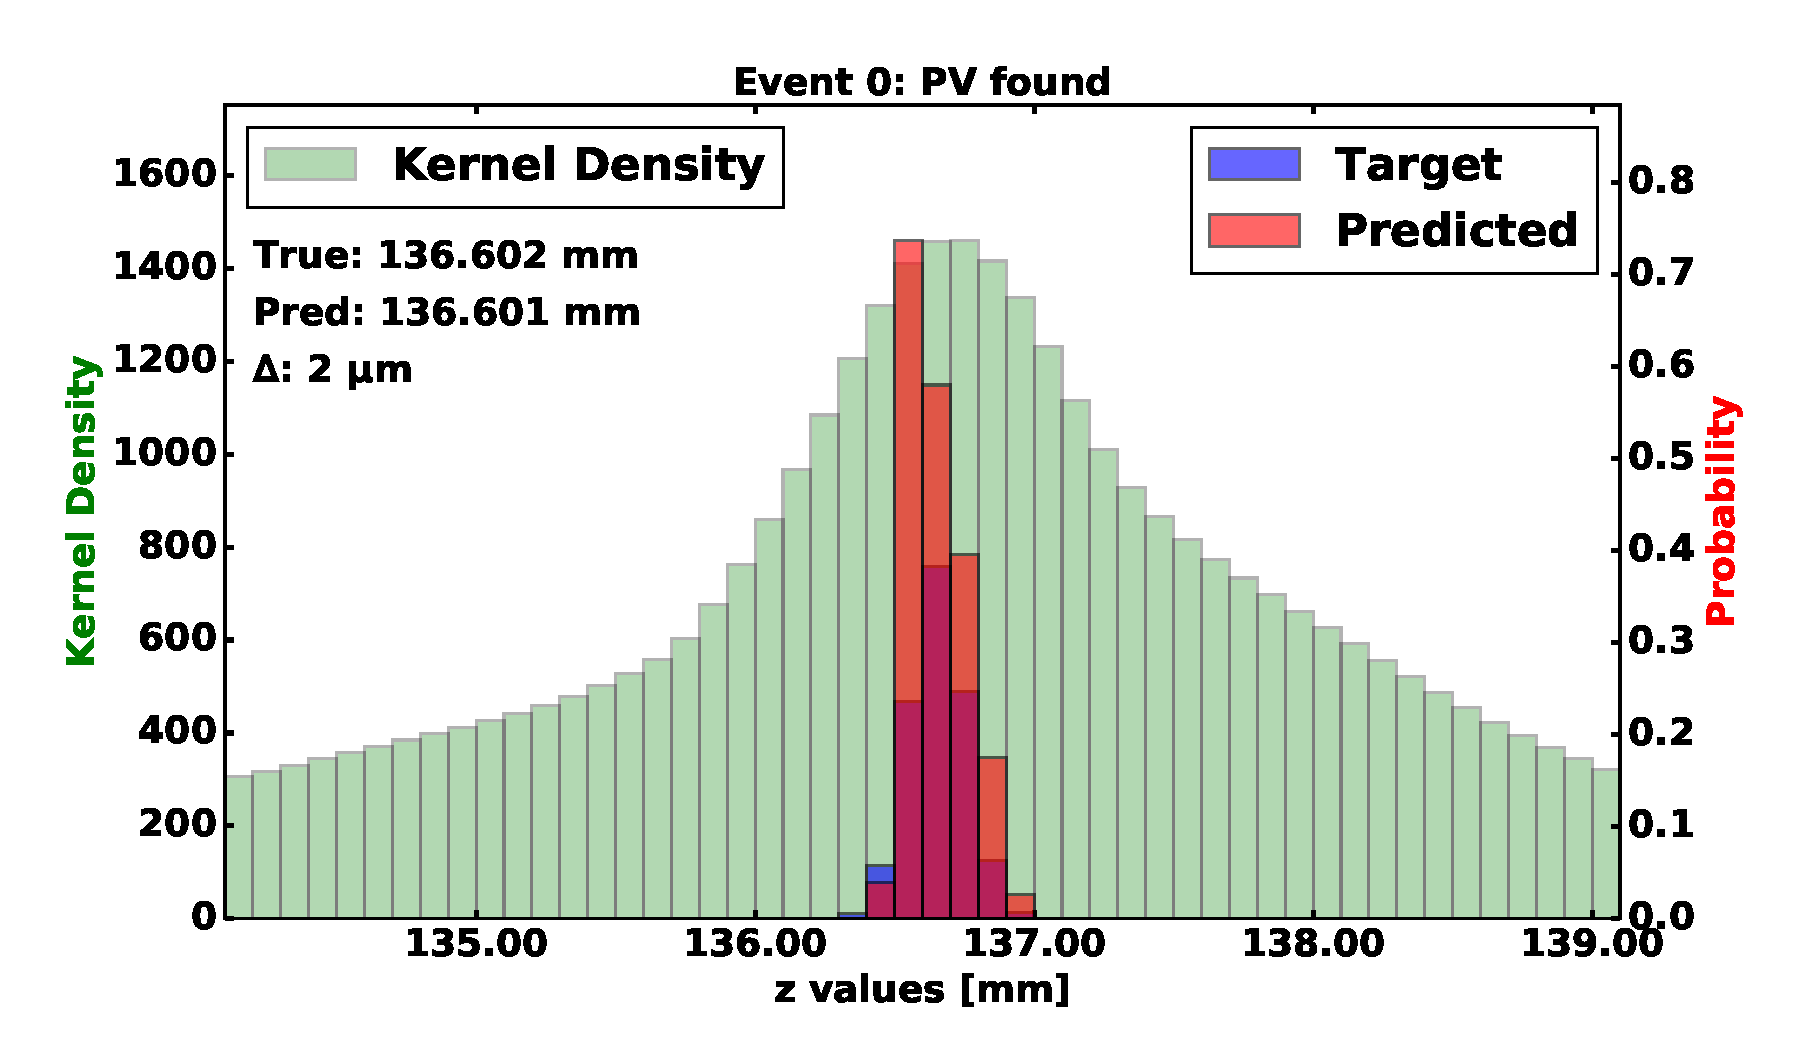
\includegraphics[width=1\textwidth, height=0.45\textwidth, trim=18 0 18 0]{images/120000_3layer_02.pdf}
    
           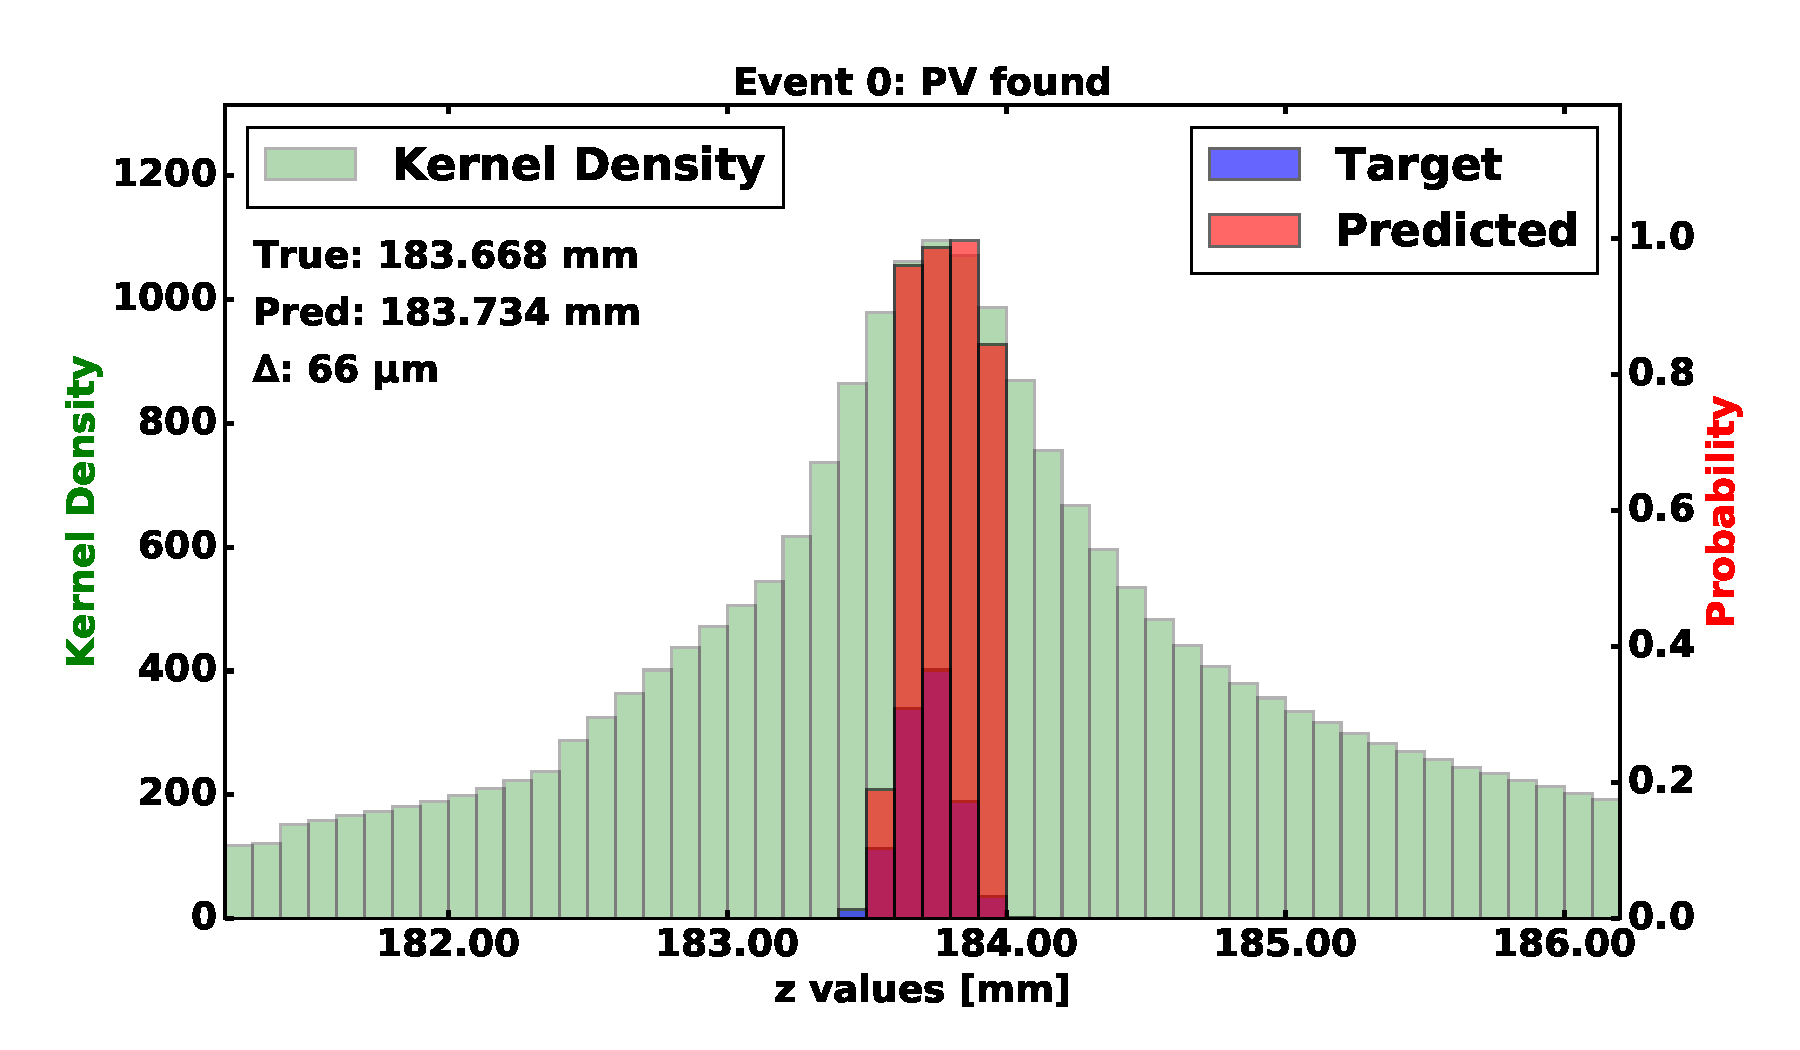
\includegraphics[width=1\textwidth, height=0.45\textwidth, trim=18 0 18 0]{images/120000_3layer_03.pdf}
       \end{center}
  \end{columns}
\end{frame}

\begin{frame}{Compare Predictions with Targets (3 convolutional layers)}
  \begin{columns}[c]
    \column{.5\textwidth}
        \begin{center}
            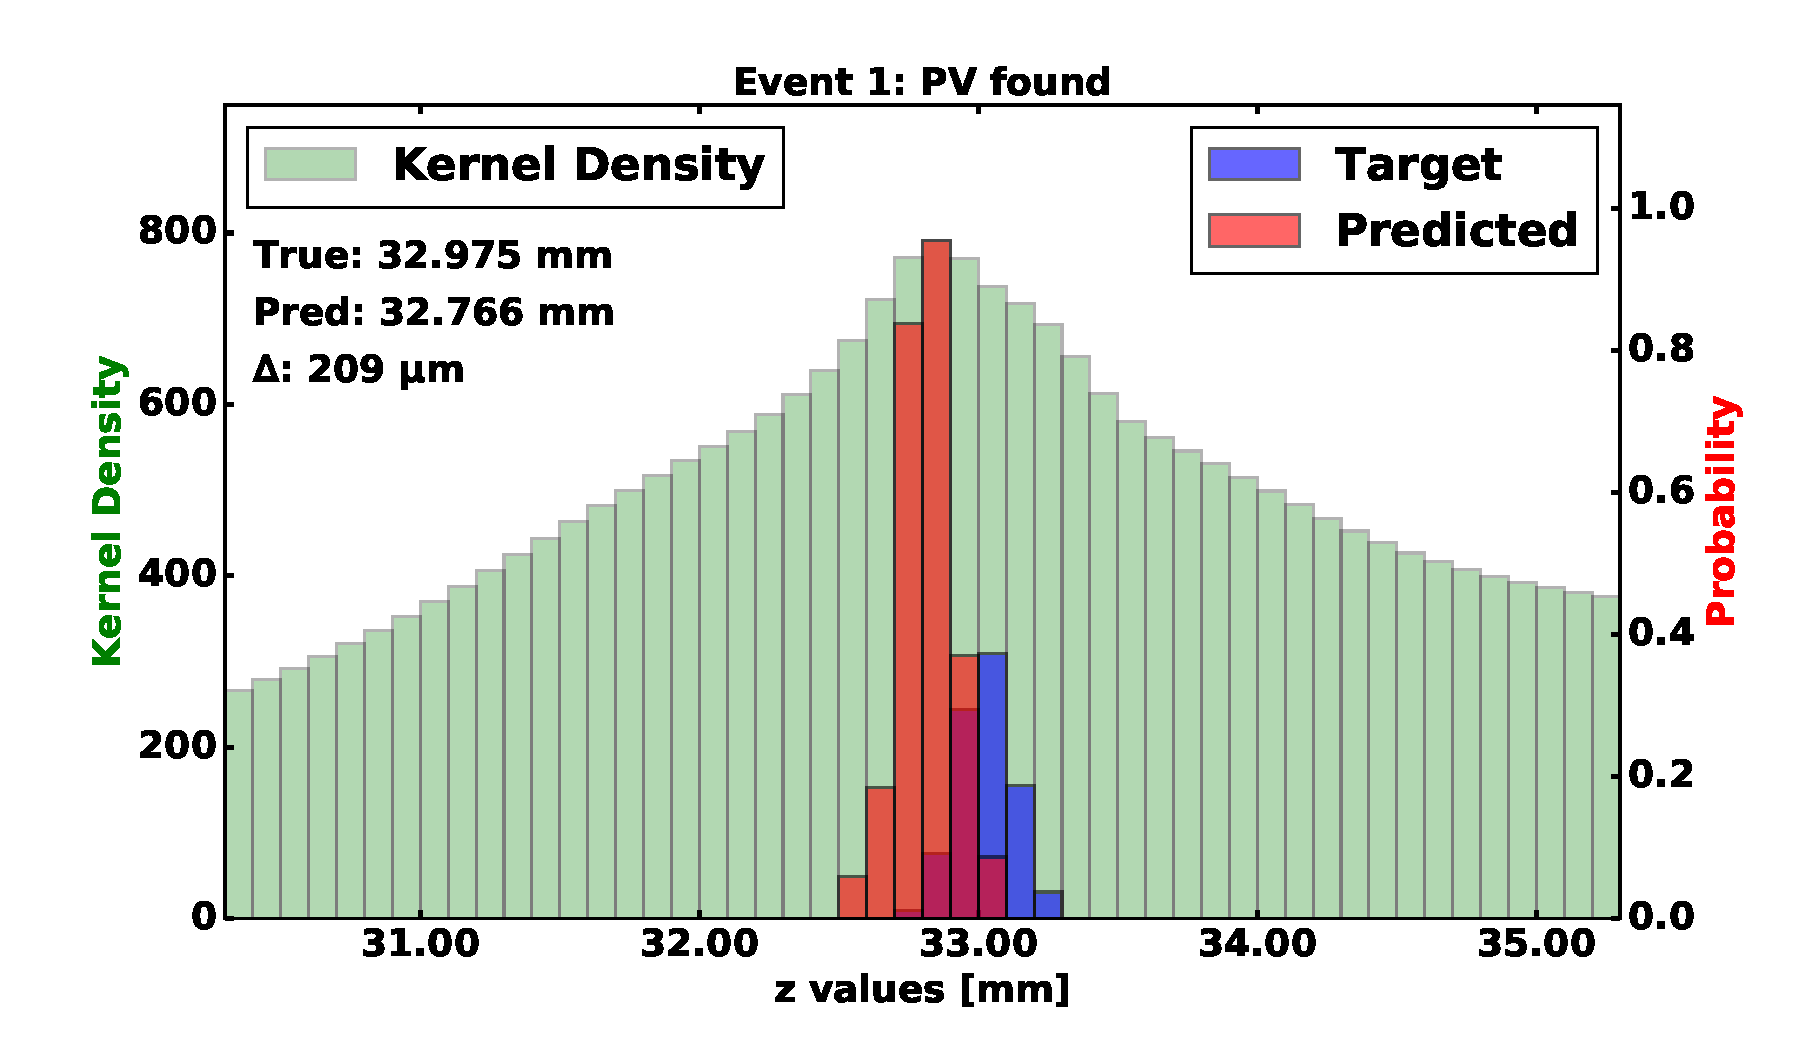
\includegraphics[width=1\textwidth,height=0.45\textwidth, trim=18 0 18 0]{images/120000_3layer_04.pdf}
    
            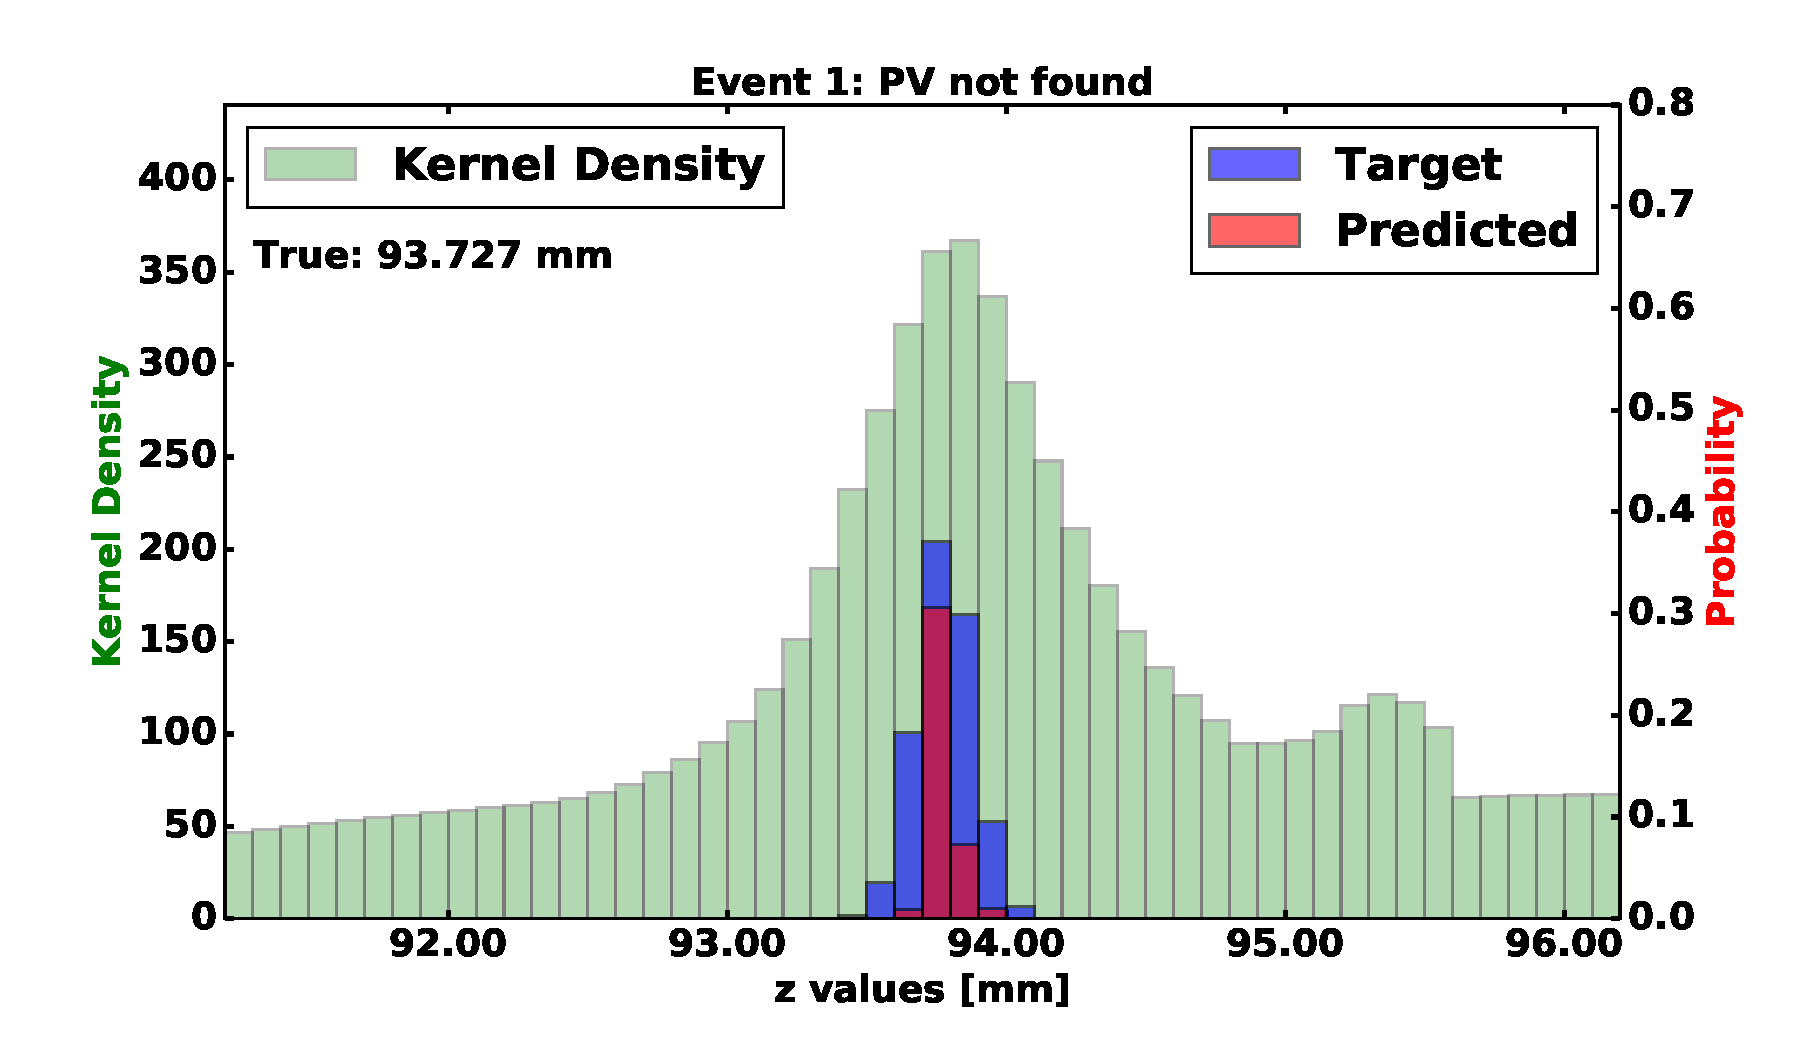
\includegraphics[width=1\textwidth, height=0.45\textwidth,trim=18 0 18 0]{images/120000_3layer_05.pdf}

        \end{center}
    \column{.5\textwidth}
        \begin{center}
           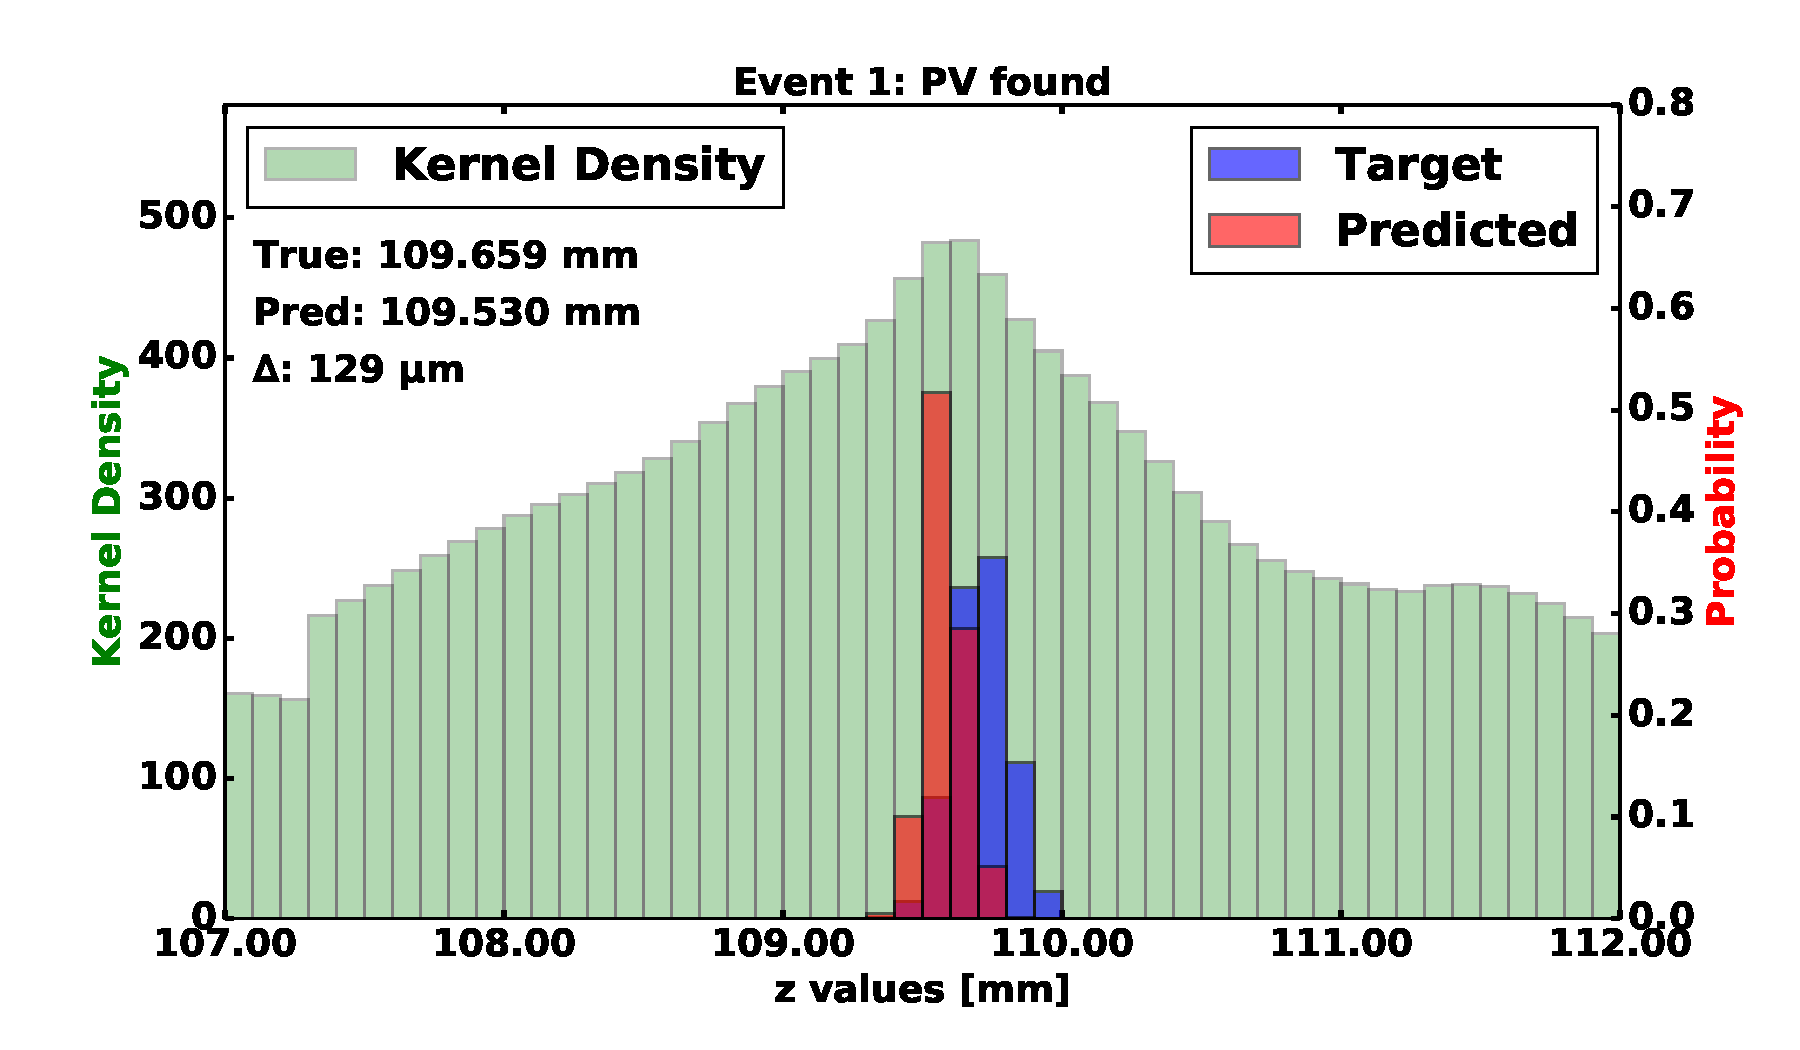
\includegraphics[width=1\textwidth, height=0.45\textwidth, trim=18 0 18 0]{images/120000_3layer_06.pdf}
    
           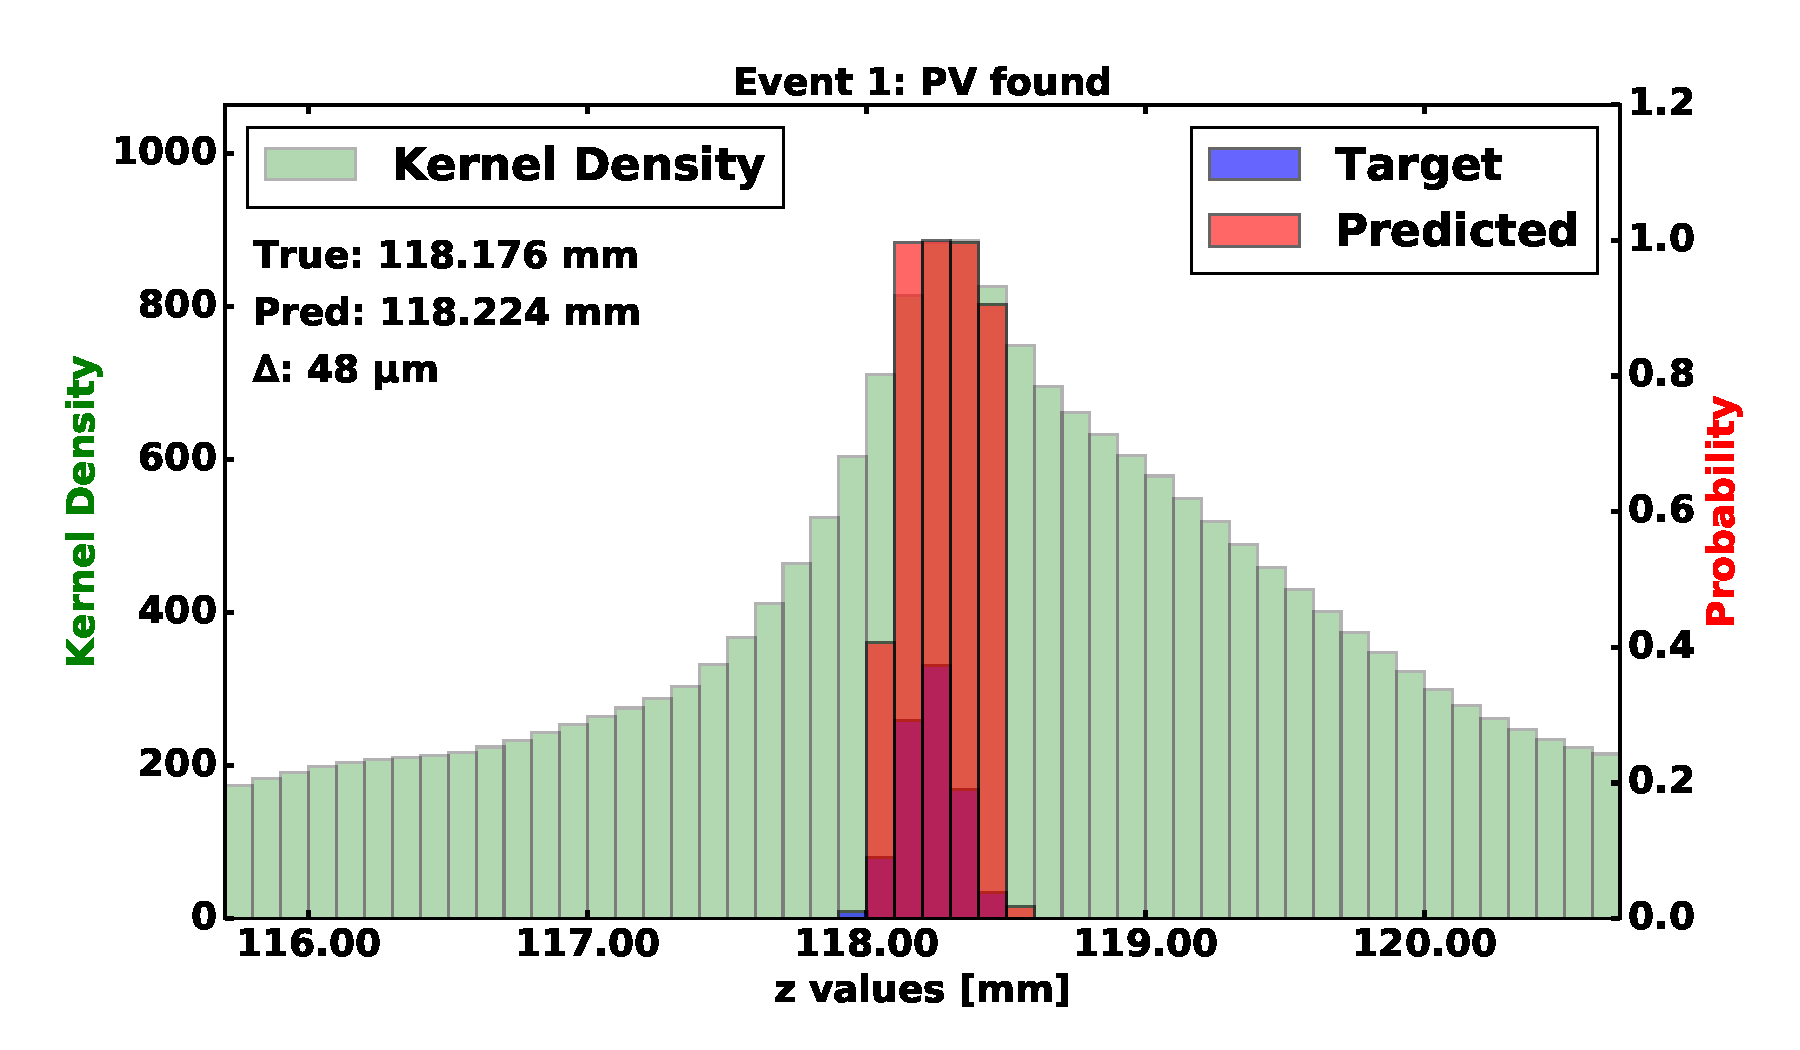
\includegraphics[width=1\textwidth, height=0.45\textwidth, trim=18 0 18 0]{images/120000_3layer_07.pdf}
       \end{center}
  \end{columns}
\end{frame}

\begin{frame}{Compare Predictions with Targets (3 convolutional layers)}
  \begin{columns}[c]
    \column{.5\textwidth}
        \begin{center}
            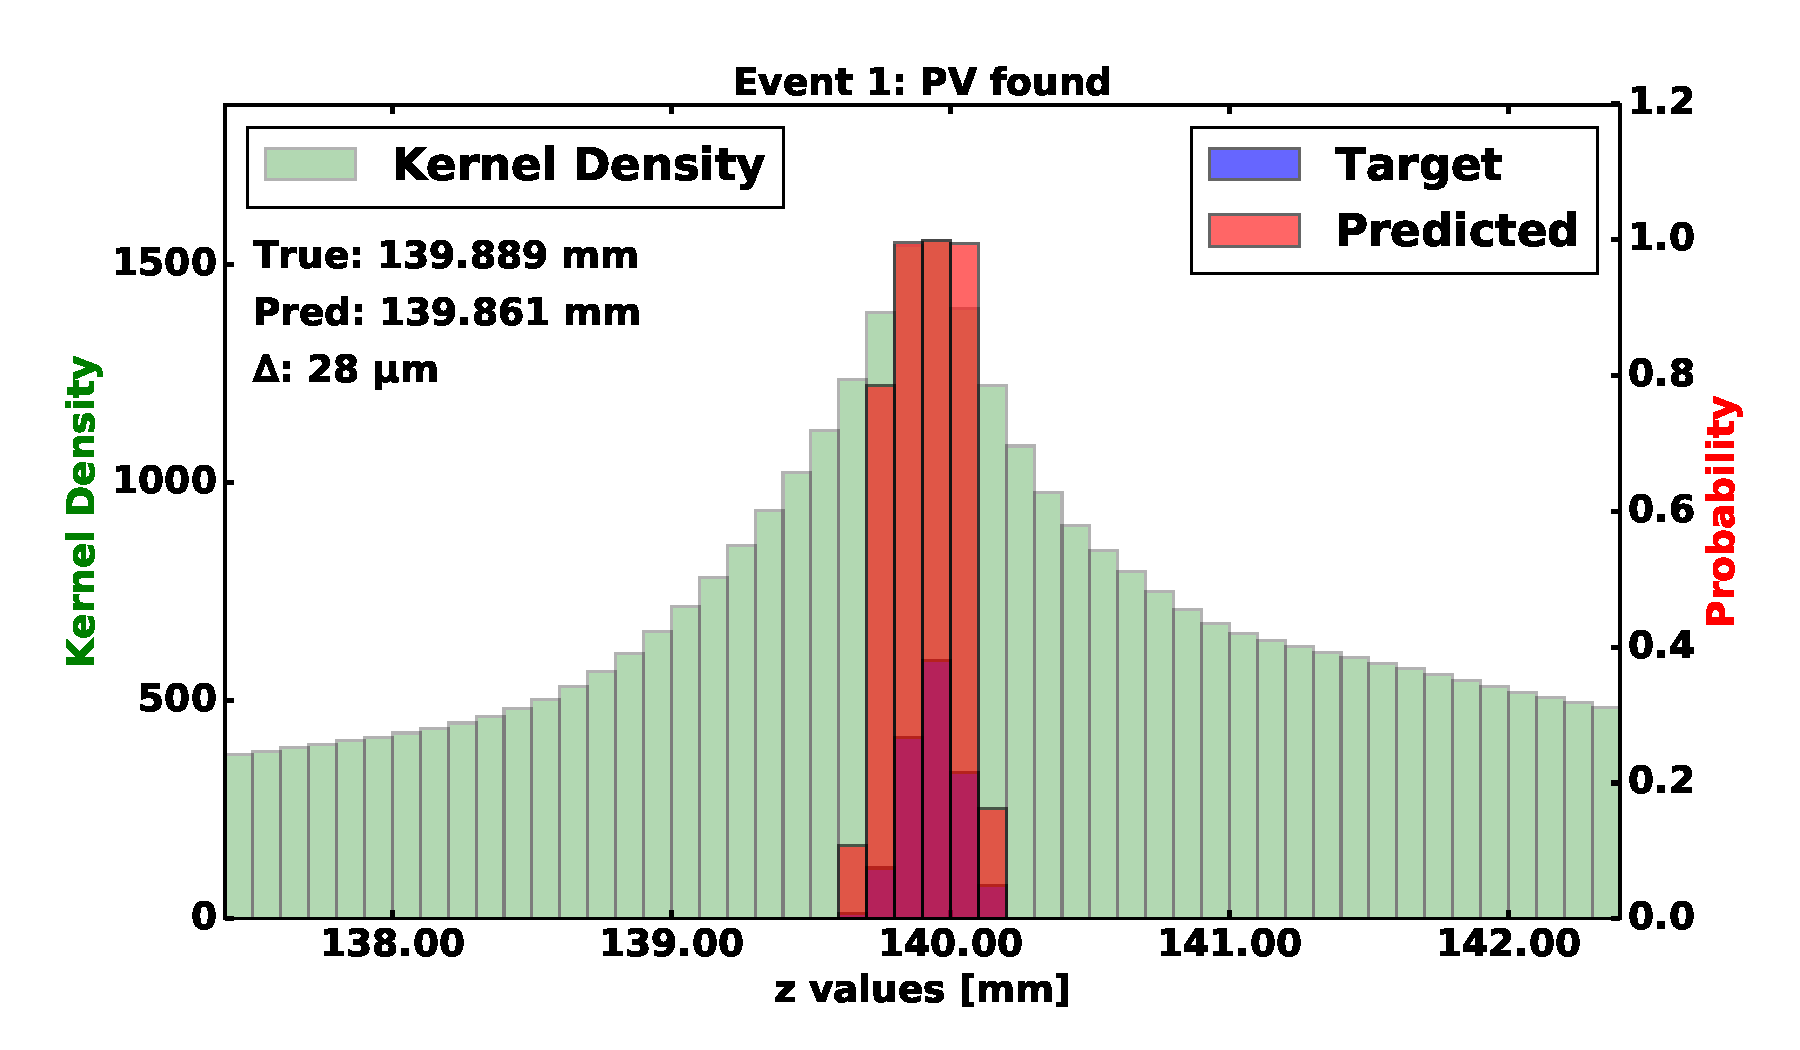
\includegraphics[width=1\textwidth,height=0.45\textwidth, trim=18 0 18 0]{images/120000_3layer_08.pdf}
    
            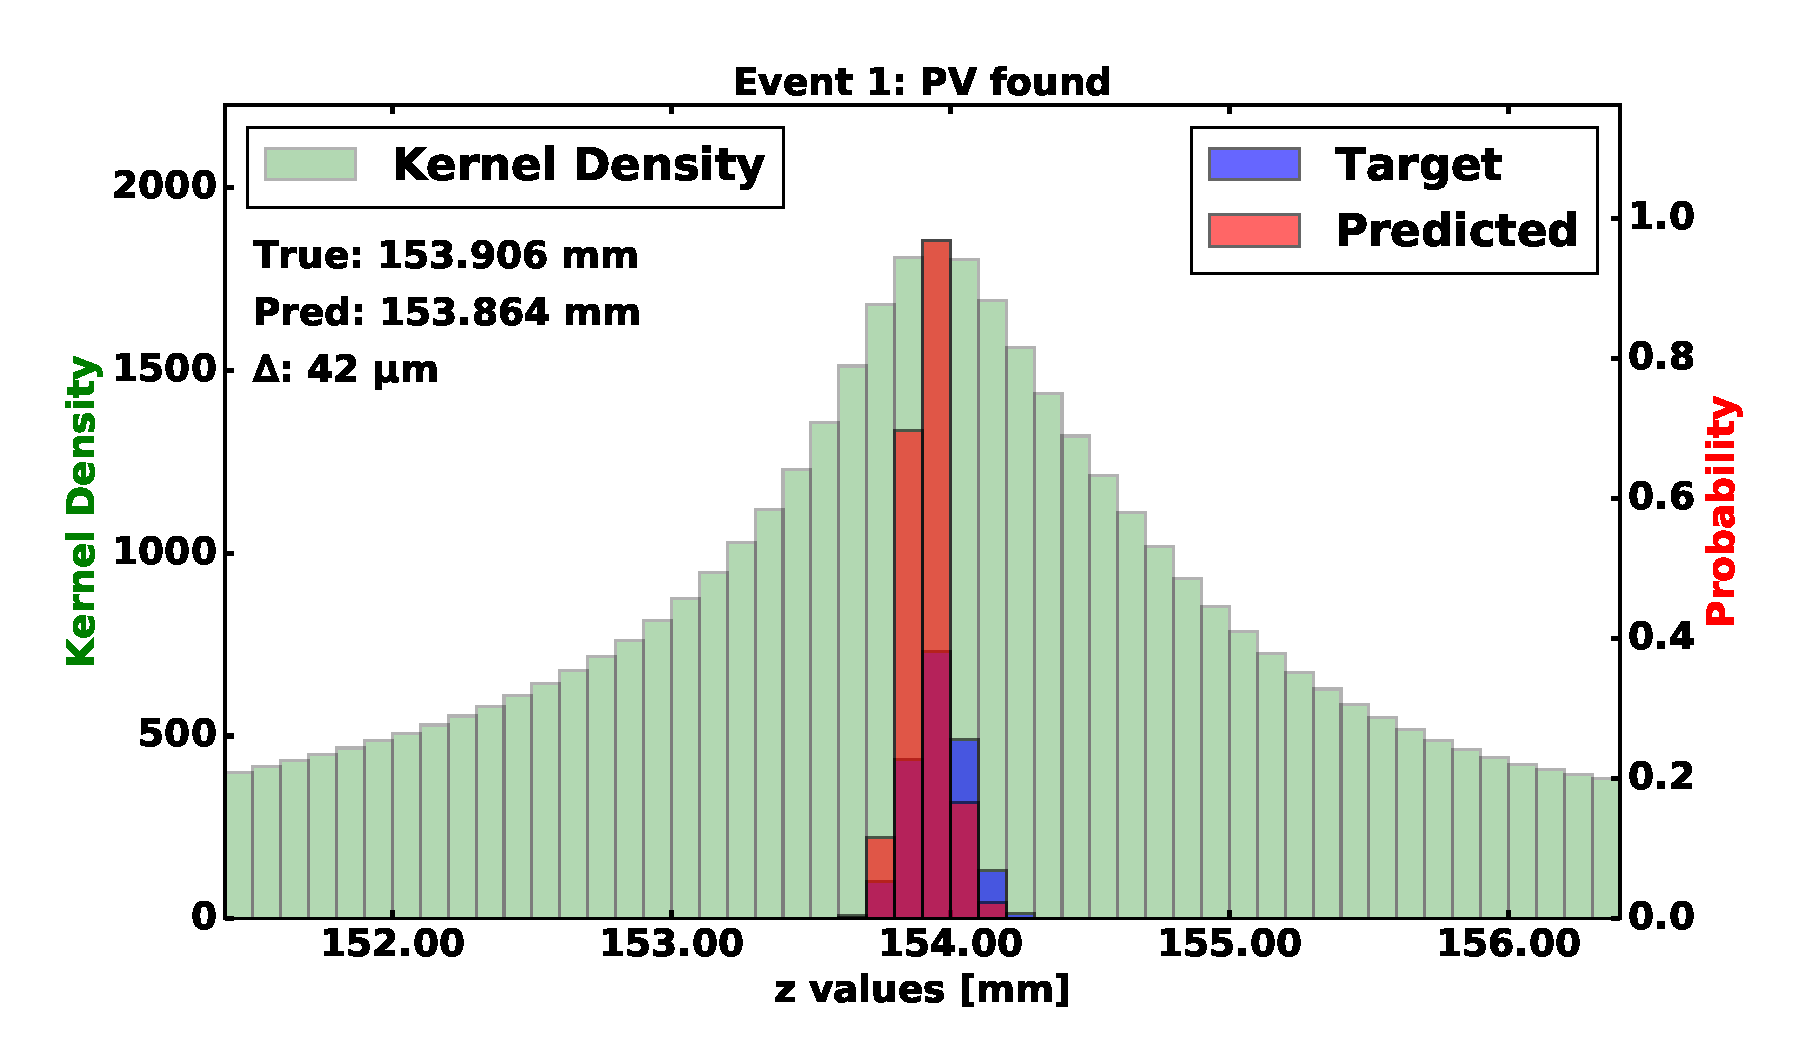
\includegraphics[width=1\textwidth, height=0.45\textwidth,trim=18 0 18 0]{images/120000_3layer_09.pdf}

        \end{center}
    \column{.5\textwidth}
        \begin{center}
           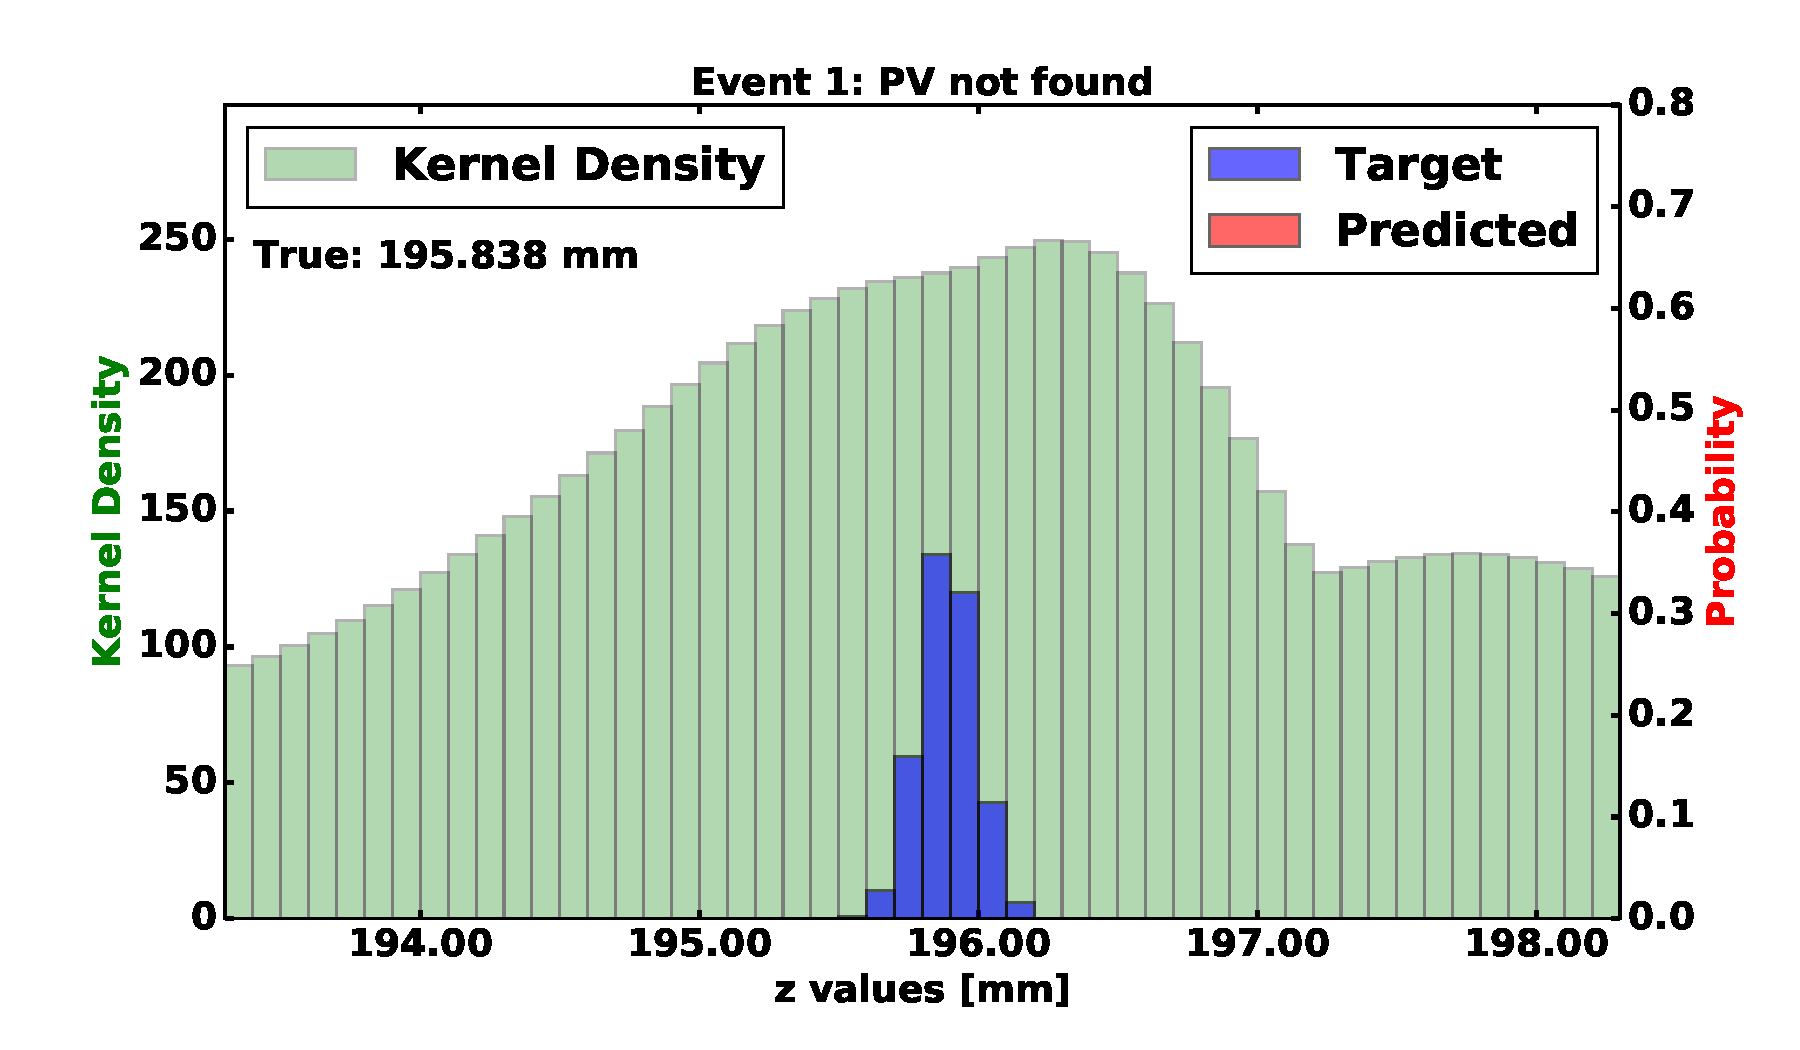
\includegraphics[width=1\textwidth, height=0.45\textwidth, trim=18 0 18 0]{images/120000_3layer_10.pdf}
    
           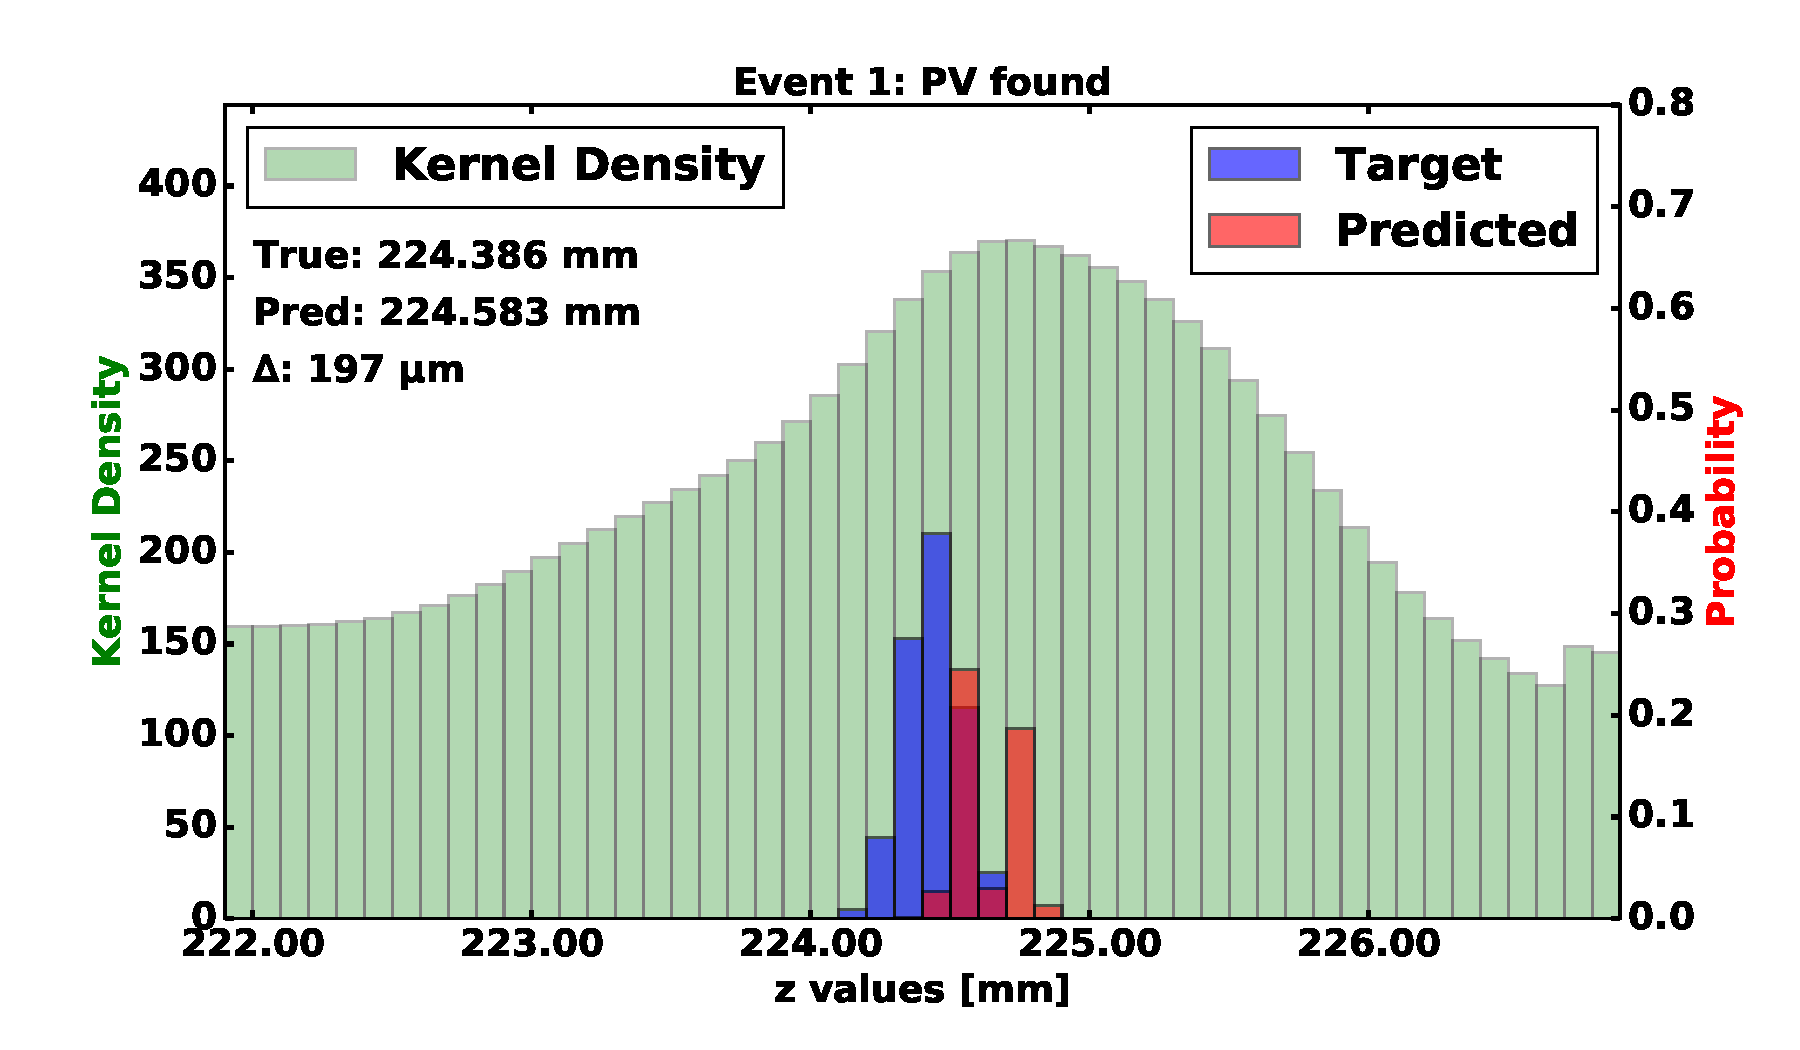
\includegraphics[width=1\textwidth, height=0.45\textwidth, trim=18 0 18 0]{images/120000_3layer_11.pdf}
       \end{center}
  \end{columns}
\end{frame}

\begin{frame}{Compare Predictions with Targets (3 convolutional layers)}
  \begin{columns}[c]
    \column{.5\textwidth}
        \begin{center}
            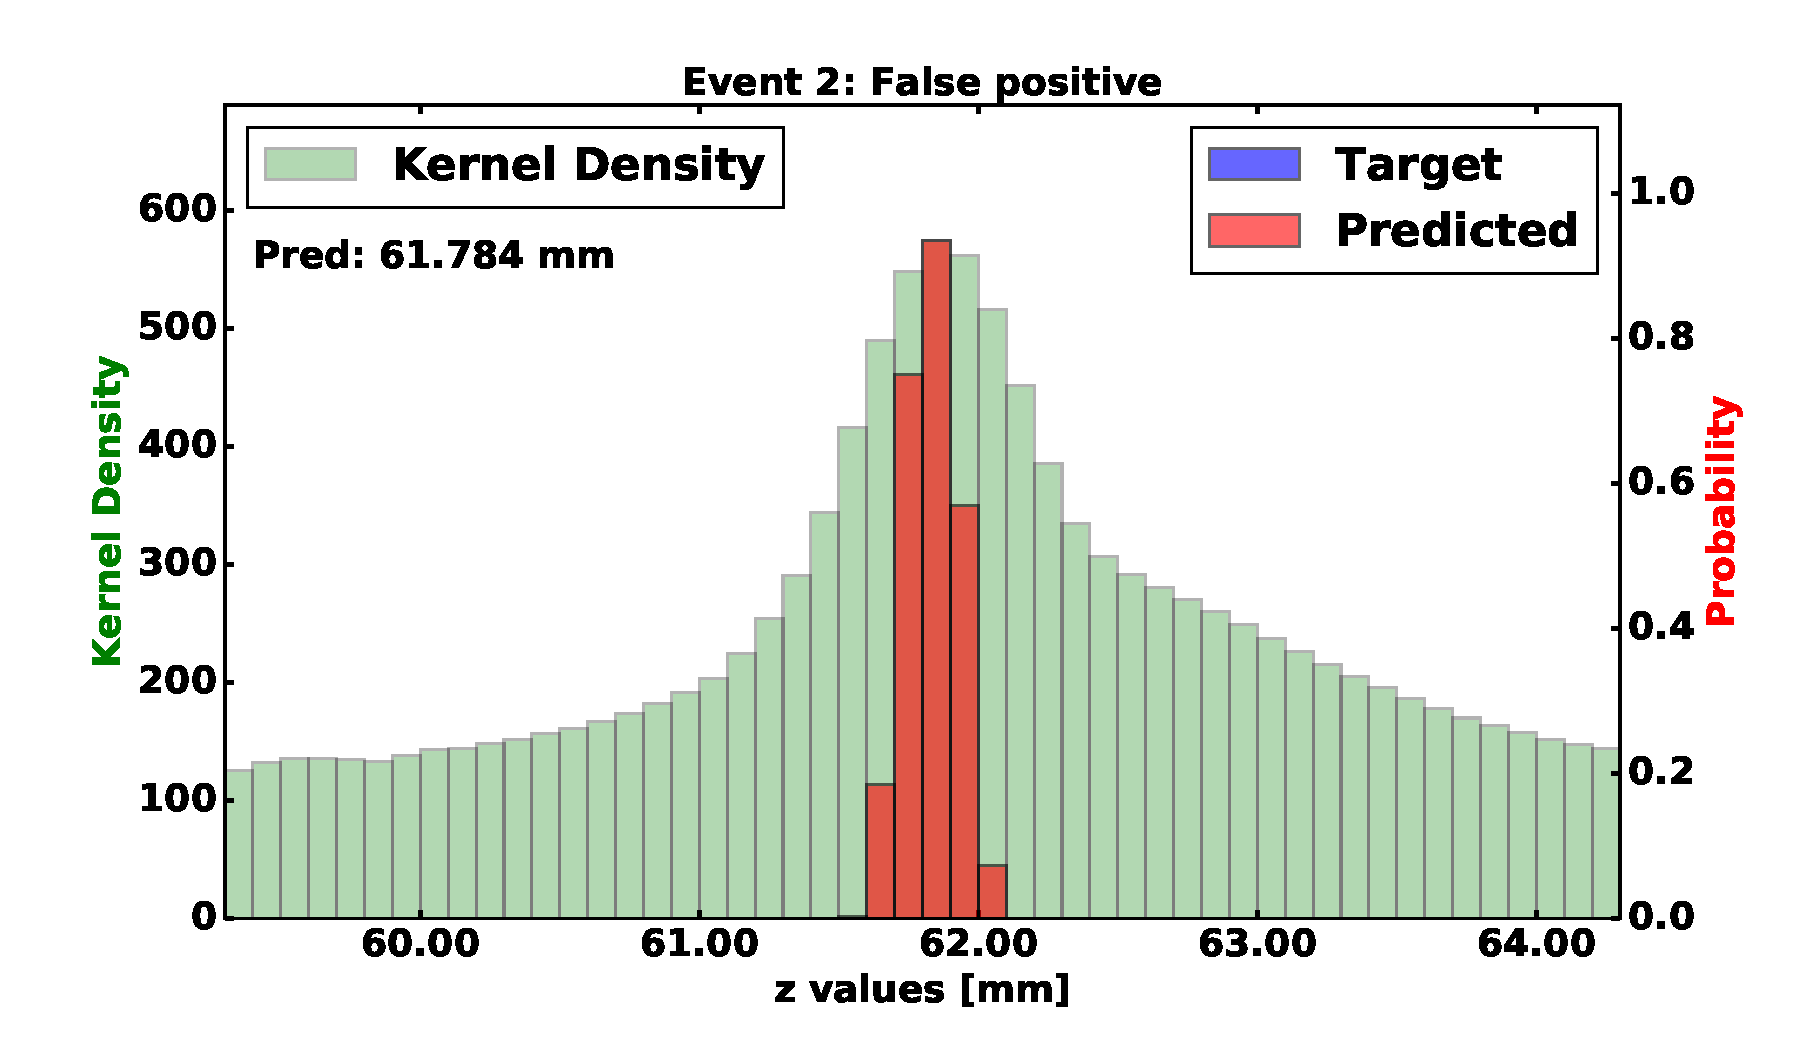
\includegraphics[width=1\textwidth,height=0.45\textwidth, trim=18 0 18 0]{images/120000_3layer_12.pdf}
    
            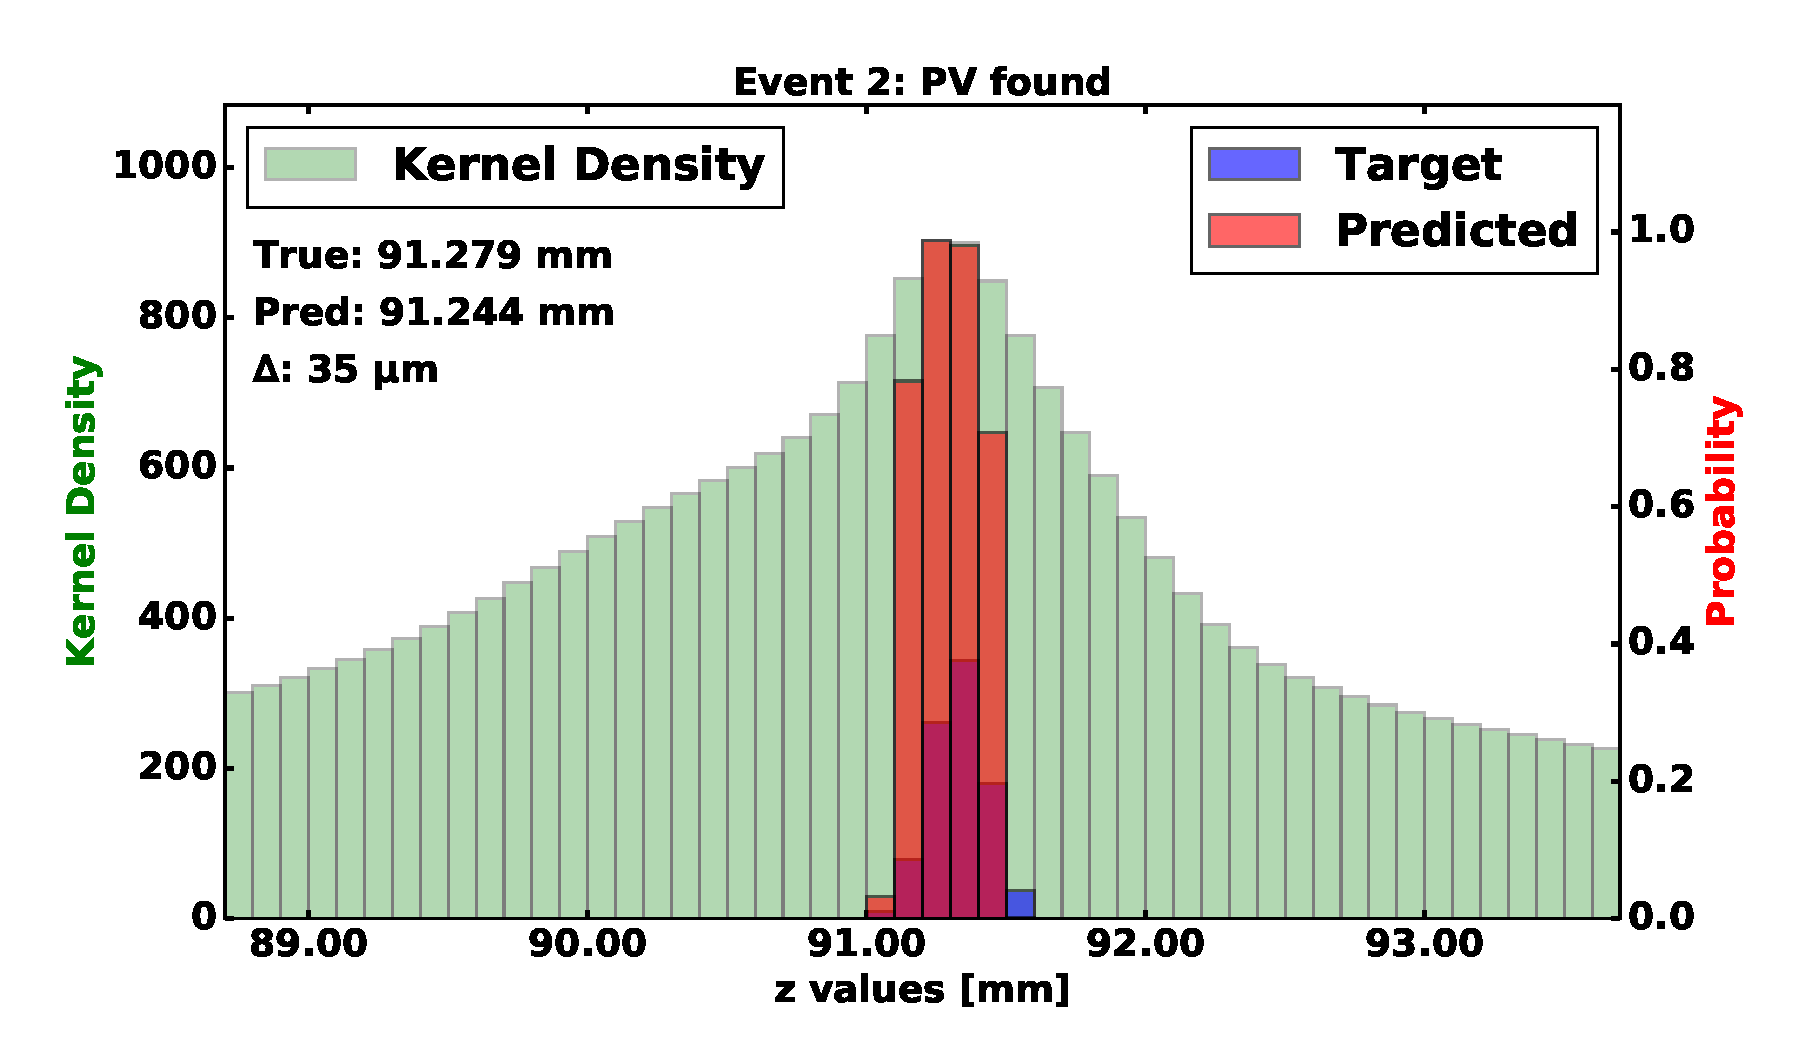
\includegraphics[width=1\textwidth, height=0.45\textwidth,trim=18 0 18 0]{images/120000_3layer_13.pdf}

        \end{center}
    \column{.5\textwidth}
        \begin{center}
           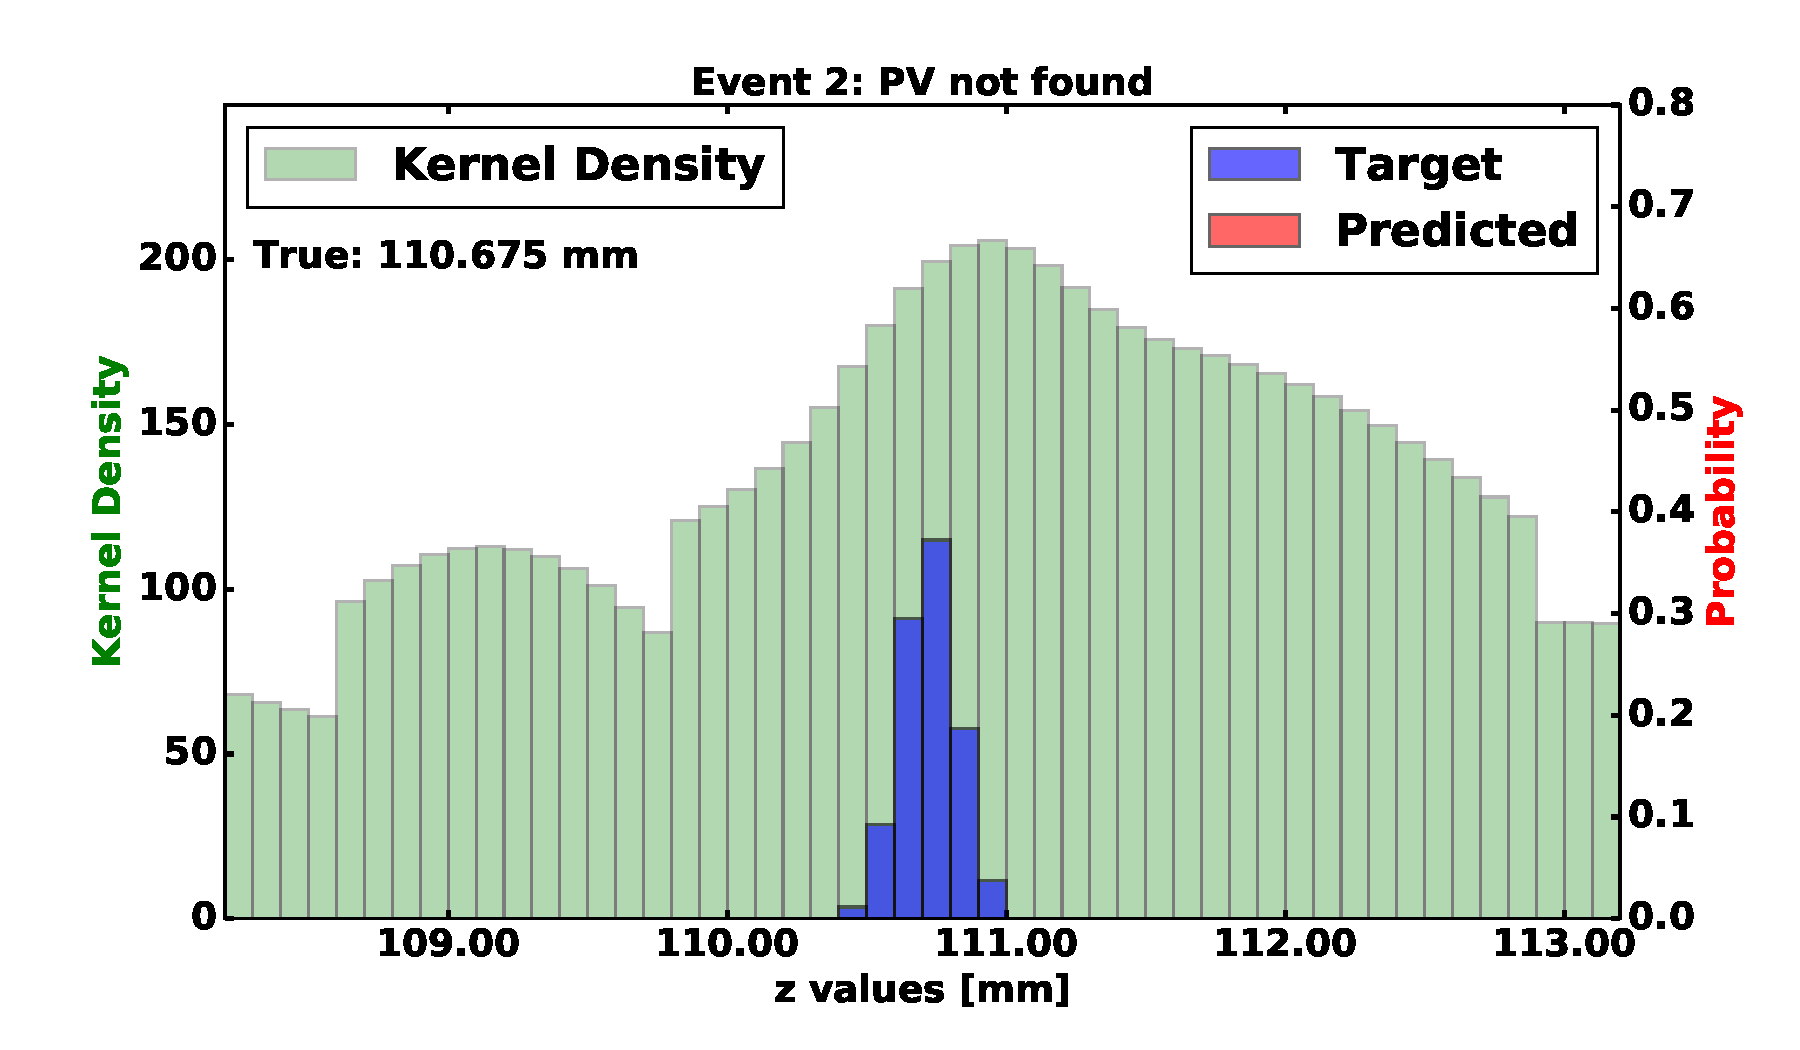
\includegraphics[width=1\textwidth, height=0.45\textwidth, trim=18 0 18 0]{images/120000_3layer_14.pdf}
    
           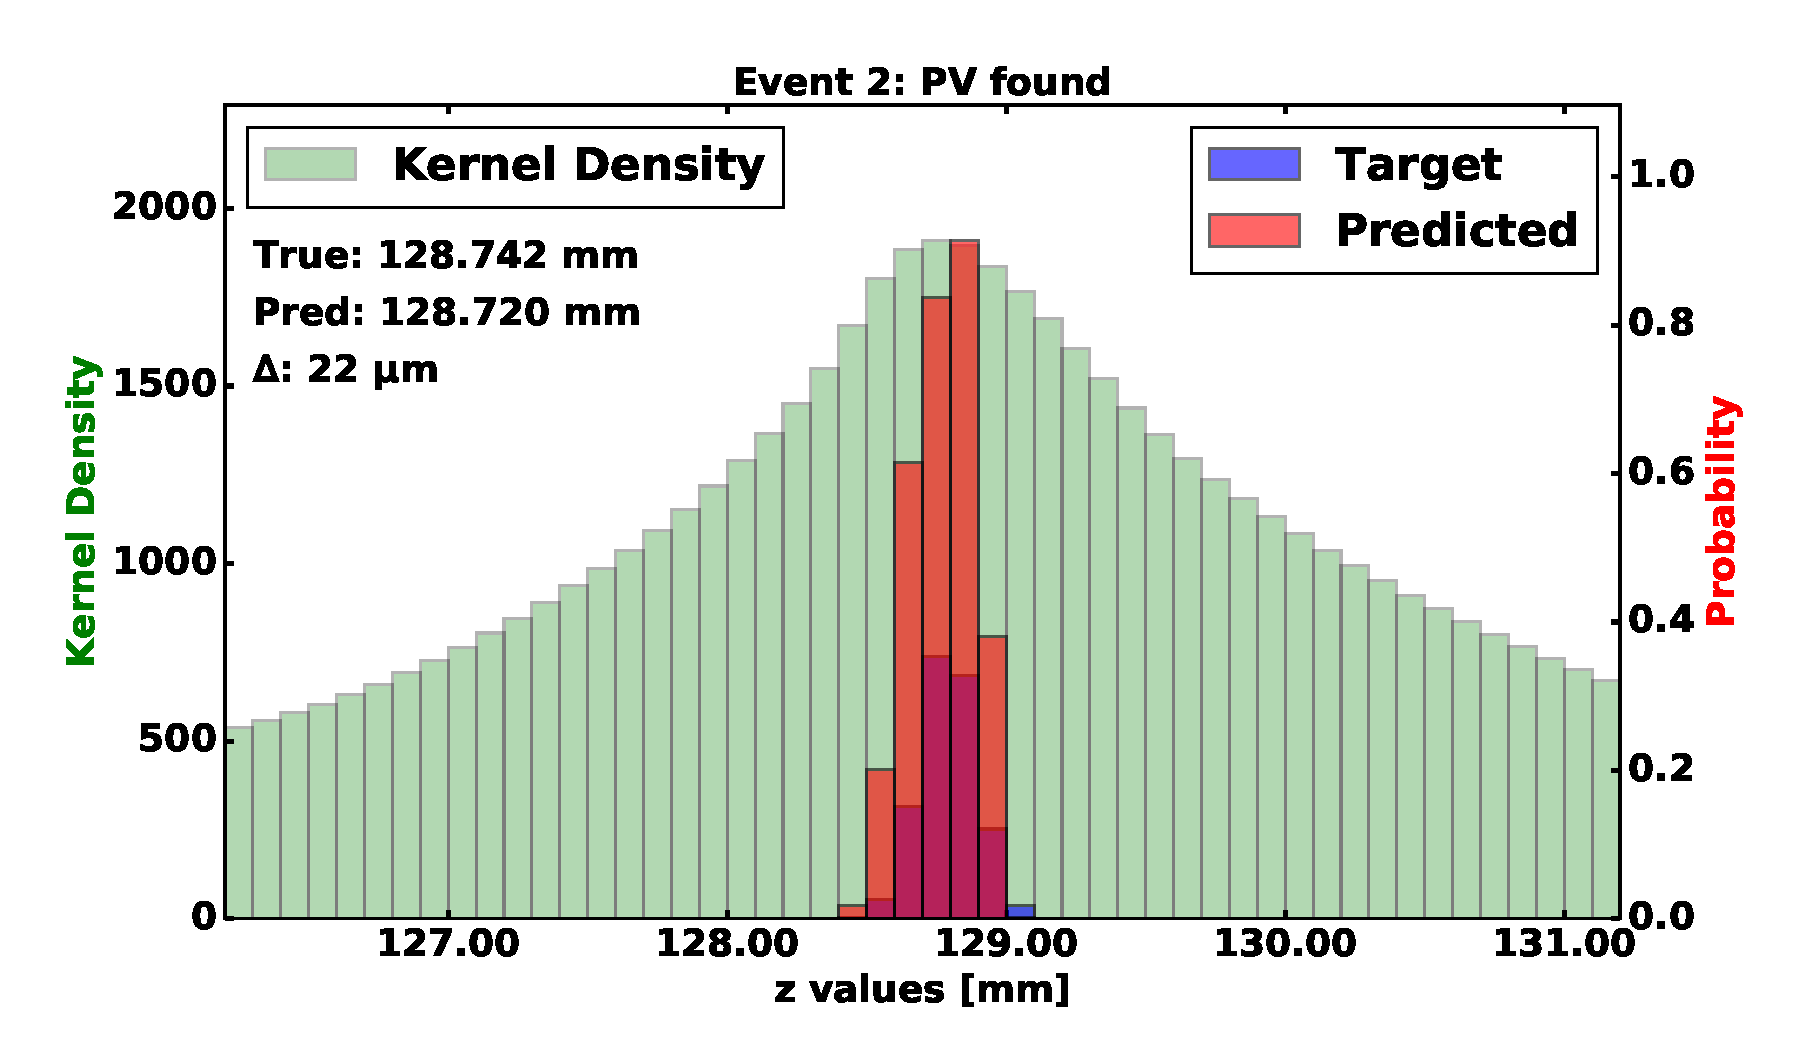
\includegraphics[width=1\textwidth, height=0.45\textwidth, trim=18 0 18 0]{images/120000_3layer_15.pdf}
       \end{center}
  \end{columns}
\end{frame}







% Part 7: RUI
\subsection{Quantitative Results }
\begin{frame}{Efficiencies and False Positive Rates}
\begin{table}[]
\centering
\begin{tabular}{cccc}
parameter & 2 CVN Layers &
3 CVN Layers & 4 CVN Layers \\ [0.3em]

$\epsilon \textrm{(Efficiency)}
 = \frac{\mbox{TP}}{\mbox{TP} + \mbox{FN}} $
&  $ \approx 58\% $  & $ \approx 70\% $ & $ \approx 75\% $ \\ [0.3em]
$ \textrm{False Positive rate}
 = \frac{\mbox{FP}}{\mbox{number of events}} $
 &  $\approx 0.07 $ & $\approx 0.08 $  & $ \approx 0.13 $ \\
 \end{tabular}
\end{table}
 \vskip -0.05in
  \begin{table}[]
      \centering
      \begin{tabular}{c|cc}
         & Found & Not found \\ \midrule
         Real PV & True positive & False negative\\
         Not a real PV & False positive & True negative
      \end{tabular}
  \end{table}
  \vskip -0.15in
  \begin{block}{True Positive}
    \begin{itemize}
    	\item search $ \pm 5 $ bins ($ \pm 500 \mu $m) around a real PV
    	\item at least 3 (4) bins with predicted probability
    	   $ > 1\% $ and 
    	   integrated probability $ > 20\%$.
    \end{itemize}

    \end{block}
    \begin{block}{False Positive}
    \begin{itemize}
        \item
           at least 3 (4) bins with individual probabilities $ > 1\% $ and
          integrated probability $ > 20\%$.
        \item 
        no real PV within $ \pm 5 $ bins ($ \pm 500 \mu $m) of that cluster.
    \end{itemize}
  \end{block}
\end{frame}





\section{Future Plans}
% Part 9
\subsection{Future plans}
\begin{frame}{Future plans}
    \begin{itemize}
        \item
          Model PV resolution as a function of the number of tracks; right now, the target
          function is always generated assuming $ \sigma_z = 100 \, \mu $m;
        \item
          Extract $ \sigma_z $ from predicted signals;
        \item
          Extend algorithm to find PV ($ x, \, y, \, z $) target functions,
          not just PV $ z $ target functions.
        \item
          Ask the algorithm (very nicely) to find Secondary Vertices as well;
          it should probably use both the original KDE histogram and the
          learned PV histogram as inputs.
          It may be possible to re-use some of the features generated by the
          convolutional layers.
        \item
          Integrate  KDE plus PV-finding code into an iterative tracking and vertexing
          algorithm; well-defined vertex positions may be able to serve as anchors for
          good tracks, restricting the roads to be searched.
        \item
          Optimize NN architecture to (i)~improve learning, (ii)~improve learning speed,
          (iii)~minimize inference costs (cycles and memory).
          Increase training sample.
    \end{itemize}
\end{frame}

\subsection{Questions}
\begin{frame}{Questions for ATLAS and CMS}
    \begin{itemize}
      \item
          Beam width ($x$, $y$): $\unit[40]{\mu m}$ for LHCb; what are the widths for ATLAS and CMS?
      \item
          Transverse resolution: $\unit[5\textup{--}15]{\mu m}$ for LHCb depending on number of tracks; what is it for ATLAS and CMS?
      \item
          Longitudinal resolution: $\unit[40\textup{--}100]{\mu m}$ for LHCb depending on number of tracks; what is it for ATLAS and CMS?
      \item
          Cleaning up prototracks based on IP could simplify kernel
      \item
          Can prototracking be done in the ATLAS and CMS triggers?
    \end{itemize}
\end{frame}


\backupbegin
\section{Backup}
% \subsection{Backup slides}
% \begin{frame}{Backup slide}
% \end{frame}
%
% \begin{frame}{Code}
% 	Code and presentations (as CI artifacts) available at: \url{https://gitlab.cern.ch/hschrein/lhcb_presentation}
% \end{frame}


\begin{frame}{More Predictions with Targets (3 CVN layers)}
  \begin{columns}[c]
    \column{.5\textwidth}
        \begin{center}
            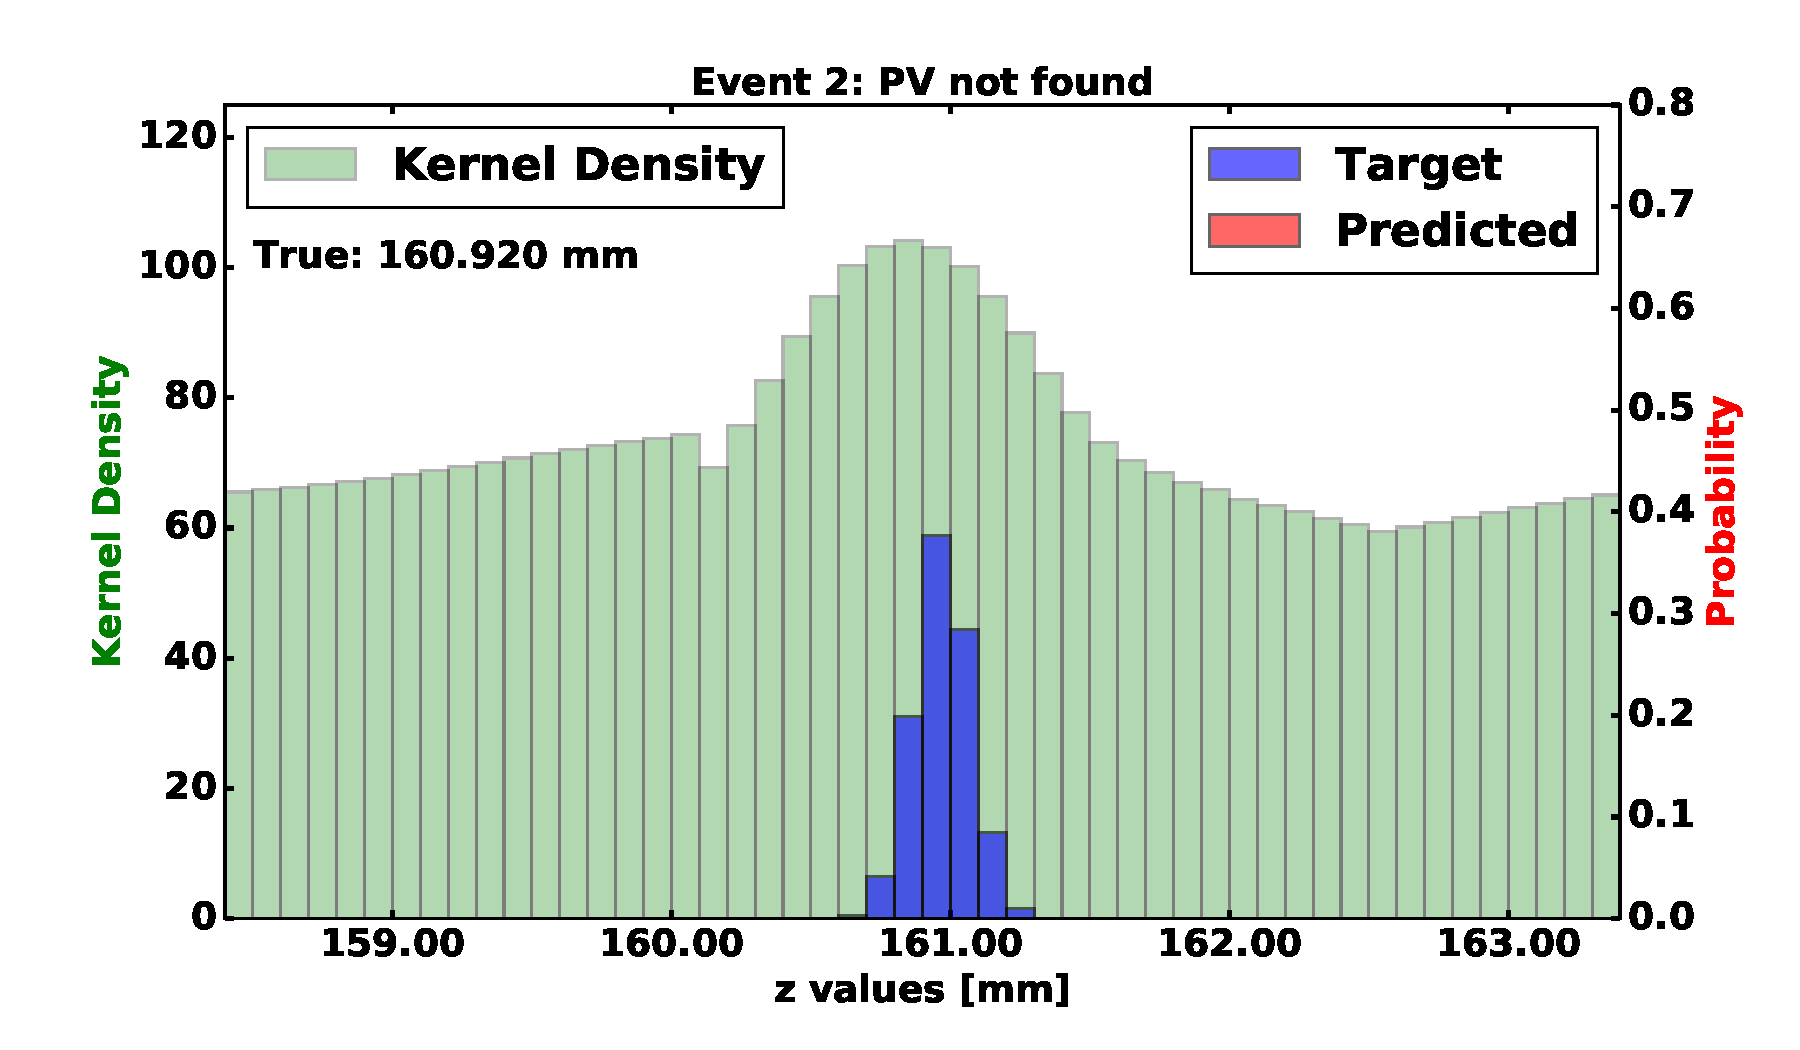
\includegraphics[width=1\textwidth,height=0.45\textwidth, trim=18 0 18 0]{images/120000_3layer_16.pdf}
    
            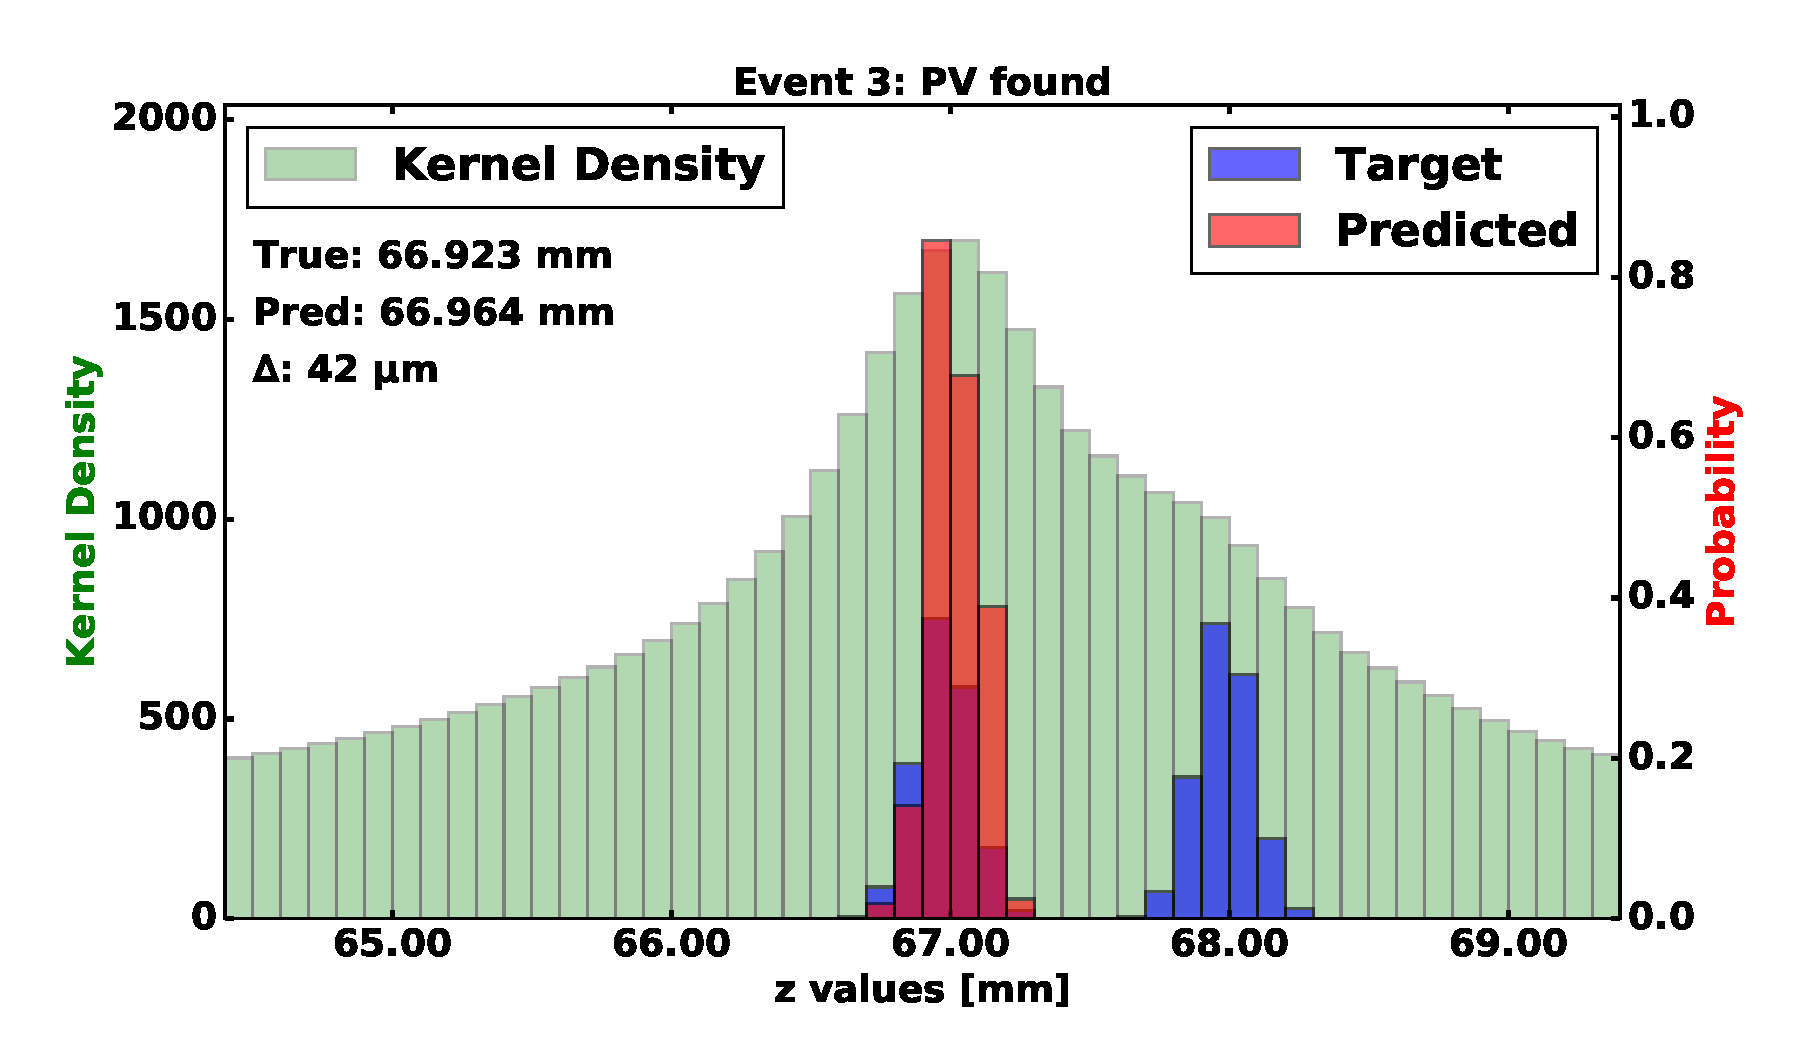
\includegraphics[width=1\textwidth, height=0.45\textwidth,trim=18 0 18 0]{images/120000_3layer_17.pdf}

        \end{center}
    \column{.5\textwidth}
        \begin{center}
           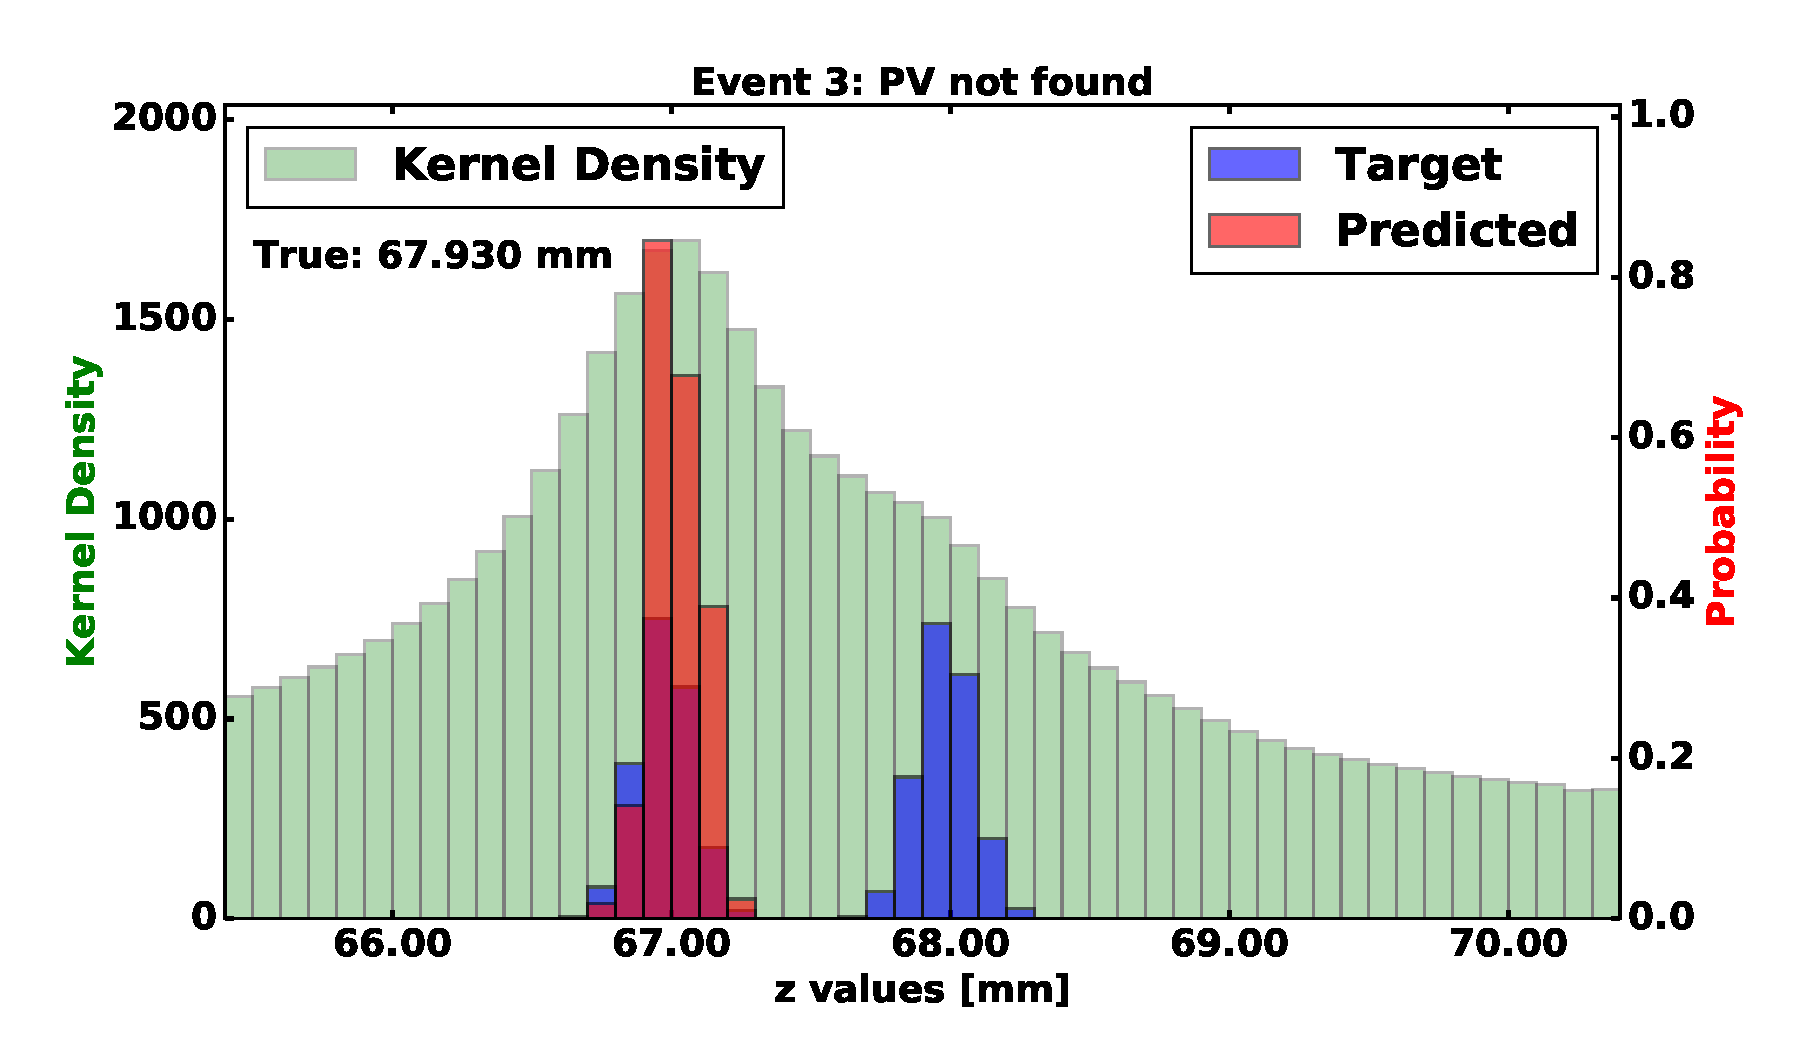
\includegraphics[width=1\textwidth, height=0.45\textwidth, trim=18 0 18 0]{images/120000_3layer_18.pdf}
    
           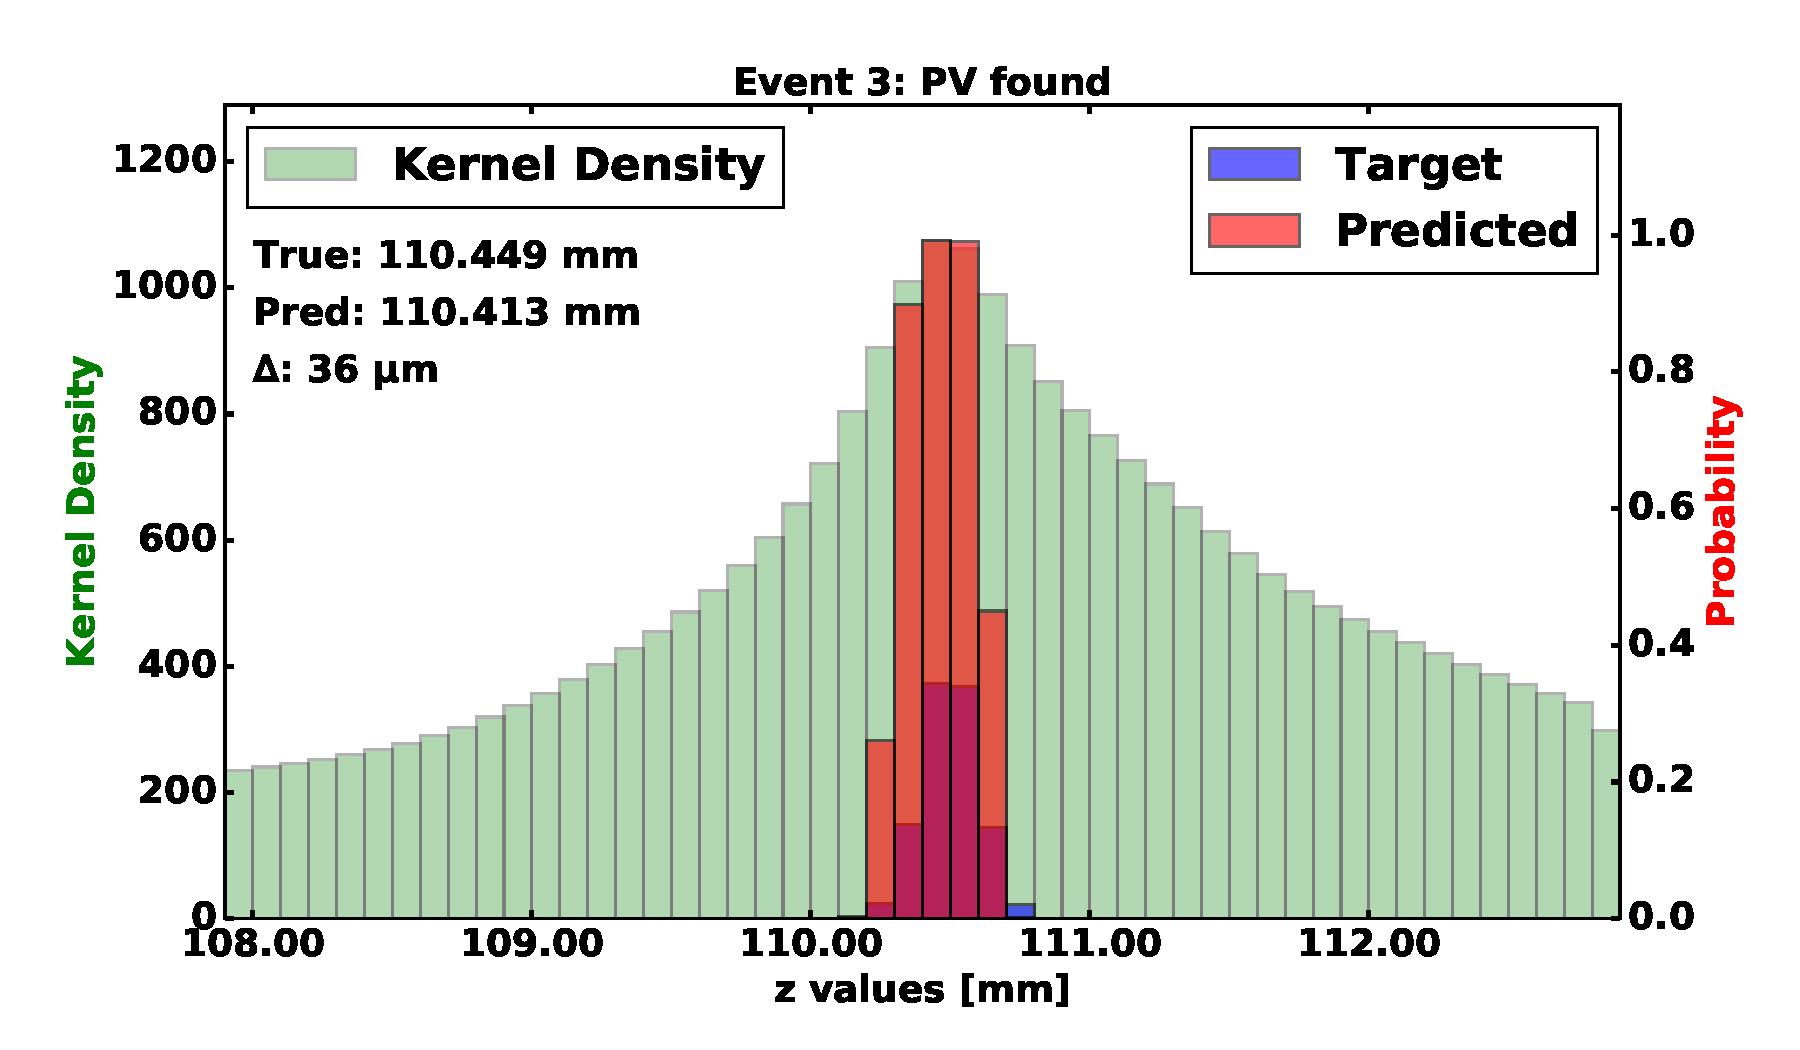
\includegraphics[width=1\textwidth, height=0.45\textwidth, trim=18 0 18 0]{images/120000_3layer_19.pdf}
       \end{center}
  \end{columns}
\end{frame}

\begin{frame}{More Predictions with Targets (3 CVN layers)}
  \begin{columns}[c]
    \column{.5\textwidth}
        \begin{center}
            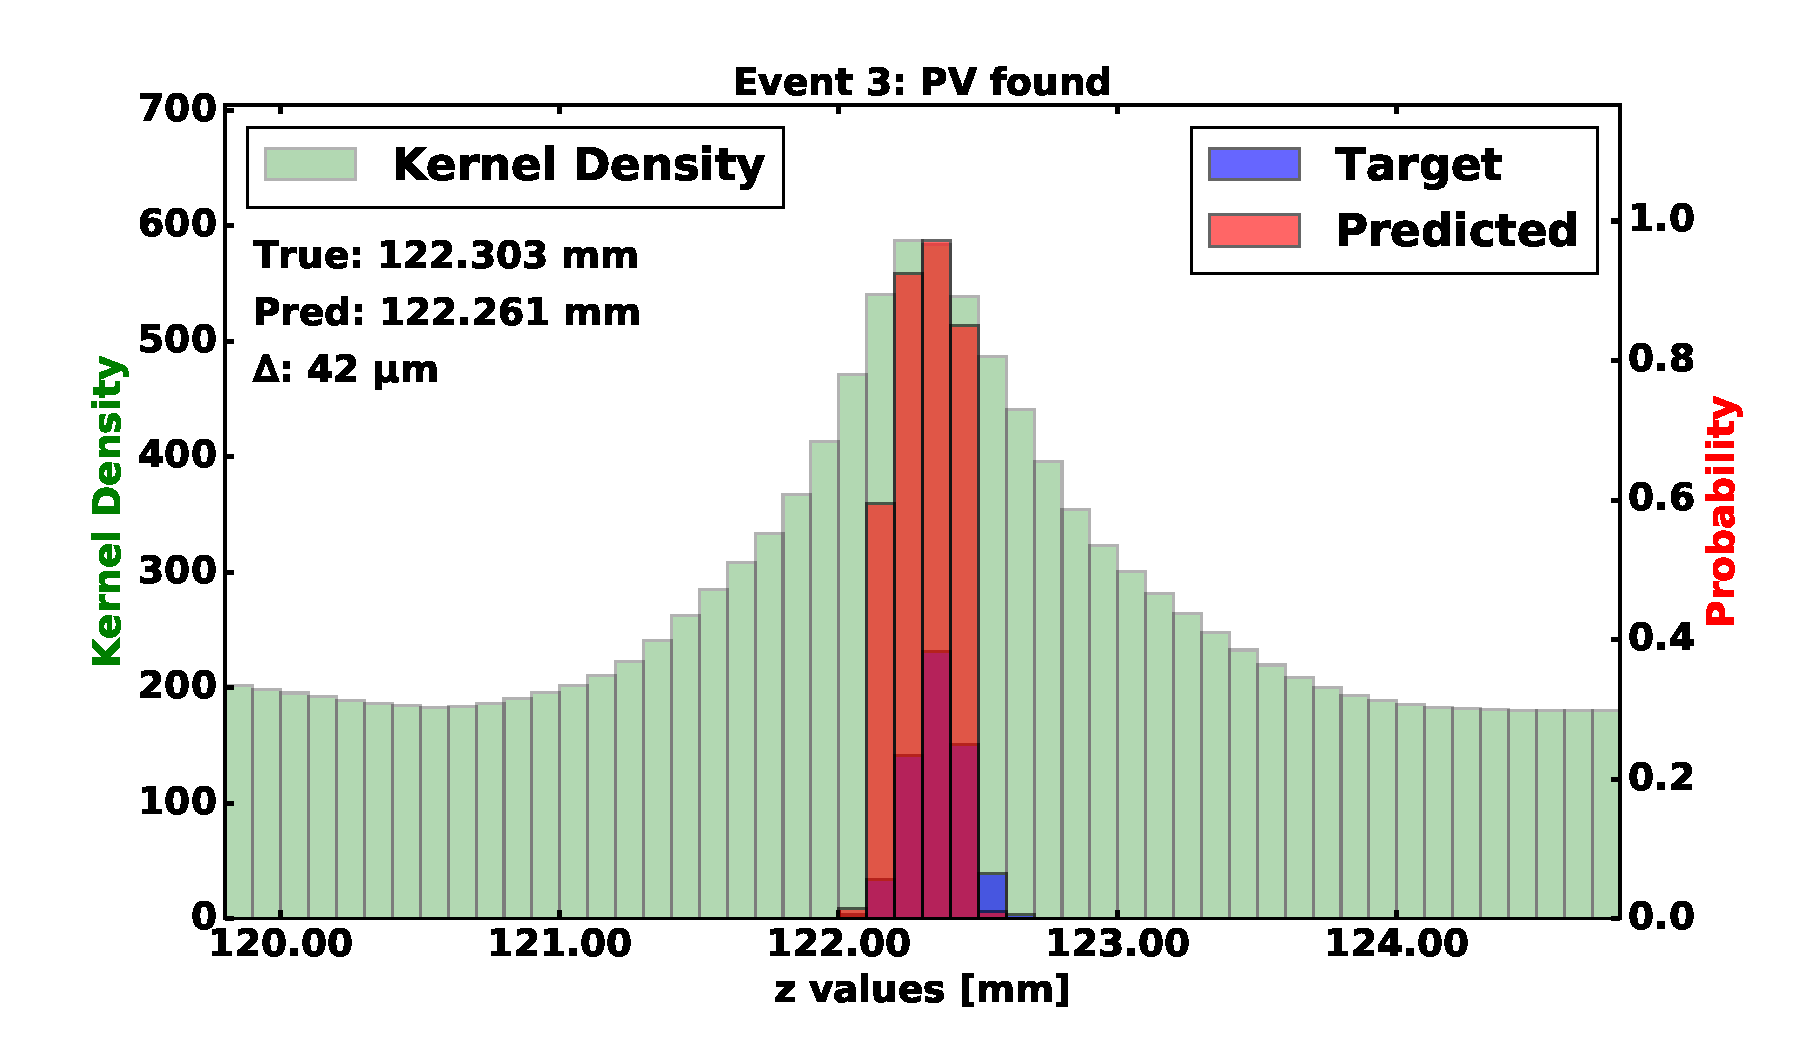
\includegraphics[width=1\textwidth,height=0.45\textwidth, trim=18 0 18 0]{images/120000_3layer_20.pdf}
    
            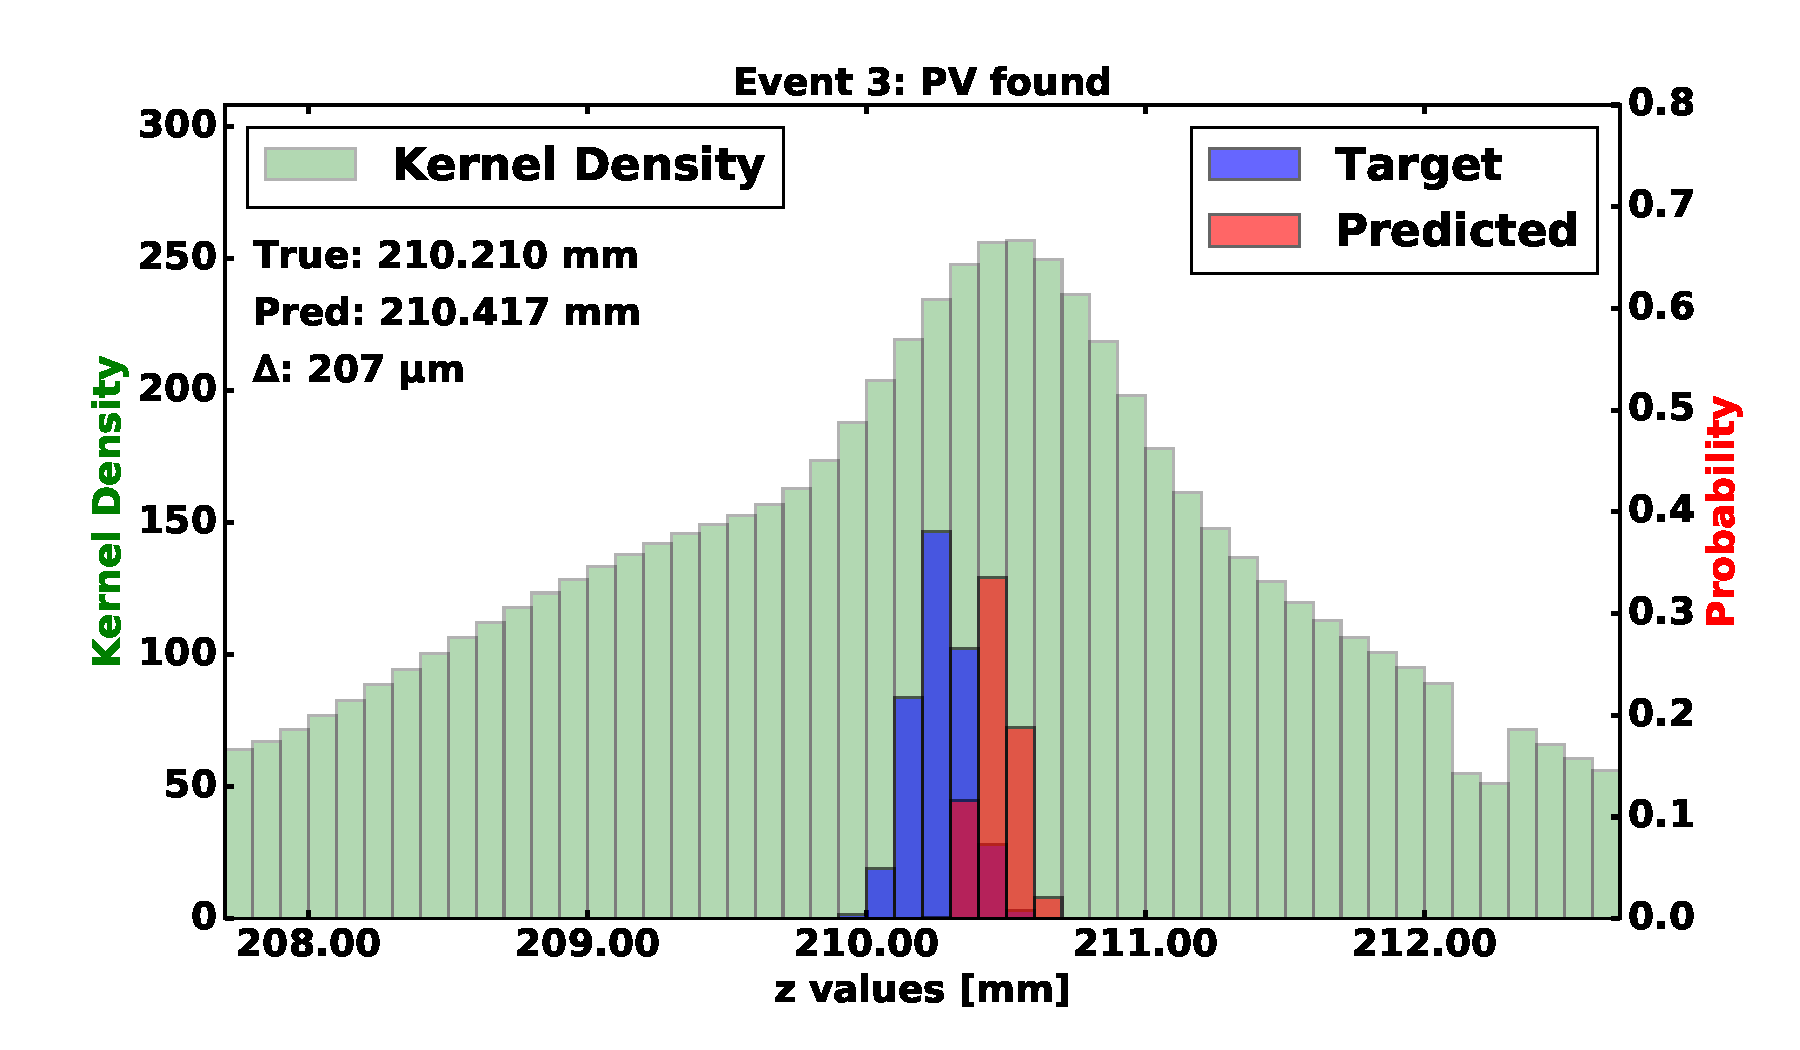
\includegraphics[width=1\textwidth, height=0.45\textwidth,trim=18 0 18 0]{images/120000_3layer_21.pdf}

        \end{center}
    \column{.5\textwidth}
        \begin{center}
           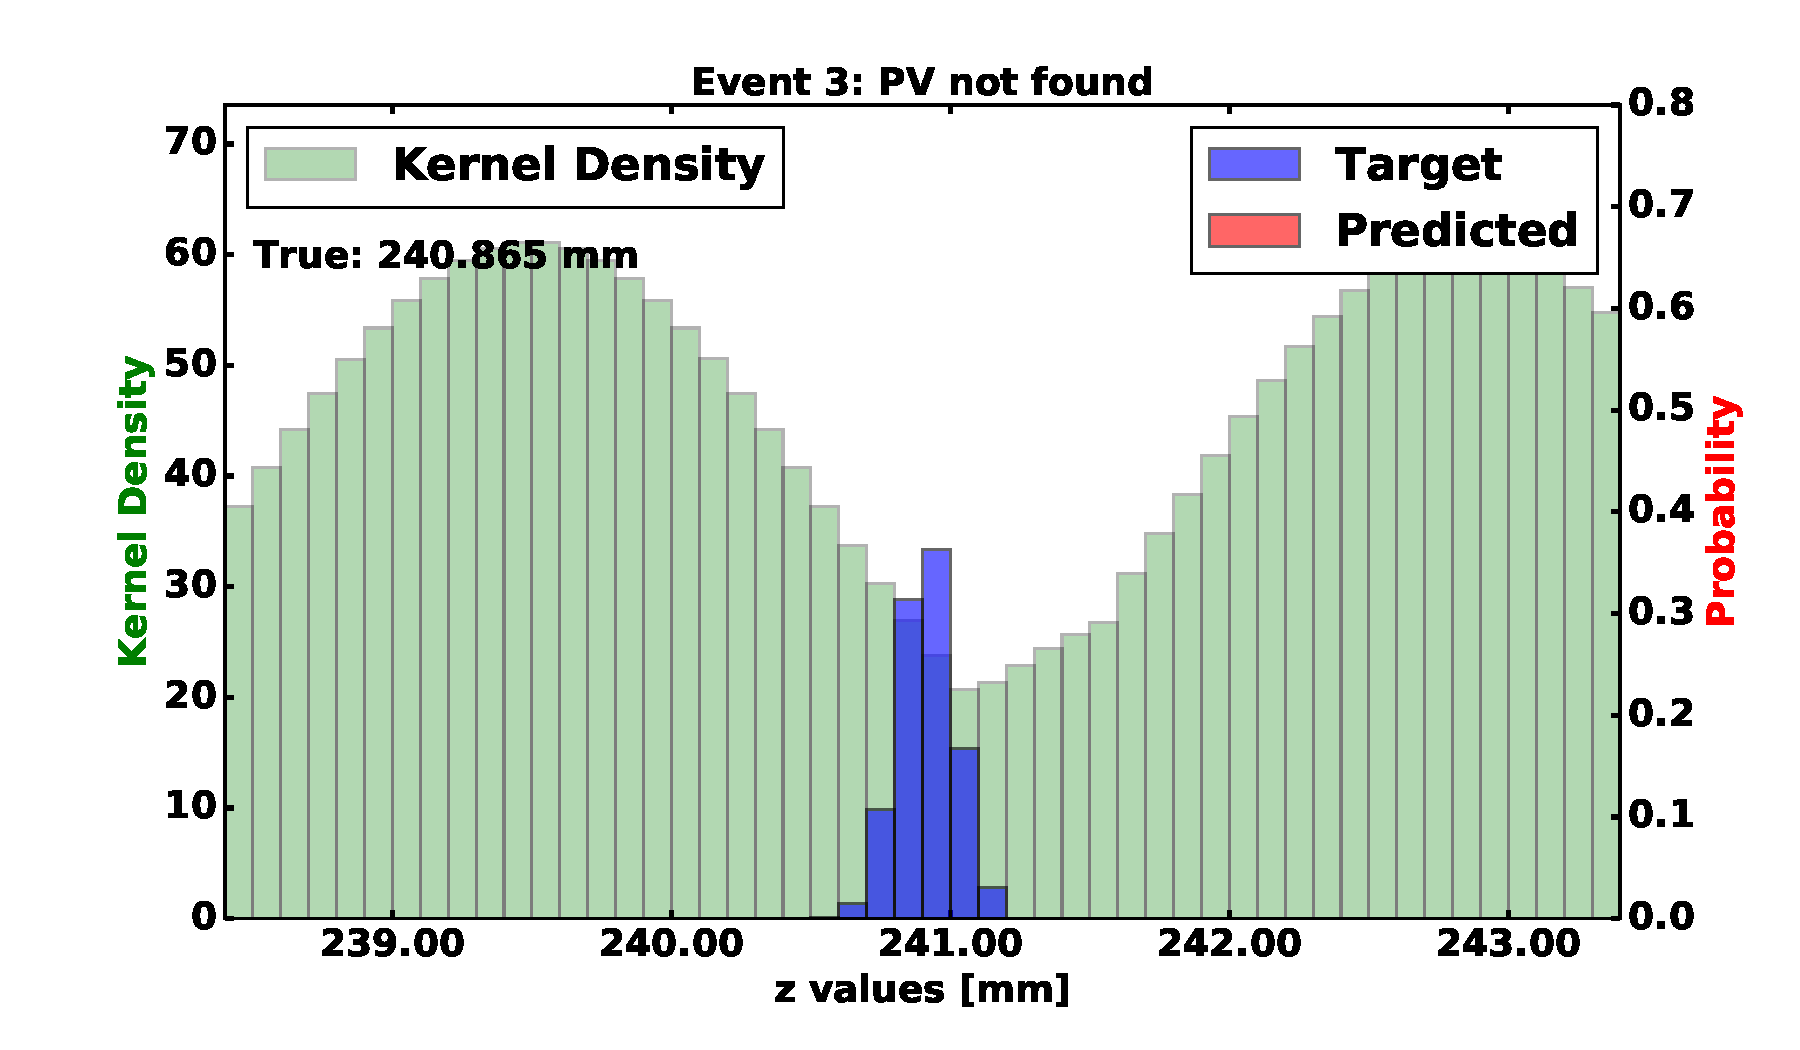
\includegraphics[width=1\textwidth, height=0.45\textwidth, trim=18 0 18 0]{images/120000_3layer_22.pdf}
    
           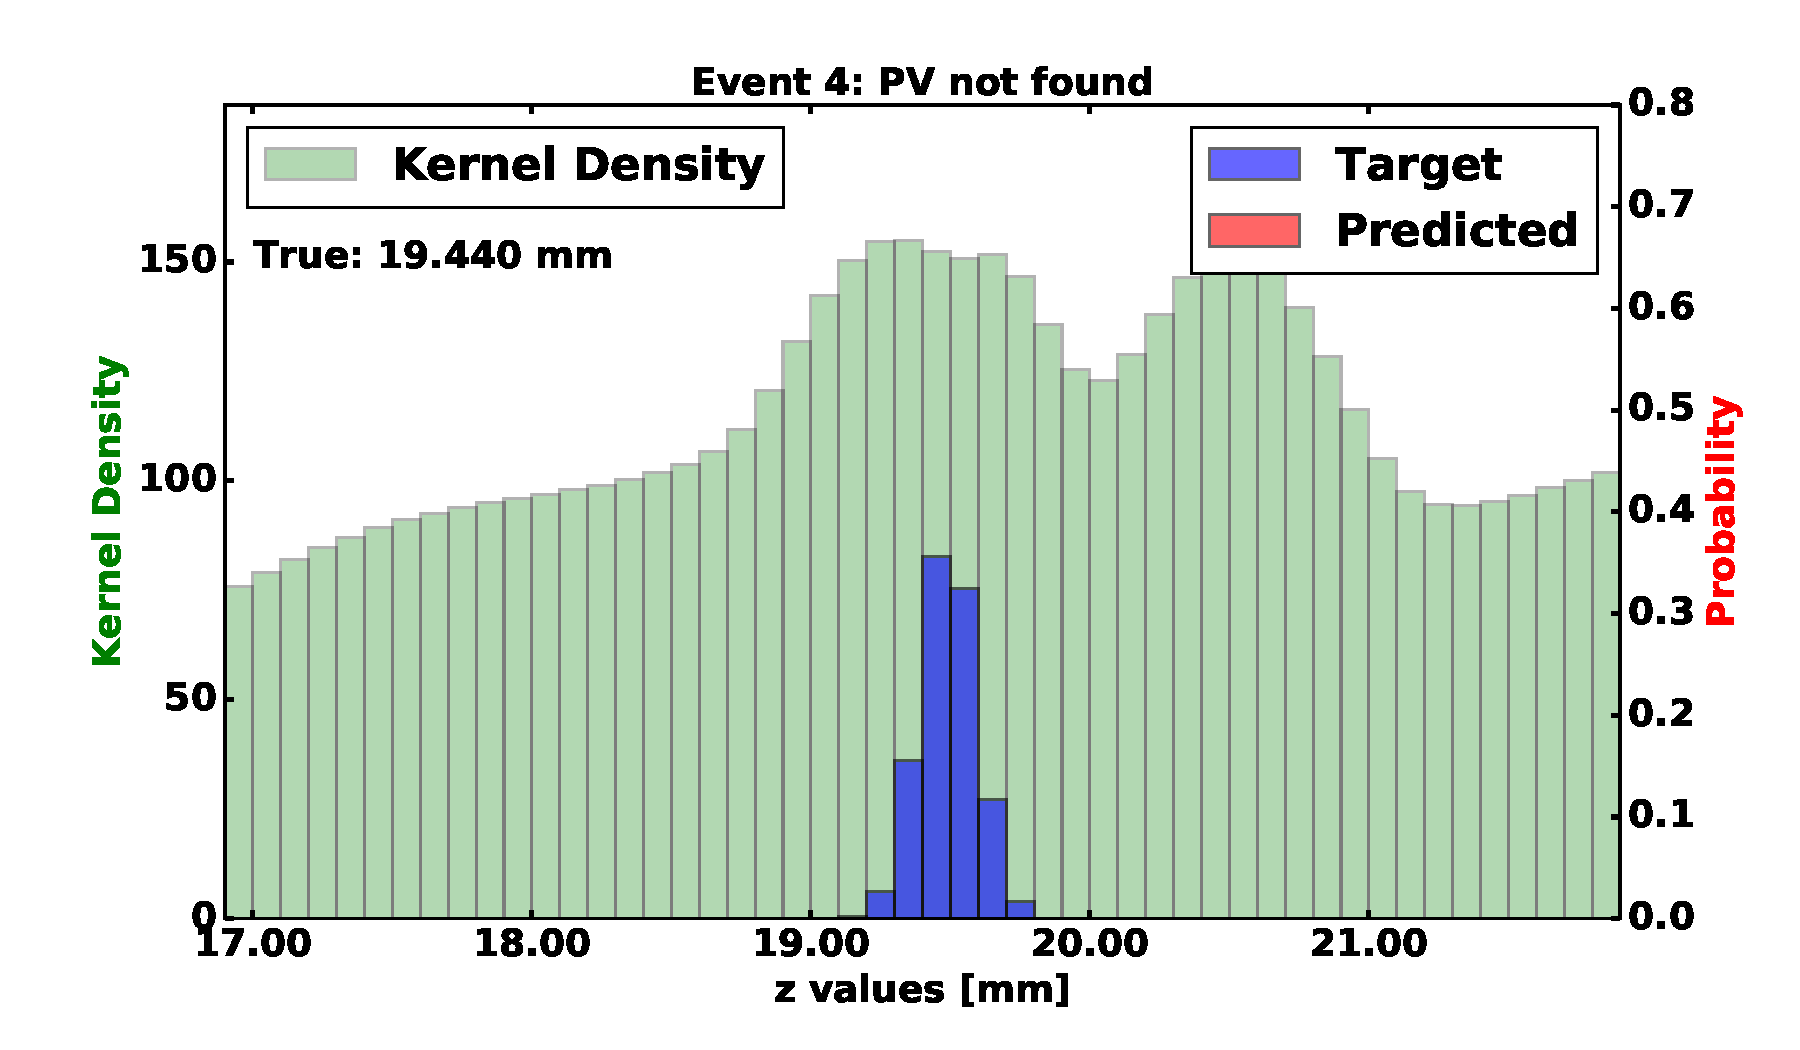
\includegraphics[width=1\textwidth, height=0.45\textwidth, trim=18 0 18 0]{images/120000_3layer_23.pdf}
       \end{center}
  \end{columns}
\end{frame}

\begin{frame}{More Predictions with Targets (3 CVN layers)}
  \begin{columns}[c]
    \column{.5\textwidth}
        \begin{center}
            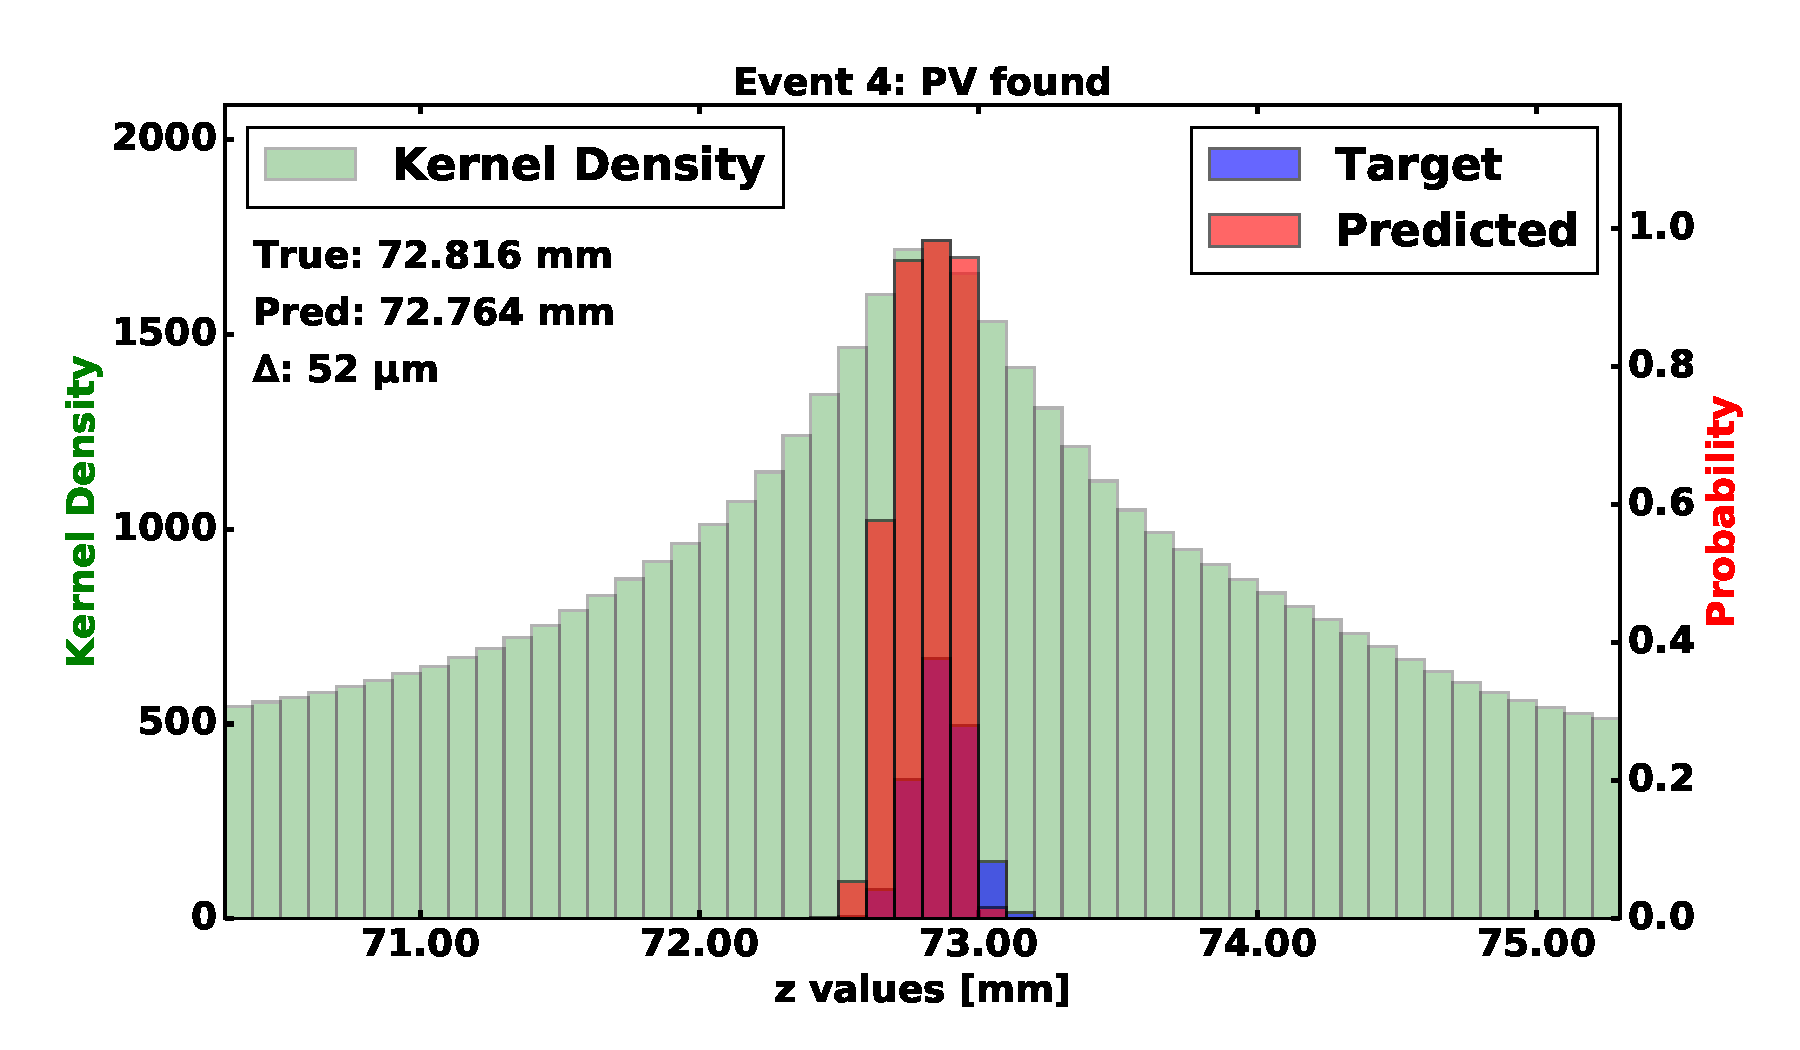
\includegraphics[width=1\textwidth,height=0.45\textwidth, trim=18 0 18 0]{images/120000_3layer_24.pdf}
    
            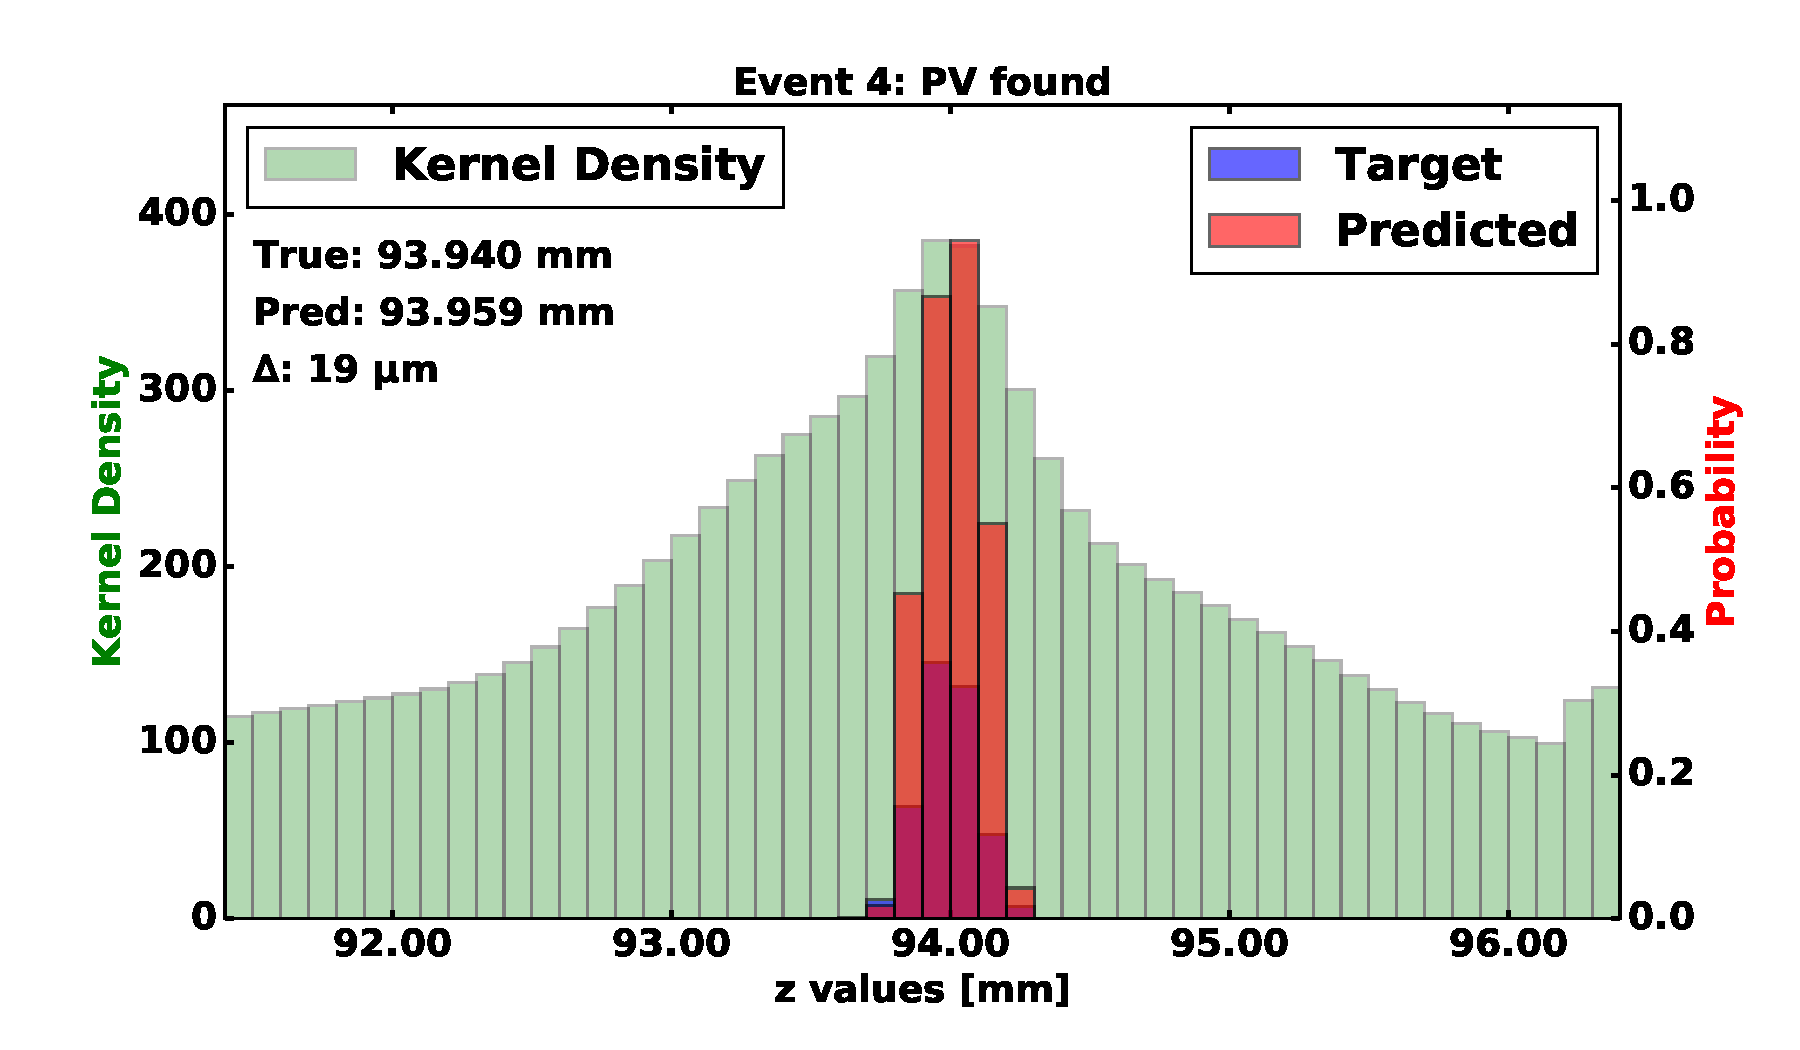
\includegraphics[width=1\textwidth, height=0.45\textwidth,trim=18 0 18 0]{images/120000_3layer_25.pdf}

        \end{center}
    \column{.5\textwidth}
        \begin{center}
           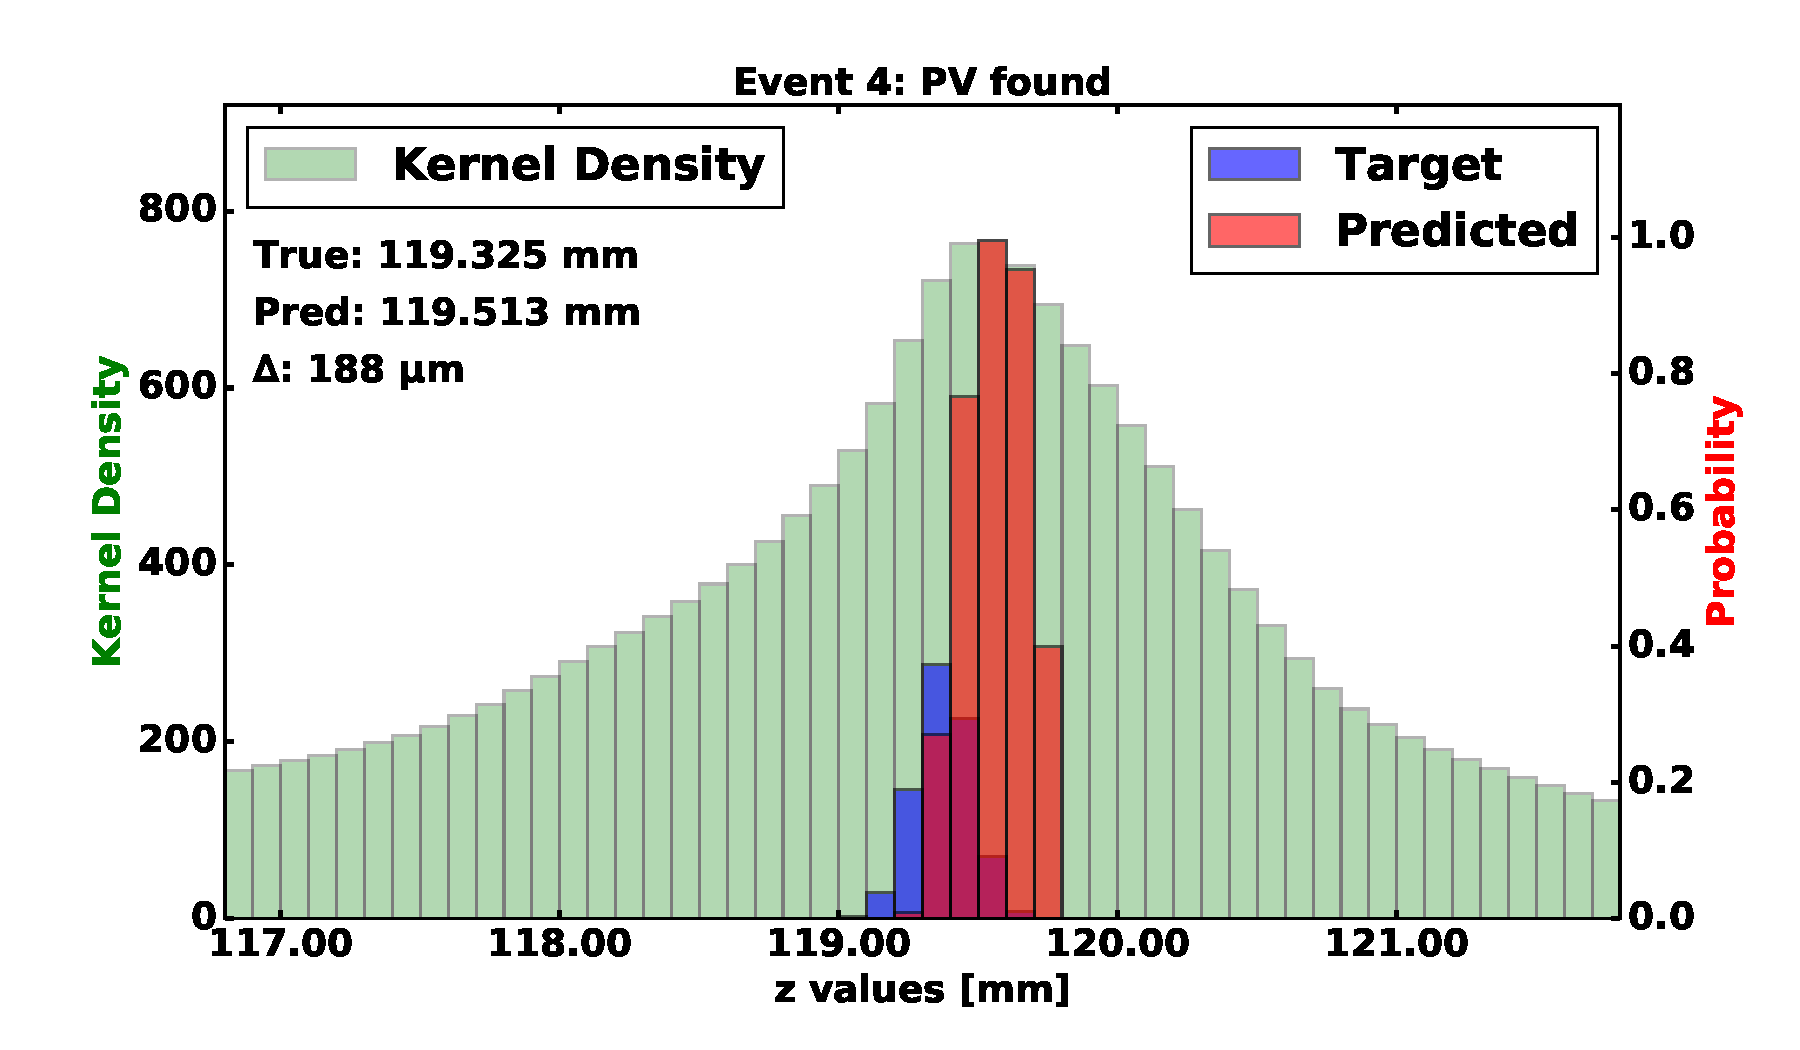
\includegraphics[width=1\textwidth, height=0.45\textwidth, trim=18 0 18 0]{images/120000_3layer_26.pdf}
    
           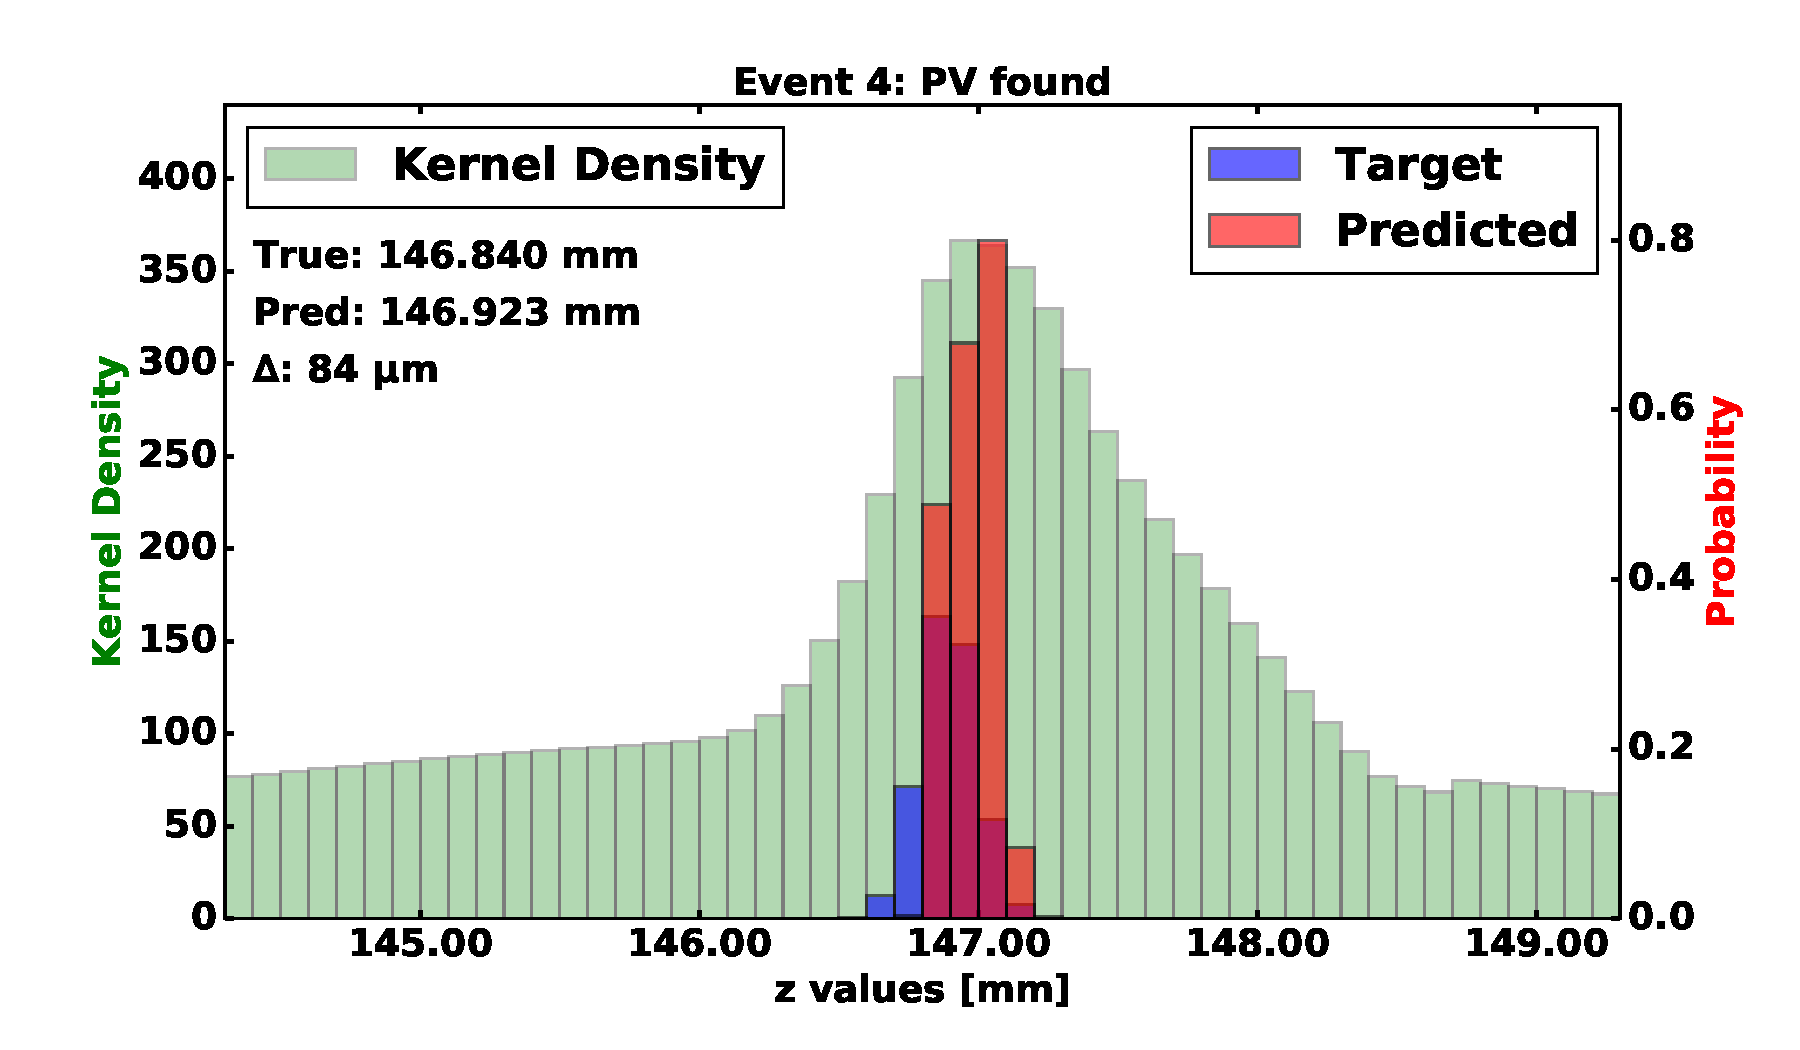
\includegraphics[width=1\textwidth, height=0.45\textwidth, trim=18 0 18 0]{images/120000_3layer_27.pdf}
       \end{center}
  \end{columns}
\end{frame}

\begin{frame}{More Predictions with Targets (3 CVN layers)}
  \begin{columns}[c]
    \column{.5\textwidth}
        \begin{center}
            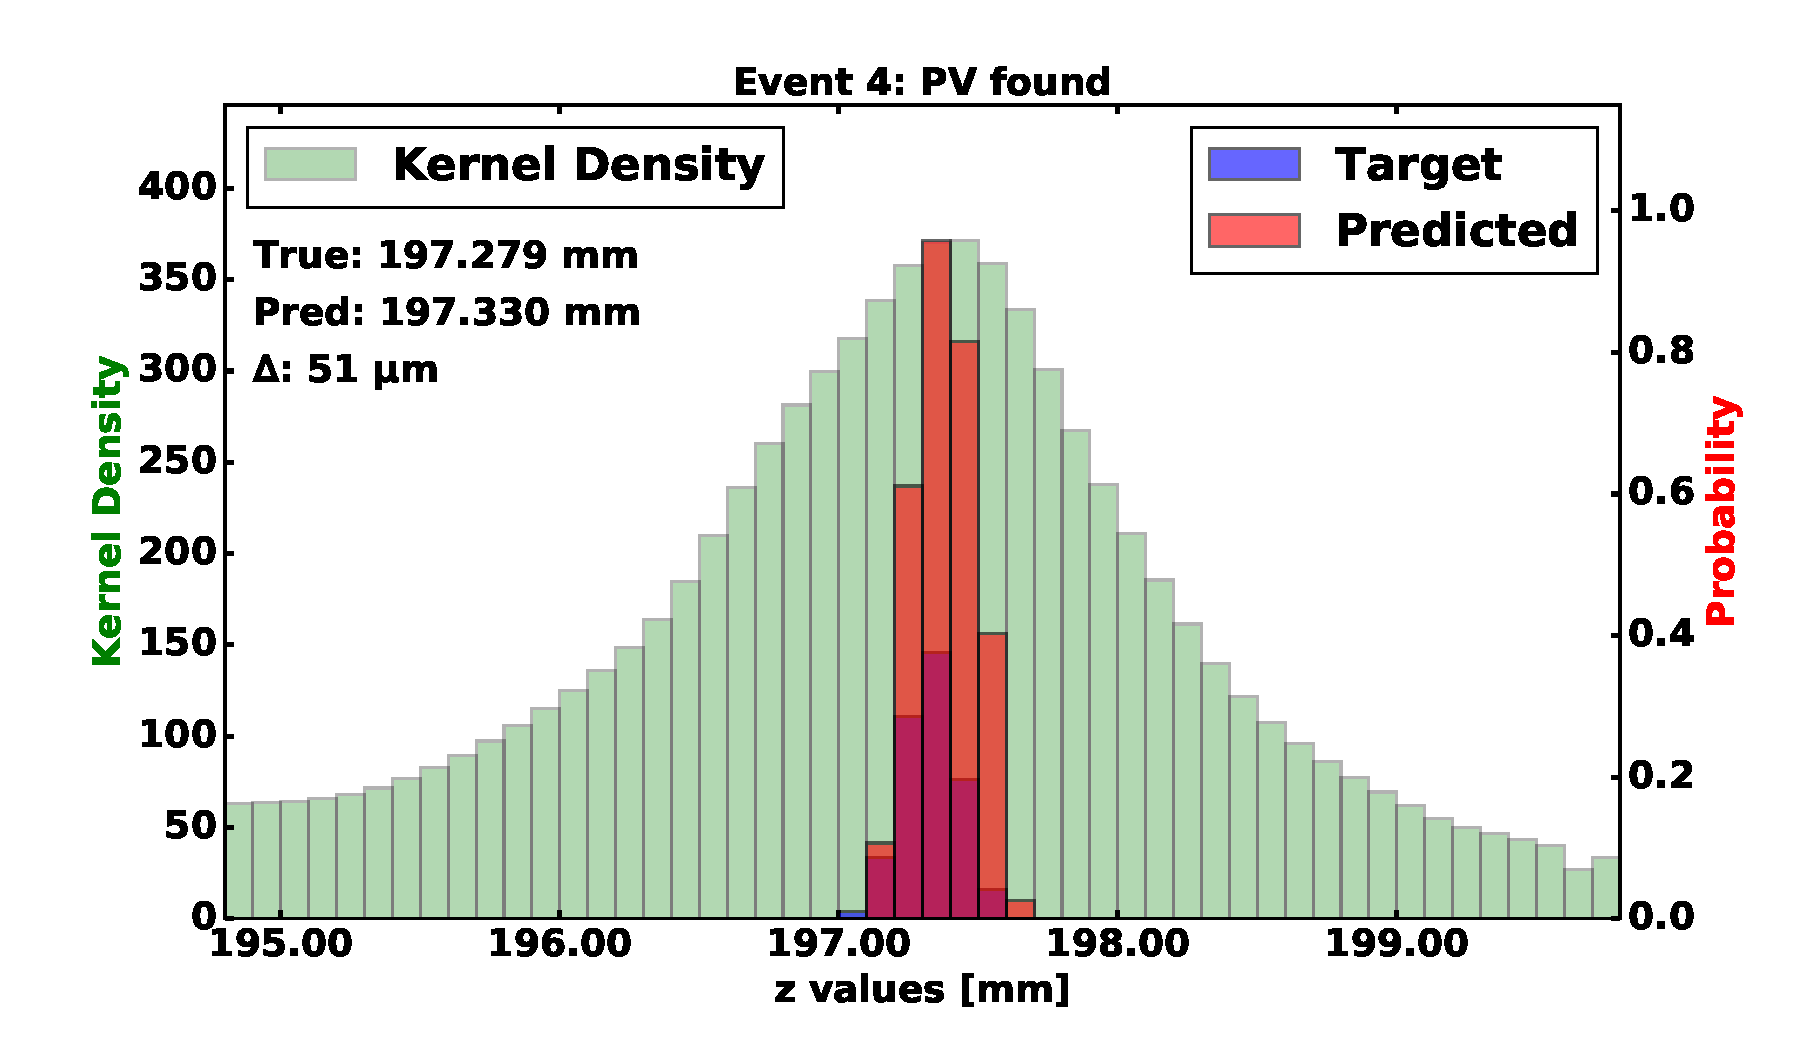
\includegraphics[width=1\textwidth,height=0.45\textwidth, trim=18 0 18 0]{images/120000_3layer_28.pdf}
    
            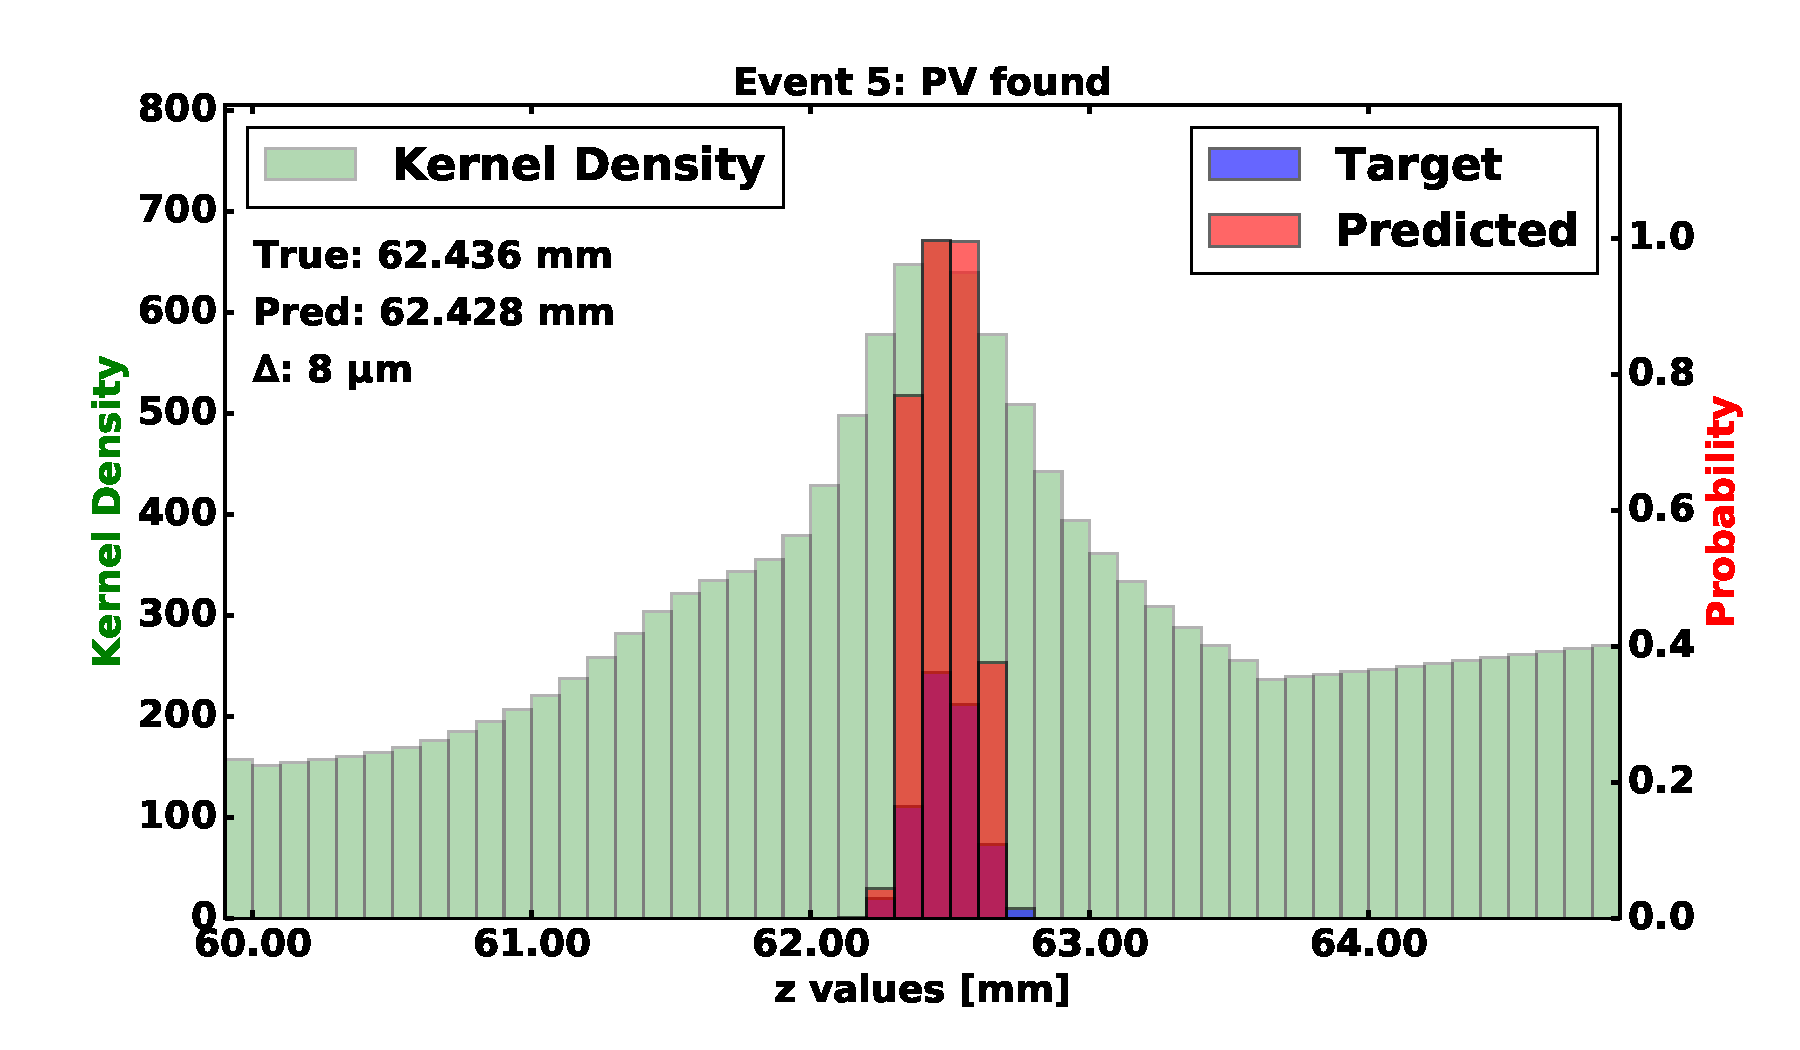
\includegraphics[width=1\textwidth, height=0.45\textwidth,trim=18 0 18 0]{images/120000_3layer_29.pdf}

        \end{center}
    \column{.5\textwidth}
        \begin{center}
           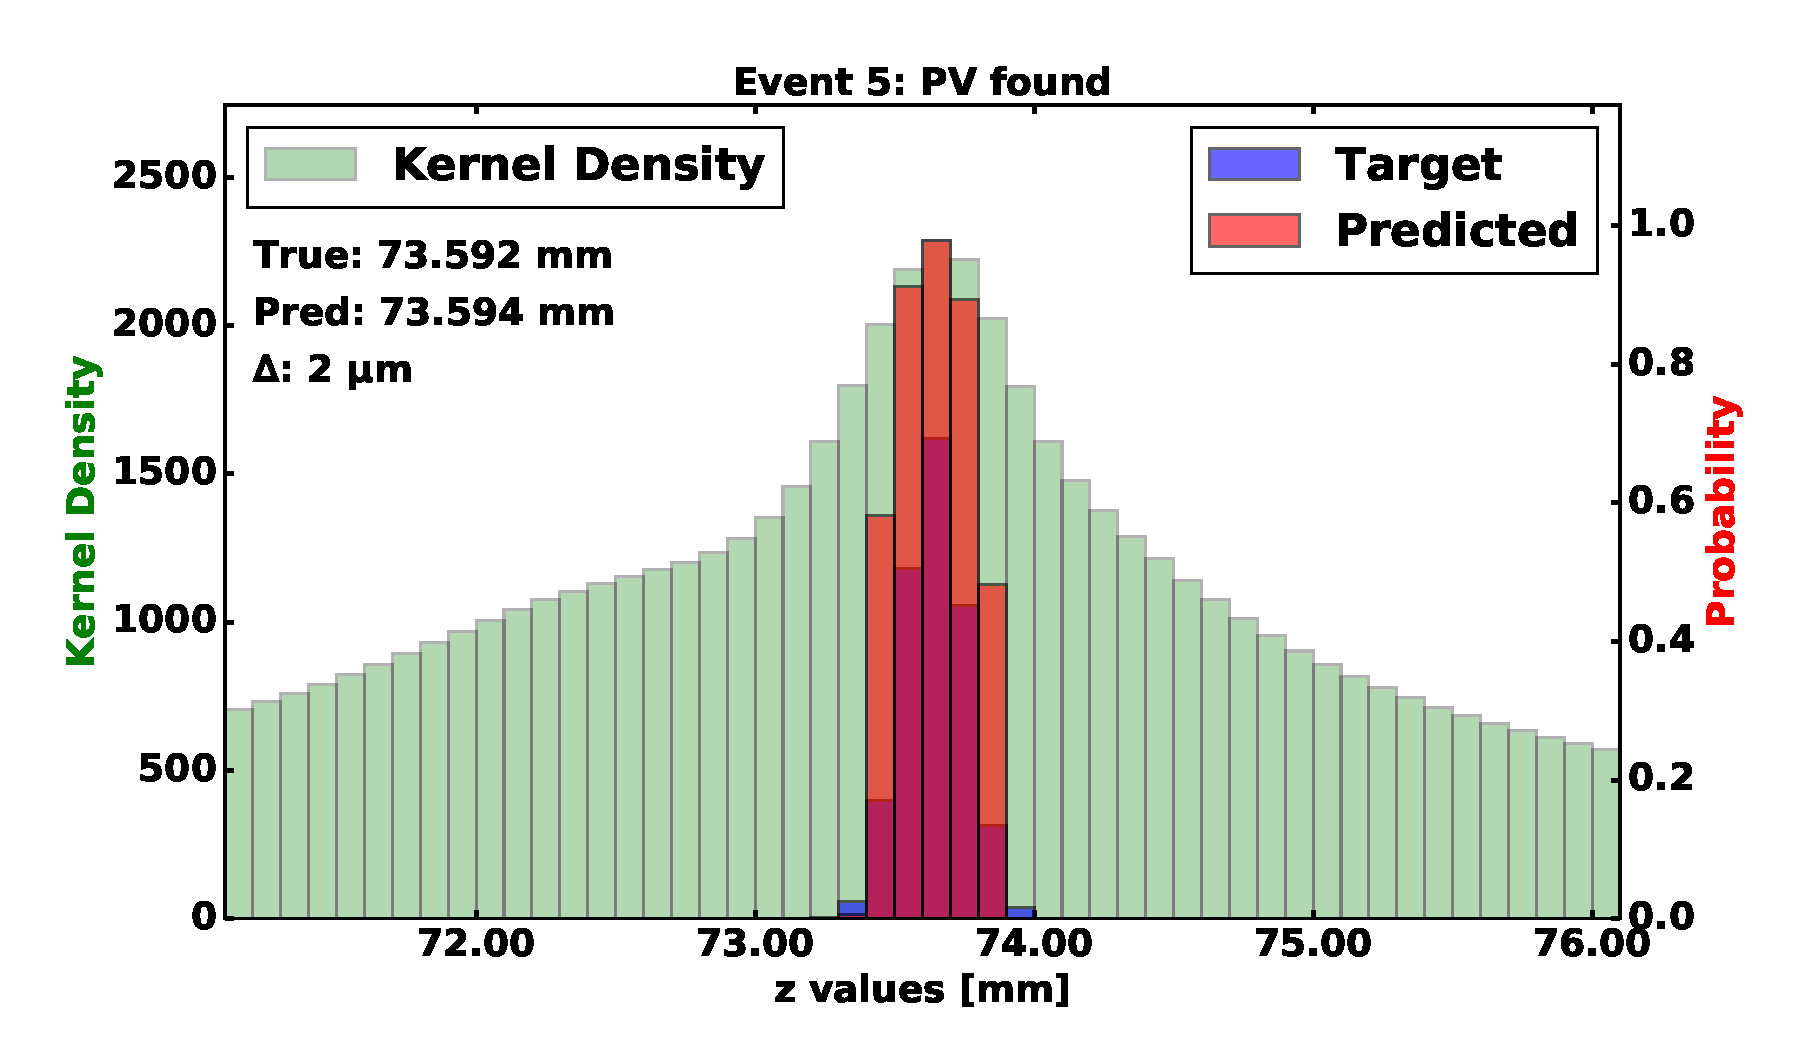
\includegraphics[width=1\textwidth, height=0.45\textwidth, trim=18 0 18 0]{images/120000_3layer_30.pdf}
    
           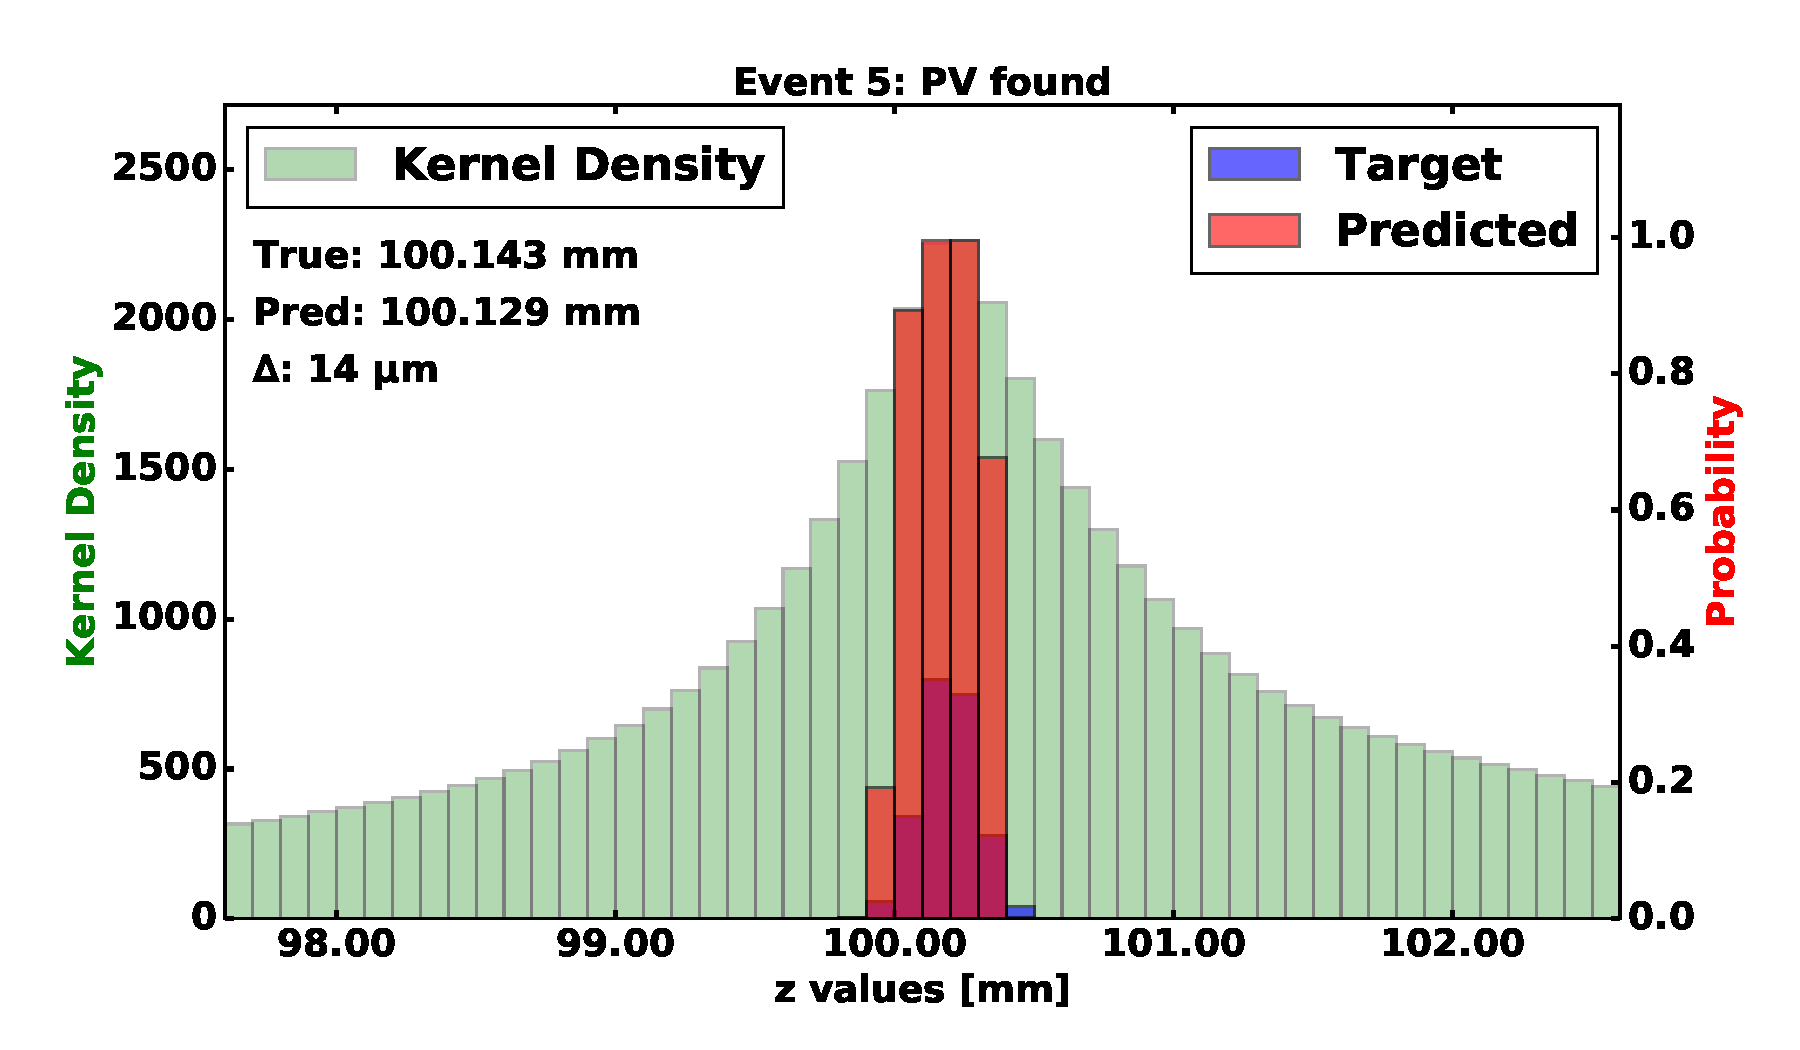
\includegraphics[width=1\textwidth, height=0.45\textwidth, trim=18 0 18 0]{images/120000_3layer_31.pdf}
       \end{center}
  \end{columns}
\end{frame}

\begin{frame}{More Predictions with Targets (3 CVN layers)}
  \begin{columns}[c]
    \column{.5\textwidth}
        \begin{center}
            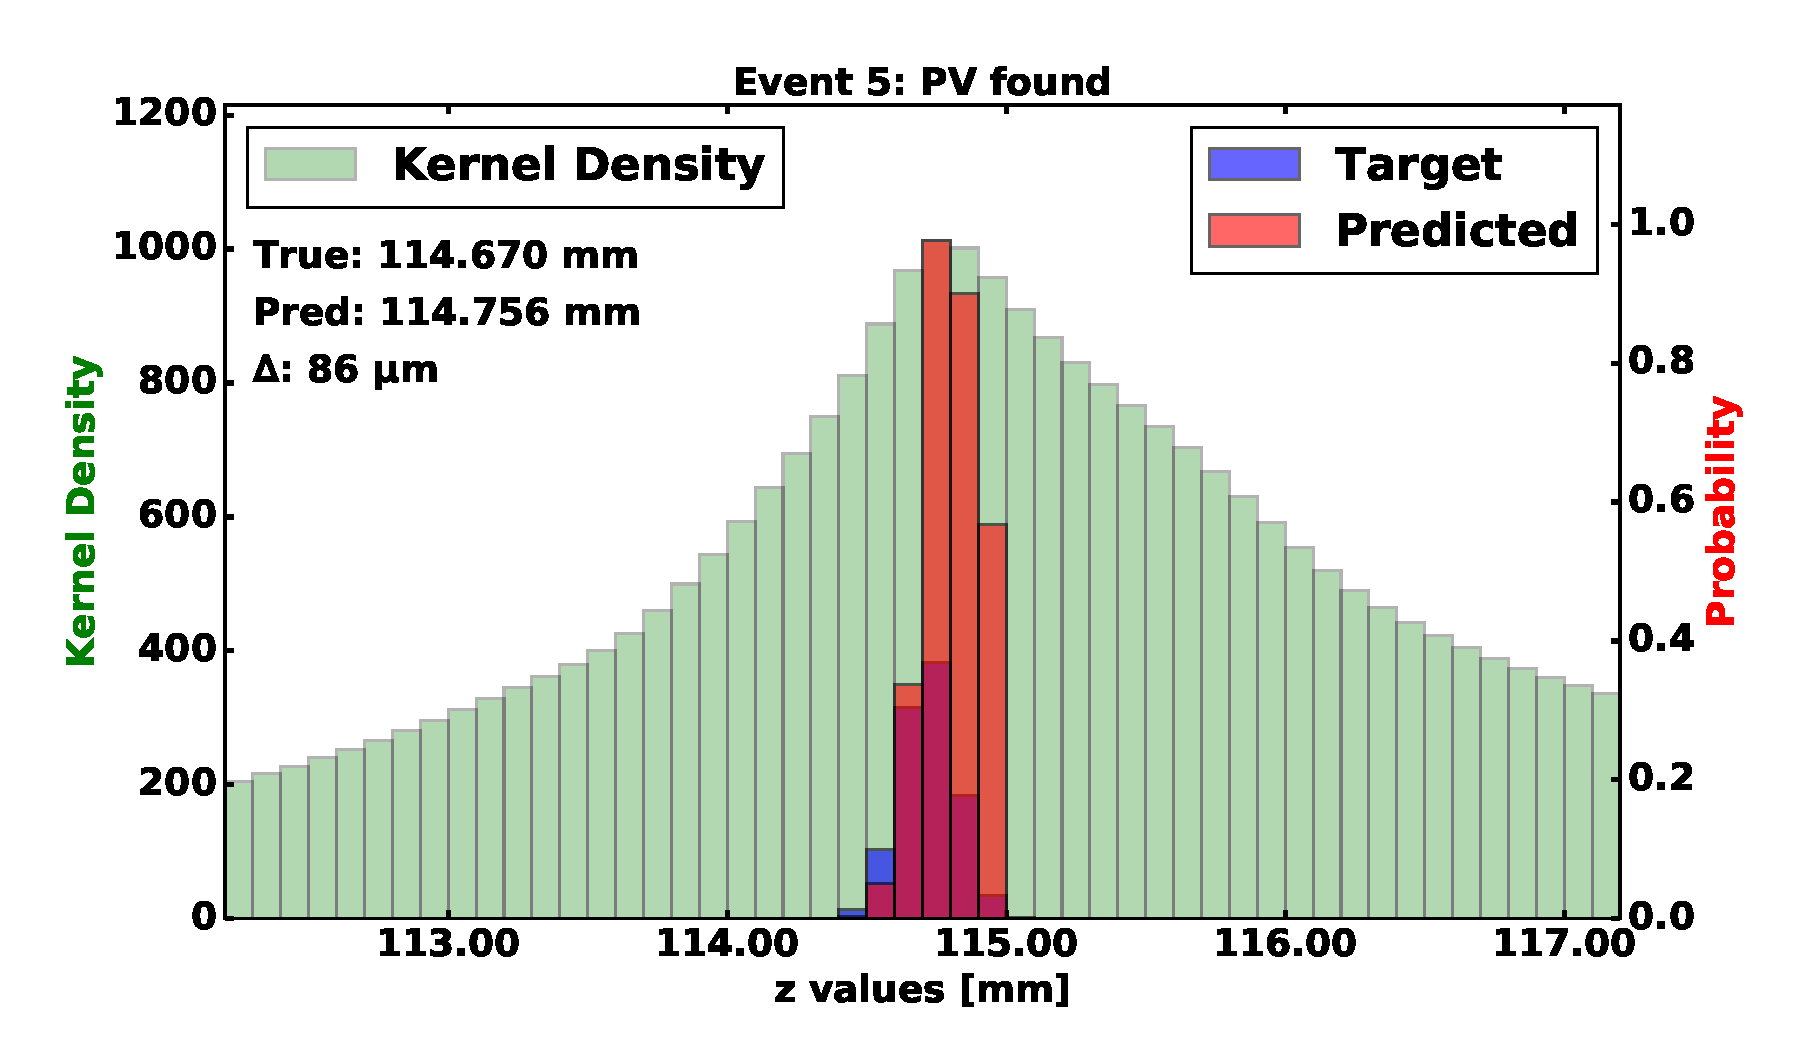
\includegraphics[width=1\textwidth,height=0.45\textwidth, trim=18 0 18 0]{images/120000_3layer_32.pdf}
    
            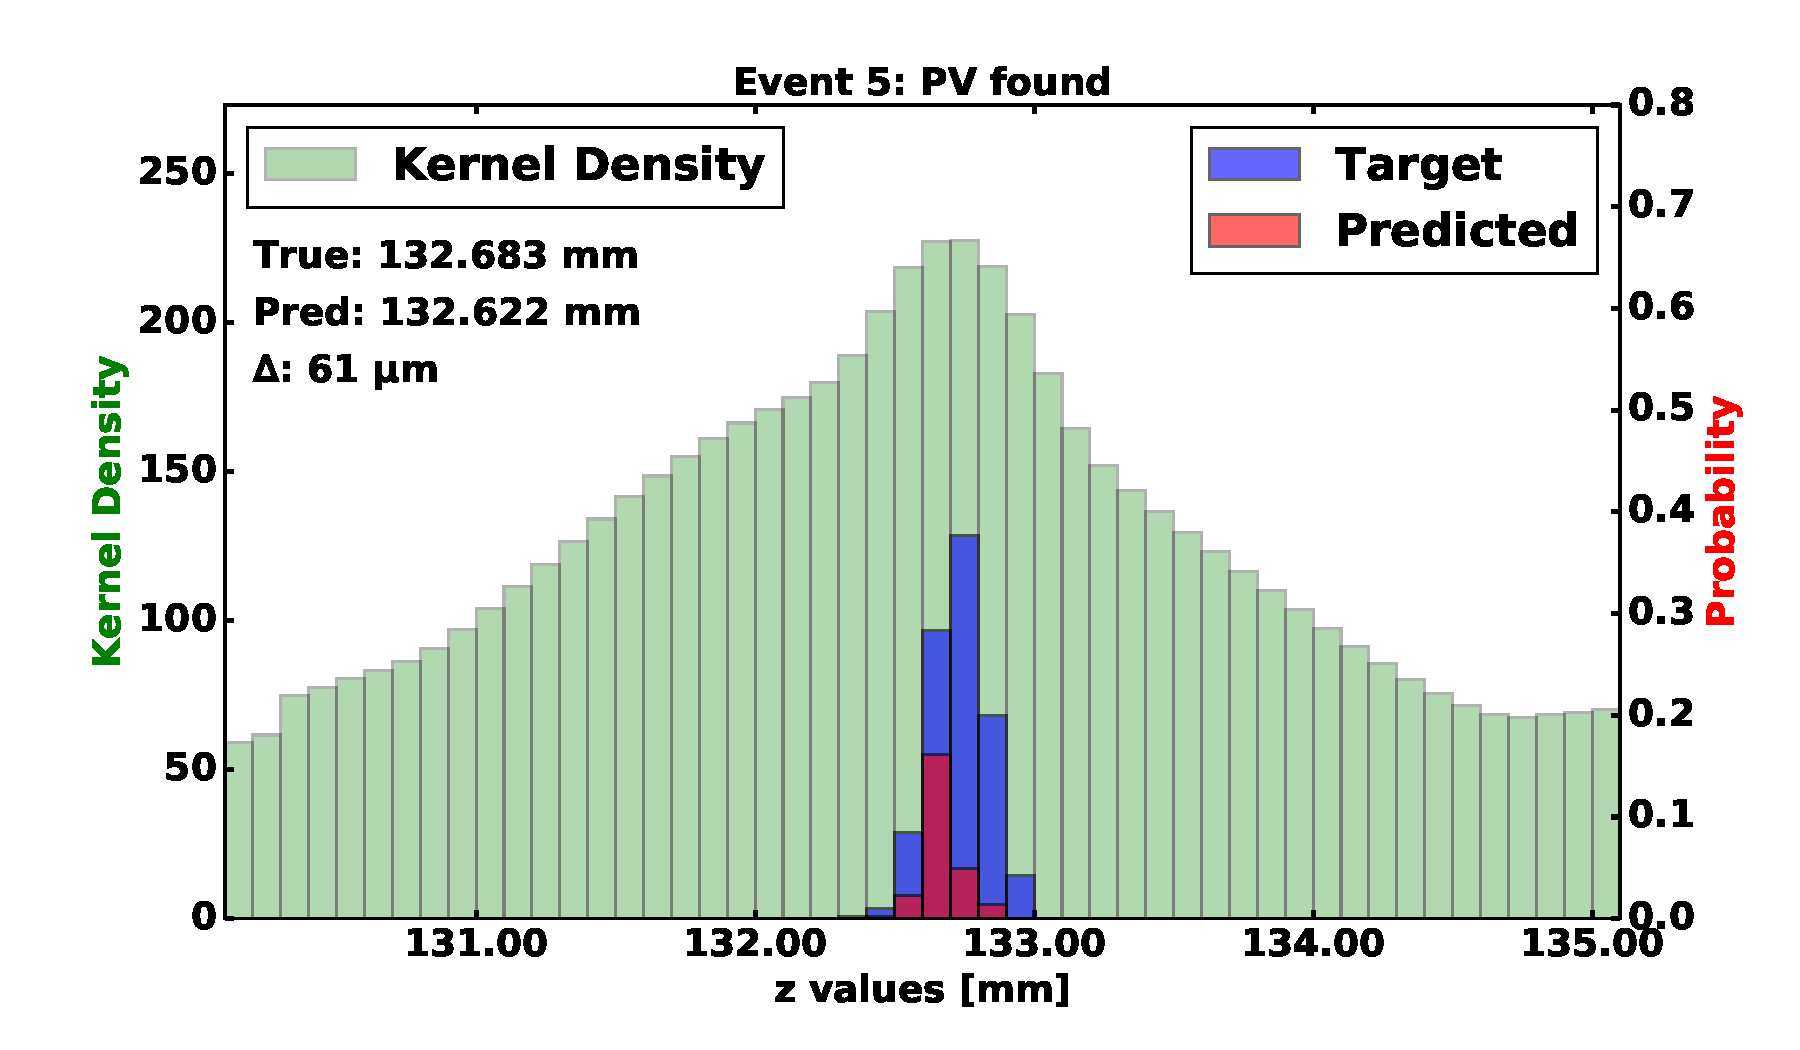
\includegraphics[width=1\textwidth, height=0.45\textwidth,trim=18 0 18 0]{images/120000_3layer_33.pdf}

        \end{center}
    \column{.5\textwidth}
        \begin{center}
           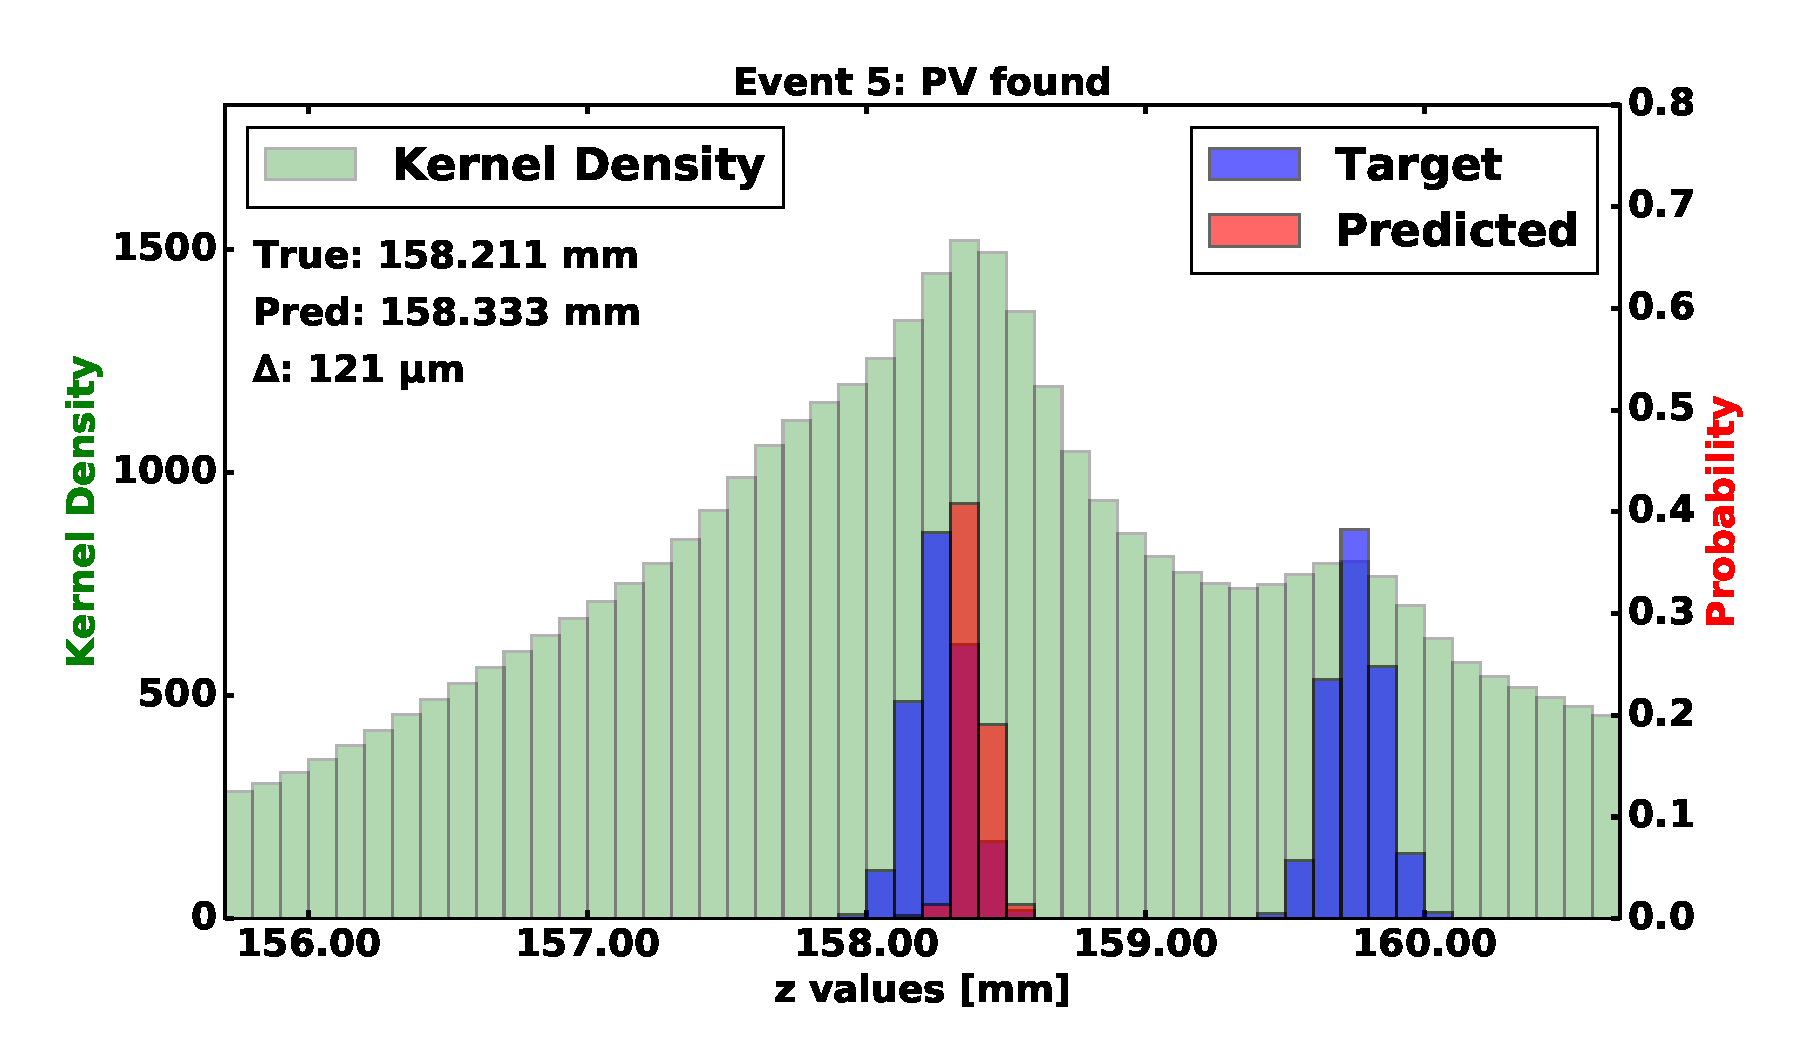
\includegraphics[width=1\textwidth, height=0.45\textwidth, trim=18 0 18 0]{images/120000_3layer_34.pdf}
    
           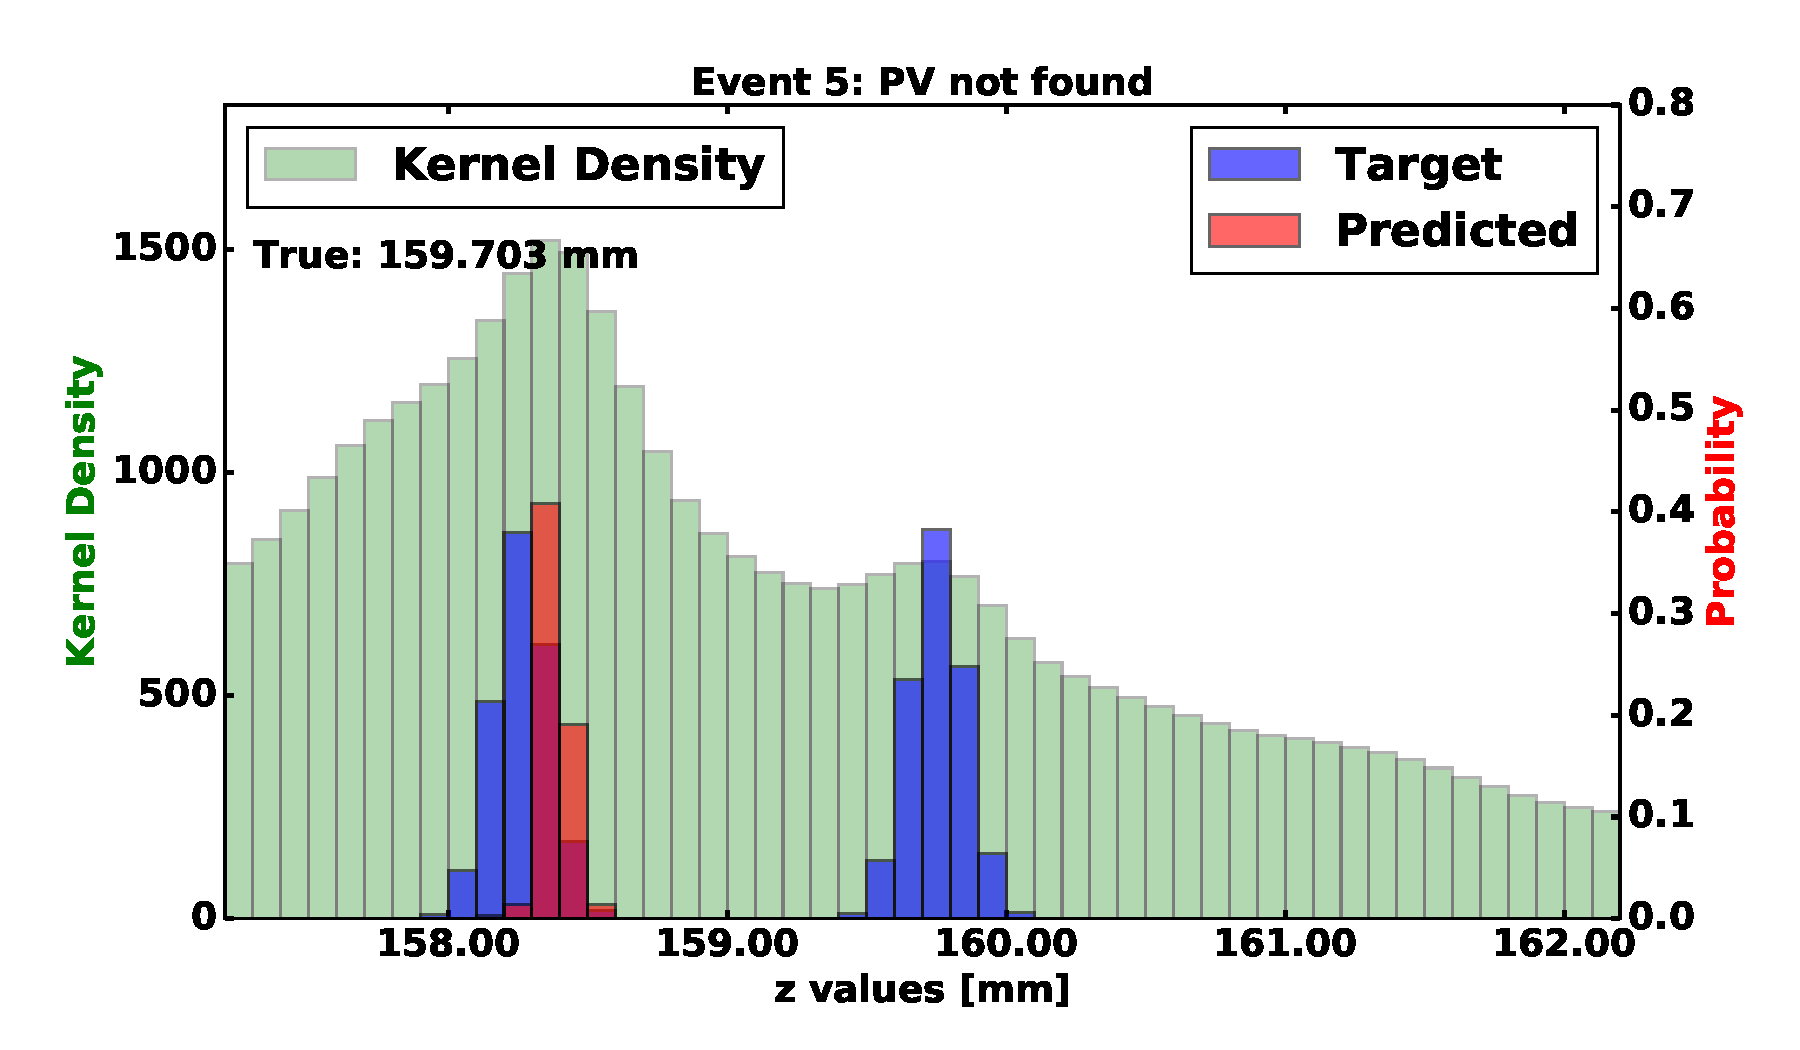
\includegraphics[width=1\textwidth, height=0.45\textwidth, trim=18 0 18 0]{images/120000_3layer_35.pdf}
       \end{center}
  \end{columns}
\end{frame}

\begin{frame}{More Predictions with Targets (3 CVN layers)}
  \begin{columns}[c]
    \column{.5\textwidth}
        \begin{center}
            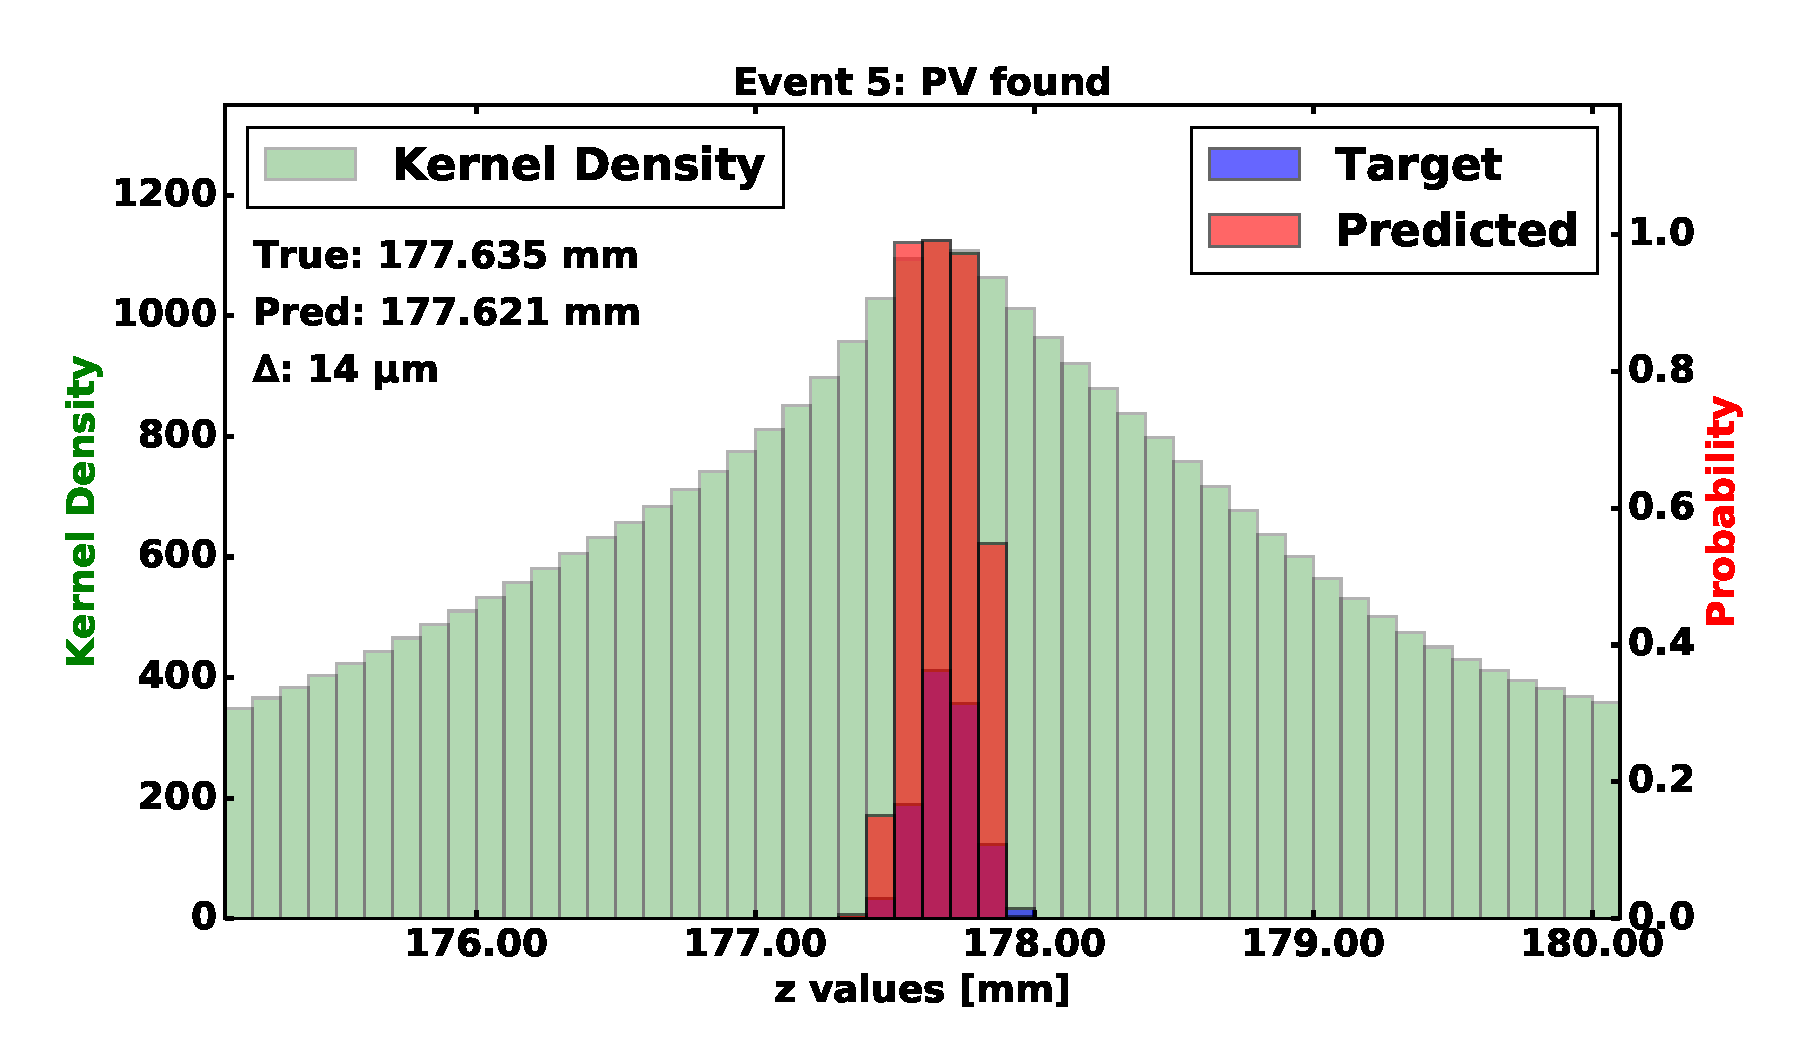
\includegraphics[width=1\textwidth,height=0.45\textwidth, trim=18 0 18 0]{images/120000_3layer_36.pdf}
    
            \includegraphics[width=1\textwidth, height=0.45\textwidth,trim=18 0 18 0]{images/120000_3layer_37.pdf}

        \end{center}
    \column{.5\textwidth}
        \begin{center}
           \includegraphics[width=1\textwidth, height=0.45\textwidth, trim=18 0 18 0]{images/120000_3layer_38.pdf}
    
           \includegraphics[width=1\textwidth, height=0.45\textwidth, trim=18 0 18 0]{images/120000_3layer_39.pdf}
       \end{center}
  \end{columns}
\end{frame}

\begin{frame}{More Predictions with Targets (3 CVN layers)}
  \begin{columns}[c]
    \column{.5\textwidth}
        \begin{center}
            \includegraphics[width=1\textwidth,height=0.45\textwidth, trim=18 0 18 0]{images/120000_3layer_40.pdf}
    
            \includegraphics[width=1\textwidth, height=0.45\textwidth,trim=18 0 18 0]{images/120000_3layer_41.pdf}

        \end{center}
    \column{.5\textwidth}
        \begin{center}
           \includegraphics[width=1\textwidth, height=0.45\textwidth, trim=18 0 18 0]{images/120000_3layer_42.pdf}
    
           \includegraphics[width=1\textwidth, height=0.45\textwidth, trim=18 0 18 0]{images/120000_3layer_43.pdf}
       \end{center}
  \end{columns}
\end{frame}

\begin{frame}{More Predictions with Targets (3 CVN layers)}
  \begin{columns}[c]
    \column{.5\textwidth}
        \begin{center}
            \includegraphics[width=1\textwidth,height=0.45\textwidth, trim=18 0 18 0]{images/120000_3layer_45.pdf}
    
            \includegraphics[width=1\textwidth, height=0.45\textwidth,trim=18 0 18 0]{images/120000_3layer_46.pdf}

        \end{center}
    \column{.5\textwidth}
        \begin{center}
           \includegraphics[width=1\textwidth, height=0.45\textwidth, trim=18 0 18 0]{images/120000_3layer_47.pdf}
    
           \includegraphics[width=1\textwidth, height=0.45\textwidth, trim=18 0 18 0]{images/120000_3layer_48.pdf}
       \end{center}
  \end{columns}
\end{frame}

\begin{frame}{More Predictions with Targets (3 CVN layers)}
  \begin{columns}[c]
    \column{.5\textwidth}
        \begin{center}
            \includegraphics[width=1\textwidth,height=0.45\textwidth, trim=18 0 18 0]{images/120000_3layer_49.pdf}
    
            \includegraphics[width=1\textwidth, height=0.45\textwidth,trim=18 0 18 0]{images/120000_3layer_50.pdf}

        \end{center}
    \column{.5\textwidth}
        \begin{center}
           \includegraphics[width=1\textwidth, height=0.45\textwidth, trim=18 0 18 0]{images/120000_3layer_51.pdf}
    
           \includegraphics[width=1\textwidth, height=0.45\textwidth, trim=18 0 18 0]{images/120000_3layer_52.pdf}
       \end{center}
  \end{columns}
\end{frame}

\begin{frame}{More Predictions with Targets (3 CVN layers)}
  \begin{columns}[c]
    \column{.5\textwidth}
        \begin{center}
            \includegraphics[width=1\textwidth,height=0.45\textwidth, trim=18 0 18 0]{images/120000_3layer_53.pdf}
    
            \includegraphics[width=1\textwidth, height=0.45\textwidth,trim=18 0 18 0]{images/120000_3layer_54.pdf}

        \end{center}
    \column{.5\textwidth}
        \begin{center}
           \includegraphics[width=1\textwidth, height=0.45\textwidth, trim=18 0 18 0]{images/120000_3layer_55.pdf}
    
           \includegraphics[width=1\textwidth, height=0.45\textwidth, trim=18 0 18 0]{images/120000_3layer_56.pdf}
       \end{center}
  \end{columns}
\end{frame}



\backupend


\end{document}
